%% (Master) Thesis template
%% Template version used: v1.4 (CADMO, ETHZ)
%%
%% Largely adapted from Adrian Nievergelt's template for the ADPS
%% (lecture notes) project.

%%%%%%%%%%%%%%%%%%%%%%%%%%%%%%%%%%%%%%%%%%%%%%%%%%%%%%%%%%%%%%%%%%%%%%%%%%%%%%%
%%%  Document settings                                                      %%%
%%%%%%%%%%%%%%%%%%%%%%%%%%%%%%%%%%%%%%%%%%%%%%%%%%%%%%%%%%%%%%%%%%%%%%%%%%%%%%%

%% We use the memoir class because it offers a many easy to use features.
\documentclass[11pt,a4paper,titlepage]{memoir}

%% LaTeX Font encoding -- DO NOT CHANGE
\usepackage[T1]{fontenc}

%% Babel provides support for languages.  'english' uses British
%% English hyphenation and text snippets like "Figure" and
%% "Theorem". Use the option 'ngerman' if your document is in German.
%% Use 'american' for American English.  Note that if you change this,
%% the next LaTeX run may show spurious errors.  Simply run it again.
%% If they persist, remove the .aux file and try again.
\usepackage[english]{babel}

%% Input encoding 'utf8'. In some cases you might need 'utf8x' for
%% extra symbols. Not all editors, especially on Windows, are UTF-8
%% capable, so you may want to use 'latin1' instead.
\usepackage[utf8]{inputenc}

%% This changes default fonts for both text and math mode to use Herman Zapfs
%% excellent Palatino font.  Do not change this.
\usepackage[sc]{mathpazo}

%% The AMS-LaTeX extensions for mathematical typesetting.  Do not
%% remove.
\usepackage{amsmath,amssymb,amsfonts,mathrsfs}

%% NTheorem is a reimplementation of the AMS Theorem package. This
%% will allow us to typeset theorems like examples, proofs and
%% similar.  Do not remove.
%% NOTE: Must be loaded AFTER amsmath, or the \qed placement will
%% break
\usepackage[amsmath,thmmarks]{ntheorem}

%% LaTeX' own graphics handling
\usepackage{graphicx}

%% This allows you to add .pdf files. It is used to add the
%% declaration of originality.
\usepackage{pdfpages}

%% Some more packages that you may want to use.  Have a look at the
%% file, and consult the package docs for each.
%% See the TeXed file for more explanations

%% [OPT] Multi-rowed cells in tabulars
\usepackage{multirow}

%% [REC] Intelligent cross reference package. This allows for nice
%% combined references that include the reference and a hint to where
%% to look for it.
\usepackage{varioref}

%% [OPT] Easily changeable quotes with \enquote{Text}
\usepackage[german=swiss]{csquotes}

%% [REC] Format dates and time depending on locale
\usepackage{datetime}

%% [OPT] Provides a \cancel{} command to stroke through mathematics.
%\usepackage{cancel}

%% [NEED] This allows for additional typesetting tools in mathmode.
%% See its excellent documentation.
\usepackage{mathtools}

%% [ADV] Conditional commands
%\usepackage{ifthen}

%% [OPT] Manual large braces or other delimiters.
%\usepackage{bigdelim, bigstrut}

%% [REC] Alternate vector arrows. Use the command \vv{} to get scaled
%% vector arrows.
\usepackage[h]{esvect}

%% [NEED] Some extensions to tabulars and array environments.
\usepackage{array}

%% [OPT] Postscript support via pstricks graphics package. Very
%% diverse applications.
%\usepackage{pstricks,pst-all}

%% [?] This seems to allow us to define some additional counters.
%\usepackage{etex}

%% [ADV] XY-Pic to typeset some matrix-style graphics
%\usepackage[all]{xy}

%% [OPT] This is needed to generate an index at the end of the
%% document.
%\usepackage{makeidx}

%% [OPT] Fancy package for source code listings.  The template text
%% needs it for some LaTeX snippets; remove/adapt the \lstset when you
%% remove the template content.
\usepackage[outputdir=.build]{minted}
\usepackage[most]{tcolorbox}
\usepackage{float}
\usepackage{afterpage}

%% [REC] Fancy character protrusion.  Must be loaded after all fonts.
\usepackage[activate]{pdfcprot}

%% [REC] Nicer tables.  Read the excellent documentation.
\usepackage{booktabs}

%% bibliography related
\usepackage[natbib,
  authordate,
  backend=biber,
  isbn=false,
  numbermonth=false]{biblatex-chicago}
\bibliography{mendeley}
%% non-utf8 characters imported by mendeley into the bibliography
\DeclareUnicodeCharacter{2010}{-}
\DeclareUnicodeCharacter{0301}{/}
%% hide language field/url in certain types
\DeclareSourcemap{
  \maps{
    \map{
      \step[fieldset=language, null]
    }
    \map{
      \pertype{article}
      \pertype{book}
      \pertype{inbook}
      \step[fieldset=url, null]
    }
  }
}
% enable linebreaks after the doi keyword
\DeclareFieldFormat{doi}{%
  \textrm{doi}\addcolon\allowbreak
  \ifhyperref
    {\href{http://dx.doi.org/#1}{\nolinkurl{#1}}}
    {\nolinkurl{#1}}}
% settings for linebreak penalties in urls/dois
\setcounter{biburllcpenalty}{100}
\setcounter{biburlucpenalty}{200}
% remove dashes in repeat authors
\makeatletter
\AtEveryBibitem{%
  \global\undef\bbx@lasthash%
  \clearfield{extrayear}}
\makeatother

%% glossary/acronyms
\usepackage[nogroupskip, toc]{glossaries}
\glsdisablehyper
\makeglossaries

%% greek letters in text mode
\usepackage[euler]{textgreek}

%% checkmark and other symbols
%\usepackage{pifont}

%% rotate cells in tables
\usepackage[figuresright]{rotating}

%% for degree symbols and other unit stuffs
\usepackage[binary-units=true]{siunitx}

%% inline lists
\usepackage[inline]{enumitem}

%% stoichiometric formulae and chemical equations
\usepackage[version=4]{mhchem}

%% capability for multiple footnotes & footnotes in section headings
\usepackage[multiple, stable]{footmisc}

%% for indicator function 1
\usepackage{dsfont}

%% Our layout configuration.  DO NOT CHANGE.
%% Memoir layout setup

%% NOTE: You are strongly advised not to change any of them unless you
%% know what you are doing.  These settings strongly interact in the
%% final look of the document.

%% Title page: redefine maketitle macro
\newlength{\logounitlength}
\setlength{\logounitlength}{0.08mm}

\def\thesistype#1{\def\thesistypestring{#1}}
\def\thesistypestring{}
\def\thesisperiod#1{\def\thesisperiodstring{#1}}
\def\thesisperiodstring{}
\def\thesistitle#1{\def\thesistitlestring{#1}}
\def\thesistitlestring{}
\def\thesisauthor#1{\def\thesisauthorstring{#1}}
\def\thesisauthorstring{}
\def\submissiondate#1{\def\submissiondatestring{#1}}
\def\submissiondatestring{}
\def\alternatereader#1{\def\alternatereaderstring{#1}}
\def\alternatereaderstring{}
\def\mainreader#1{\def\mainreaderstring{#1}}
\def\mainreaderstring{}

\newcommand{\ETHlogo}{
  \parbox{100mm}{
    \vbox{
      \kern2pt\setlength{\unitlength}{\logounitlength}
      \begin{picture}(330,110)(0,-5)
        \thicklines
        \multiput(0,0)(2,0){16}{\line(1,4){25}}
        \multiput(1,0)(0.5,2){12}{\line(1,0){84}}
        \multiput(42,40.4)(0.5,2){11}{\line(1,0){53}}
        \multiput(19.5,78.8)(0.5,2){12}{\line(1,0){210}}
        \multiput(116,0)(2,0){16}{\line(1,4){24}}
        \multiput(180,0)(2,0){16}{\line(1,4){25}}
        \multiput(237,0)(2,0){16}{\line(1,4){25}}
        \multiput(220,39)(0.5,2){12}{\line(1,0){30}}
        \put(262.5,100){\line(1,0){30}}
      \end{picture}
      \hfill\break\sffamily\bfseries Swiss Federal Institute of Technology 
      Zurich
    }
  }
}

\newcommand{\SfSlogo}{
  \parbox{40mm}{
    \hfill\kern2pt
    \setlength{\unitlength}{\logounitlength}\begin{picture}(330,110)(0,-5)
    \end{picture}\\
    \sffamily\bfseries
    \null\hfill Seminar for\kern3mm\break
    \null\hfill \phantom{g}Statistics\kern3mm%
  }
}

\makeatletter
\def\maketitle{
  \begingroup
  \hspace*{-3pt}\raise 20pt\hbox{\ETHlogo}\hfill
    \raise 19pt\hbox{\SfSlogo}\hspace*{-10pt}
  \linebreak
  \vspace{1pt}
  {\sffamily\bfseries\noindent{\\Departement of Mathematics}}
  \par\vspace*{5pt}
  \rule{\linewidth}{.3pt}\\[1pt]
  \vspace*{-15pt}
  \begin{center}
    \Large \thesistypestring
    \hfill
    \Large \thesisperiodstring\\[2pt] 
  \end{center}
  \rule{\linewidth}{.3pt}
  \medskip
  \vspace{70pt}
  \begin{center}
    \bfseries
    \Large \thesisauthorstring\\
    \vspace{2ex plus 1ex minus 1.5ex}
    \LARGE \thesistitlestring
  \end{center}
  \vspace{\stretch{2}}
  \vspace{\stretch{3}}

  \begin{center} \large
    \rule{.5\linewidth}{.3pt} \\[8pt]
    \begin{tabular}{ll}
      Submission Date: & \submissiondatestring
    \end{tabular}
    \\[5pt] \rule{.5\linewidth}{.3pt}
    
    \vspace{2ex plus 25ex minus 1.5ex}
    
    \begin{tabular}{ll}
      Co-Adviser: & \alternatereaderstring \\
      Adviser:    & \mainreaderstring
    \end{tabular}
  \end{center}
  \vspace*{-20pt}

  \endgroup
}
\makeatother

%% Turn extra space before chapter headings off.
\setlength{\beforechapskip}{0pt}

\nonzeroparskip
\parindent=0pt
\defaultlists

%% Chapter style redefinition
\makeatletter

\if@twoside
  \pagestyle{Ruled}
  \copypagestyle{chapter}{Ruled}
\else
  \pagestyle{ruled}
  \copypagestyle{chapter}{ruled}
\fi
\makeoddhead{chapter}{}{}{}
\makeevenhead{chapter}{}{}{}
\makeheadrule{chapter}{\textwidth}{0pt}
\copypagestyle{abstract}{empty}

\makechapterstyle{bianchimod}{%
  \chapterstyle{default}
  \renewcommand*{\chapnamefont}{\normalfont\Large\sffamily}
  \renewcommand*{\chapnumfont}{\normalfont\Large\sffamily}
  \renewcommand*{\printchaptername}{%
    \chapnamefont\centering\@chapapp}
  \renewcommand*{\printchapternum}{\chapnumfont {\thechapter}}
  \renewcommand*{\chaptitlefont}{\normalfont\huge\sffamily}
  \renewcommand*{\printchaptertitle}[1]{%
    \hrule\vskip\onelineskip \centering \chaptitlefont\textbf{\vphantom{gyM}##1}\par}
  \renewcommand*{\afterchaptertitle}{\vskip\onelineskip \hrule\vskip
    \afterchapskip}
  \renewcommand*{\printchapternonum}{%
    \vphantom{\chapnumfont {9}}\afterchapternum}}

%% Use the newly defined style
\chapterstyle{bianchimod}

\setsecheadstyle{\Large\bfseries\sffamily}
\setsubsecheadstyle{\large\bfseries\sffamily}
\setsubsubsecheadstyle{\bfseries\sffamily}
\setparaheadstyle{\normalsize\bfseries\sffamily}
\setsubparaheadstyle{\normalsize\itshape\sffamily}
\setsubparaindent{0pt}

%% Set captions to a more separated style for clearness
\captionnamefont{\sffamily\bfseries\footnotesize}
\captiontitlefont{\sffamily\footnotesize}
\setlength{\intextsep}{16pt}
\setlength{\belowcaptionskip}{1pt}

%% Set section and TOC numbering depth to subsection
\setsecnumdepth{subsection}
\settocdepth{subsection}

\checkandfixthelayout

\setlength{\droptitle}{-48pt}

\makeatother

%% This defines how theorems should look. Best leave as is.
\theoremstyle{plain}
\setlength\theorempostskipamount{0pt}

%% customized appearance for some characters
\renewcommand{\tilde}{\hbox{\raise.17ex\hbox{$\scriptstyle\mathtt{\sim}$}}}

%% fixed width columns in table with text justification
\newcolumntype{L}[1]{>{\raggedright\let\newline\\\arraybackslash\hspace{0pt}}m{#1}}
\newcolumntype{C}[1]{>{\centering\let\newline\\\arraybackslash\hspace{0pt}}m{#1}}
\newcolumntype{R}[1]{>{\raggedleft\let\newline\\\arraybackslash\hspace{0pt}}m{#1}}


%% Theorem environments.  You will have to adapt this for a German
%% thesis.
%% Theorem-like environments

%% This can be changed according to language. You can comment out the ones you
%% don't need.

\numberwithin{equation}{chapter}

%% English variants
\newtheorem{theorem}{Theorem}[chapter]
\newtheorem{example}[theorem]{Example}
\newtheorem{remark}[theorem]{Remark}
\newtheorem{corollary}[theorem]{Corollary}
\newtheorem{definition}[theorem]{Definition}
\newtheorem{lemma}[theorem]{Lemma}
\newtheorem{proposition}[theorem]{Proposition}

%% Proof environment with a small square as a "qed" symbol
\theoremstyle{nonumberplain}
\theorembodyfont{\normalfont}
\theoremsymbol{\ensuremath{\square}}
\newtheorem{proof}{Proof}
%\newtheorem{beweis}{Beweis}


%% Helpful macros.
%% Custom commands
%% ===============

%% enable glossary style to be reversed in select instances
\newcommand*\glsrev[2][]{%
  \ifglsused{#2}{%
    %% subsequent use
    \glsdisp[#1]{#2}{\glsentryshort{#2}}%
  }{%
    %% first use
    \glsdisp[#1]{#2}{\glsentryshort{#2}\space(\glsentrylong{#2})}%
  }%
}
\newcommand*\Glsrev[2][]{%
  \ifglsused{#2}{%
    %% subsequent use
    \glsdisp[#1]{#2}{\Glsentryshort{#2}}%
  }{%
    %% first use
    \glsdisp[#1]{#2}{\Glsentryshort{#2}\space(\glsentrylong{#2})}%
  }%
}
\newcommand*\glsrevpl[2][]{%
  \ifglsused{#2}{%
    %% subsequent use
    \glsdisp[#1]{#2}{\glsentryshortpl{#2}}%
  }{%
    %% first use
    \glsdisp[#1]{#2}{\glsentryshortpl{#2}\space(\glsentrylongpl{#2})}%
  }%
}
\newcommand*\Glsrevpl[2][]{%
  \ifglsused{#2}{%
    %% subsequent use
    \glsdisp[#1]{#2}{\Glsentryshortpl{#2}}%
  }{%
    %% first use
    \glsdisp[#1]{#2}{\Glsentryshortpl{#2}\space(\glsentrylongpl{#2})}%
  }%
}

%% Special characters for number sets, e.g. real or complex numbers.
\newcommand{\C}{\mathbb{C}}
\newcommand{\K}{\mathbb{K}}
\newcommand{\Nat}{\mathbb{N}}
\newcommand{\Q}{\mathbb{Q}}
\newcommand{\R}{\mathbb{R}}
\newcommand{\Z}{\mathbb{Z}}
\newcommand{\X}{\mathbb{X}}

%% Fixed/scaling delimiter examples (see mathtools documentation)
\DeclarePairedDelimiter\abs{\lvert}{\rvert}
\DeclarePairedDelimiter\norm{\lVert}{\rVert}

%% Use the alternative epsilon per default and define the old one as \oldepsilon
\let\oldepsilon\epsilon
\renewcommand{\epsilon}{\ensuremath\varepsilon}

%% Also set the alternate phi as default.
\let\oldphi\phi
\renewcommand{\phi}{\ensuremath{\varphi}}

\newcommand\given[1][]{\:#1\vert\:}
\let\existstemp\exists
\let\foralltemp\forall
\renewcommand{\exists}{\ensuremath\enskip\existstemp\:}
\renewcommand{\forall}{\ensuremath\enskip\foralltemp\:}

%% excerpts from SfS texab.sty
%% ===========================
%% R program
\newcommand*{\Rp}{\textsf{R}$\;$}
%% the epsfCfile function used in an example
\makeatletter
\newcommand{\@epsFFile}[2]{\includegraphics[#1]{#2}}
\newcommand{\epsFracFile}[2]{\@epsFFile{width=#1\textwidth}{#2}}%
\newcommand{\epsFracFileRot}[3][-90]{\@epsFFile{angle=#1,width=#2\textwidth}{#3}}
\newcommand{\epsfCfile}[2]{\centerline{\epsFracFile{#1}{#2}}}%
\newcommand{\epsfCfileRot}[3][-90]{\centerline{\epsFracFileRot[#1]{#2}{#3}}}%
\makeatother

\DeclareMathOperator{\logit}{logit}
\DeclareMathOperator{\med}{med}
\DeclareMathOperator{\median}{median}
\DeclareMathOperator{\Med}{Med}
\DeclareMathOperator{\Erw}{\mathbf{E}}%-- see also \E (below)
\DeclareMathOperator{\var}{var}
\DeclareMathOperator{\Var}{Var}
\DeclareMathOperator{\Cov}{Cov}
\DeclareMathOperator{\cov}{cov}
\DeclareMathOperator{\Cor}{Corr}
\DeclareMathOperator{\cor}{corr}
\DeclareMathOperator{\se}{se}
\DeclareMathOperator{\sd}{sd}
\DeclareMathOperator{\sign}{sign}
\DeclareMathOperator{\trace}{tr}
\DeclareMathOperator{\const}{const}
\DeclareMathOperator{\diag}{diag}
%% Nachteil von diesen (wegen \limits !?): \argmax_\beta setzt \beta
%% *unterhalb*, auch inline, was  \max_\beta nicht tut
%% \newcommand{\argmin}{\mathop{\arg \min}\limits}
%% \newcommand{\argmax}{\mathop{\arg \max}\limits}
%% \newcommand{\ave}{\mathop{ave}\limits}
%% This is following http://en.wikipedia.org/wiki/Arg_max 's recommendation:
\DeclareMathOperator*{\ave}{ave}
\DeclareMathOperator*{\argmin}{arg\, min}
\DeclareMathOperator*{\argmax}{arg\, max}
%
\DeclareMathOperator{\IF}{IF}
\DeclareMathOperator{\und}{ und }
\DeclareMathOperator{\oder}{ oder }
%\def\mit{\mathrm{ mit }}  %-- causes some problems with \mbox or \boldmath !!!
\DeclareMathOperator{\for}{ for }
\DeclareMathOperator{\where}{ where }
\DeclareMathOperator{\with}{ with }
%%-------  NB.  << NEVER >> REdefine  \or !!! ----
%% Not ``\and'': this is used in \author

% - Math. Operatoren
\newcommand{\op}[1]{\mathop{#1}}%was\newcommand{\op}[1]{\kern-.2em #1\kern-.2em}
% \newcommand{\oneover}[1]{{1\over#1}\,\,}
\newcommand{\oneover}[1]{{\textstyle 1\over#1}}
\newcommand{\inv}{^{-1}}
\newcommand{\sups}[1]{^{(#1)}}
%%-- shorter, for convergence ...==== unnecessary ===
%%-- There is already \to  (in standard TeX & LaTeX !) :
\newcommand{\go}{\rightarrow%
        \typeout{use standard \TeX \verb|\to| instead of \verb|\go|}}
%% convergence in Probability, Distribution: \tendsto{P}, \tendsto{D} :
\newcommand{\tendsto}[1]{\buildrel {#1} \over \longrightarrow}
\newcommand{\wt}{\widetilde}
\newcommand{\wh}[1]{\if \sigma{#1}\widehat{\sigma}\else
{}\kern0.1em\widehat{\kern-0.1em#1}{}\fi}
\newcommand{\wb}[1]{{}\if Y#1\overline{Y}\else
\kern0.2em\overline{\kern-0.2em#1}\fi}
\newcommand{\Ssum}{\sum\nolimits}
\newcommand{\Sn}{\Ssum_{i=1}^n}
\newcommand{\Seq}[4]{#1_{#2},\,#1_{#3},\ldots,#1_{#4}}% siehe auch \Nl , \No (unten)
\newcommand{\Half}{{\textstyle 1\over2}}% siehe auch \half (unten)
\newcommand{\ul}[1]{\textbf{#1}}

\newcommand{\Hmu}{\widehat{\mu}}
\newcommand{\Halpha}{\widehat{\alpha}}
\newcommand{\Hbeta}{\widehat{\beta}}
%
\newcommand{\iid}{\mbox{ i.i.d. }}
\newcommand{\fs}{\mbox{f.s.}}
\newcommand{\Loglik}{\ell\kern-1pt\ell}

%%%------------ script und andere Spezialschriften ----------------------


\DeclareMathOperator{\N}{\mathcal{N}}% Normalverteilung
\renewcommand{\P}{\mathcal{P}}%--- RE-defining the standard \P (Paragraph)!!--
%%%
\DeclareMathOperator{\M}{\mathcal{M}}% Multinom ?
\DeclareMathOperator{\B}{\mathcal{B}}% Binom
\DeclareMathOperator{\Bern}{\mathcal{B}ernoulli}
\DeclareMathOperator{\E}{\mathcal{E}}%-- see also \Erw (above)
\DeclareMathOperator{\F}{\mathcal{F}}
\DeclareMathOperator{\Wish}{\mathcal{W}}
\newcommand{\phibf}{\boldsymbol{\phi}}%{\phi\hskip-5.4pt\phi} % bold \phi


%% Make document internal hyperlinks wherever possible. (TOC, references)
%% This MUST be loaded after varioref, which is loaded in 'extrapackages'
%% above.  We just load it last to be safe.
\usepackage{hyperref}
\definecolor{Blue}{rgb}{0,0,0.8}
\definecolor{Red}{rgb}{0.7,0,0}
\hypersetup{
  %hyperindex,
  colorlinks={true},
  %pagebackref,
  linktocpage,
  plainpages={false},
  linkcolor={Blue},
  citecolor={Blue},
  urlcolor={Red},
  pdfstartview={Fit},
  pdfview={XYZ null null null}
}


%% Set the paths where all figures are taken from:
\graphicspath{{figures/}}
%% level on which equation numbering is done
\numberwithin{equation}{chapter}
%% import knitr related stuff
\usepackage[]{graphicx}\usepackage[]{color}
%% maxwidth is the original width if it is less than linewidth
%% otherwise use linewidth (to make sure the graphics do not exceed the margin)
\makeatletter
\def\maxwidth{ %
  \ifdim\Gin@nat@width>\linewidth
    \linewidth
  \else
    \Gin@nat@width
  \fi
}
\makeatother

\definecolor{fgcolor}{rgb}{0.345, 0.345, 0.345}
\newcommand{\hlnum}[1]{\textcolor[rgb]{0.686,0.059,0.569}{#1}}%
\newcommand{\hlstr}[1]{\textcolor[rgb]{0.192,0.494,0.8}{#1}}%
\newcommand{\hlcom}[1]{\textcolor[rgb]{0.678,0.584,0.686}{\textit{#1}}}%
\newcommand{\hlopt}[1]{\textcolor[rgb]{0,0,0}{#1}}%
\newcommand{\hlstd}[1]{\textcolor[rgb]{0.345,0.345,0.345}{#1}}%
\newcommand{\hlkwa}[1]{\textcolor[rgb]{0.161,0.373,0.58}{\textbf{#1}}}%
\newcommand{\hlkwb}[1]{\textcolor[rgb]{0.69,0.353,0.396}{#1}}%
\newcommand{\hlkwc}[1]{\textcolor[rgb]{0.333,0.667,0.333}{#1}}%
\newcommand{\hlkwd}[1]{\textcolor[rgb]{0.737,0.353,0.396}{\textbf{#1}}}%

\usepackage{framed}
\makeatletter
\newenvironment{kframe}{%
 \def\at@end@of@kframe{}%
 \ifinner\ifhmode%
  \def\at@end@of@kframe{\end{minipage}}%
  \begin{minipage}{\columnwidth}%
 \fi\fi%
 \def\FrameCommand##1{\hskip\@totalleftmargin \hskip-\fboxsep
 \colorbox{shadecolor}{##1}\hskip-\fboxsep
     % There is no \\@totalrightmargin, so:
     \hskip-\linewidth \hskip-\@totalleftmargin \hskip\columnwidth}%
 \MakeFramed {\advance\hsize-\width
   \@totalleftmargin\z@ \linewidth\hsize
   \@setminipage}}%
 {\par\unskip\endMakeFramed%
 \at@end@of@kframe}
\makeatother

\definecolor{shadecolor}{rgb}{.97, .97, .97}
\definecolor{messagecolor}{rgb}{0, 0, 0}
\definecolor{warningcolor}{rgb}{1, 0, 1}
\definecolor{errorcolor}{rgb}{1, 0, 0}
\newenvironment{knitrout}{}{} % an empty environment to be redefined in TeX

\usepackage{alltt}



%% glossary definitions
%% cellular biochemistry
% t3ss
\newacronym{t3ss}{T3SS}{type III secretion system}
\newacronym{ipa}{Ipa}{\textit{Shigella} invasion protein}
\newacronym{sop}{Sop}{\textit{Salmonella} outer protein}
% general
\newacronym{gtp}{GTP}{guanosine triphosphate}
\newacronym{gdp}{GDP}{guanosine diphosphate}
\newacronym{gef}{GEF}{guanine nucleotide exchange factor}
\newacronym{gap}{GAP}{GTPase activating protein}
%% cell biology
\newacronym{erad}{ERAD}{endoplasmic-reticulum-associated protein degradation}
\newacronym{er}{ER}{endoplasmic reticulum}

\newacronym{tir}{Tir}{translocated intimin receptor}
\newacronym{rac-1}{Rac1}{Ras-related C3 botulinum toxin substrate 1}
\newacronym{arp23}{Arp2/3}{actin-related-protein 2 and 3}
\newacronym{sip}{Sip}{\textit{Salmonella} invasion protein}
\newacronym{cdc-42}{Cdc42}{cell division control protein 42 homolog}
\newacronym{spt-p}{SptP}{secreted effector protein}
\newacronym{t4ss}{T4SS}{type IV secretion system}
\newacronym{vegf}{VEGF}{vascular endothelial growth factor}
\newacronym{icam-1}{ICAM-1}{interleukin-8}
\newacronym{il-8}{IL-8}{intercellular adhesion molecule 1}
\newacronym{lps}{LPS}{lipopolysaccharide}
\newacronym{tlr}{TLR}{toll-like receptor}
\newacronym{prpc}{PrPC}{cellular prion protein}
\newacronym{hsp}{HSP}{heat shock protein}
\newacronym{tir-1}{TIR}{toll-interleukin-1 receptor}
\newacronym{mhc}{MHC}{major histocompatibility complex}
\newacronym{ergic}{ERGIC}{ER-Golgi intermediate compartment}
\newacronym{cop-2}{COPII}{coat protein complex II, involved in anterograde \gls{er}--Golgi transport}
\newacronym{atr}{ATR}{acid tolerance response}
\newacronym{tap}{TAP}{tapasin}
\newacronym{mapk}{MAPK}{mitogen-activated protein kinase}
\newacronym{m-cells}{M cells}{microfold cells}
\newacronym{pi45p2}{PI(4,5)P\textsubscript{2}}{phosphatidylinositol 4,5-bisphosphate}
\newacronym{pi3p}{PI(3)P}{phosphatidylinositol 3-phosphate}
\newacronym{pi4p}{PI(4)P}{phosphatidylinositol 4-phosphate}
\newacronym{pi5p}{PI(5)P}{phosphatidylinositol 5-phosphate}
\newacronym{i13456p5}{I(1,3,4,5,6)P\textsubscript{5}}{inositol 1,3,4,5,6-pentakisphosphate}
\newacronym{i1456p4}{I(1,4,5,6)P\textsubscript{4}}{inositol 1,4,5,6-tetrakisphosphate}
\newacronym{abm}{ABM}{actin based motility}
\newacronym{lcv}{LCV}{\textit{Legionella}-containing vacuole}
\newacronym{npf}{NPF}{nucleation promoting factor}
\newacronym{sp41}{SP41}{\textit{Brucella} surface protein}
\newacronym{cbg}{C\textbeta G}{\textit{Brucella} cyclic \textbeta-1,2-glucan}
\newacronym{bacv}{BaCV}{\textit{Bartonella}-containing vacuole}
\newacronym{brcv}{BrCV}{\textit{Brucella}-containing vacuole}
\newacronym{fcv}{FCV}{\textit{Francisella}-containing vacuole}
\newacronym{scv}{SCV}{\textit{Salmonella}-con\-tain\-ing vacuole}
\newacronym{spi}{SPI}{\textit{Salmonella} pathogenicity island}
\newacronym{sif}{SIF}{\textit{Salmonella}-induced filaments}
\newacronym{rho-g}{RhoG}{Ras homology growth-related}
\newacronym{ics}{Ics}{\textit{Shigella} intracellular spread protein}
\newacronym{n-wasp}{N-WASP}{neural Wiskott-Aldrich syndrome protein}
\newacronym{wasp}{WASP}{Wiskott-Aldrich syndrome protein}
\newacronym{ilk}{ILK}{integrin linked kinase}
\newacronym{car}{CAR}{coxsackievirus and adenovirus receptor}
\newacronym{nf-kb}{NF-\textkappa B}{nuclear factor \textkappa-light-chain-enhancer of activated B cells}
\newacronym[longplural={nuclear pore complexes}]{npc}{NPC}{nuclear pore complex}
\newacronym{moi}{MOI}{multiplicity of infection}
\newacronym{nls}{NLS}{nuclear localization signal}
\newacronym{ptp}{pTP}{precursor terminal protein}
\newacronym{dbp}{DBP}{DNA-binding protein}
\newacronym{vldlr}{VLDLR}{very low-density lipoprotein receptor}
\newacronym{cdhr3}{CDHR3}{cadherin-related family member 3}
\newacronym{mv}{MV}{mature virion}
\newacronym{ev}{EV}{extracellular virion}
\newacronym{ccp}{CCP}{clathrin-coated pit}
\newacronym{ccv}{CCV}{clathrin-coated vesicles}
\newacronym{mrna}{mRNA}{messenger RNA}
\newacronym{sirna}{siRNA}{short interfering RNA}
\newacronym{mirna}{miRNA}{microRNA}
\newacronym{pri-mirna}{pri-\gls{mirna}}{primary \gls{mirna}}
\newacronym{pre-mirna}{pre-\gls{mirna}}{precursor \gls{mirna}}
\newacronym{dgcr8}{DGCR8}{DiGeorge syndrome critical region gene 8}
\newacronym{trbp}{TRBP}{TRA RNA-binding protein}
\newacronym{pact}{PACT}{protein activator of protein kinase PKR}
\newacronym{risc}{RISC}{RNA-induced silencing complex}
\newacronym{ago}{Ago}{Argonaute}
\newacronym{paz}{PAZ}{PIWI-Argonaute-Zwille domain}
\newacronym{mid}{MID}{Argonaute middle domain}
\newacronym{piwi}{PIWI}{P-element-induced whimpy testes domain}
\newacronym{rits}{RITS}{RNA-induced transcriptional silencing complex}
\newacronym{rdrc}{RDRC}{RNA-dependent RNA polymerase complex}
\newacronym{pkr}{PKR}{RNA-dependent protein kinase pathway}
\newacronym{ote}{OTE}{off-target effects}
\newacronym{hts}{HTS}{high throughput screening}
\newacronym{lof}{LOF}{loss-of-function}
\newacronym{gfp}{GFP}{green fluorescent protein}
\newacronym{shrna}{shRNA}{short hairpin RNA}
\newacronym{atp}{ATP}{adenosine triphosphate}
\newacronym{llo}{LLO}{listeriolysin O}
\newacronym{gilt}{GILT}{\textgamma-interferon-inducible lysosomal thiol reductase}
\newacronym{ehec}{EHEC}{enterohemorrhagic \textit{E. coli}}
\newacronym{epec}{EPEC}{enteropathogenic \textit{E. coli}}
\newacronym{mtor}{mTOR}{mechanistic target of rapamycin}
\newacronym{ros}{ROS}{reactive oxygen species}
\newacronym{eis}{Eis}{enhanced intracellular survival protein}
\newacronym{camp}{cAMP}{cyclic adenosine monophosphate}
\newacronym{taa}{TAA}{trimeric autotransporter adhesin}
\newacronym{ecm}{ECM}{extracellular matrix}
\newacronym{kif11}{KIF11}{kinesin family member 11}
\newacronym{ppib}{PPIB}{Peptidyl-prolyl cis-trans isomerase B}
\newacronym{gapdh}{GAPDH}{glyceraldehyde-3-phosphate dehydrogenase}
\newacronym{lmna}{LMNA}{lamin A/C}

%% diseases
\newacronym{aids}{AIDS}{acquired immune deficiency syndrome}
\newacronym{csd}{CSD}{Cat Scratch Disease}
\newacronym{hiv}{HIV}{human immunodeficiency virus}
\newacronym{sars}{SARS}{severe acute respiratory syndrome}
\newacronym{amr}{AMR}{antimicrobial resistance}
\newacronym{hdt}{HDT}{host directed therapeutics}
\newacronym{cap}{CAP}{community-acquired pneumonia}
\newacronym{aav}{AAV}{adeno-associated virus}

%% misc
\newacronym{who}{WHO}{World Health Organization}
\newacronym{icu}{ICU}{intensive care unit}
\newacronym{rtd}{RTD}{research, technology and development}
\newacronym{dmem}{DMEM}{Dulbecco Modified Eagle Medium}
\newacronym{fbs}{FBS}{fetal bovine serum}
\newacronym{pfa}{PFA}{paraformaldehyde}
\newacronym{hpc}{HPC}{high performance computing}
\newacronym{hcs}{HCS}{high content screening}
\newacronym{api}{API}{application programming interface}
\newacronym{as}{AS}{application server}
\newacronym{dss}{DSS}{data store server}
\newacronym{svm}{SVM}{support vector machine}
\newacronym{dtis}{DTIS}{decision tree infection scoring}


%%%%%%%%%%%%%%%%%%%%%%%%%%%%%%%%%%%%%%%%%%%%%%%%%%%%%%%%%%%%%%%%%%%%%%%%%%%%%%%
%%%  Document body                                                          %%%
%%%%%%%%%%%%%%%%%%%%%%%%%%%%%%%%%%%%%%%%%%%%%%%%%%%%%%%%%%%%%%%%%%%%%%%%%%%%%%%

\begin{document}

\frontmatter

%%%%%%%%%%%%%%%%%%%%%%%%%%%%%%%%%%%%%%%%%%%%%%%%%%%%%%%%%%%%%%%%%%%%%%%%%%%%%%%
%%%  Title page                                                             %%%
%%%%%%%%%%%%%%%%%%%%%%%%%%%%%%%%%%%%%%%%%%%%%%%%%%%%%%%%%%%%%%%%%%%%%%%%%%%%%%%

\thesistype{Master Thesis}
\thesisperiod{Spring 2015}
\thesisauthor{Nicolas Bennett}
\thesistitle{
  The title of my thesis\\
  which should be split on\\
  several lines if it is too long
}
\submissiondate{August 25th 2015}
\mainreader{Prof.\ Dr.\ Peter Bühlmann}
\alternatereader{Anna Drewek}

\begin{titlingpage}
  \vspace*{-2cm}
  \calccentering{\unitlength}
  \begin{adjustwidth*}{\unitlength-1cm}{-\unitlength-1cm}
    \maketitle
  \end{adjustwidth*}
\end{titlingpage}

%%%%%%%%%%%%%%%%%%%%%%%%%%%%%%%%%%%%%%%%%%%%%%%%%%%%%%%%%%%%%%%%%%%%%%%%%%%%%%%
%%%  Front matter                                                           %%%
%%%%%%%%%%%%%%%%%%%%%%%%%%%%%%%%%%%%%%%%%%%%%%%%%%%%%%%%%%%%%%%%%%%%%%%%%%%%%%%

%% Dedication (optional)
%\markright{}
\vspace*{\stretch{1}}
[B]ecause we tend to reward others when they do well and punish them when they do badly, and because there is regression to the mean, it is part of the human condition that we are statistically punished for rewarding others and rewarded for punishing them --- \cite{Kahneman2012}.
\vspace*{\stretch{2}}

%% Preface (optional)
\cleartorecto
\addcontentsline{toc}{chapter}{Preface}
\chapter{Preface}

This thesis is submitted in partial fulfillment of the requirements for a Master's Degree in Interdisciplinary Sciences with a Major in Applied Mathematics and Computational Biology at the Swiss Federal Institute of Technology (Eidgenössische Technische Hochschule, ETH) Z\"urich. It contains work performed from April to August 2015 under the supervision of Dr.\ Anna Drewek and Prof.\ Dr.\ Peter B\"uhlmann.

All investigated data originates from the large-scale \acrfull{rnai} screening experiment \href{http://www.infectx.ch}{InfectX} (2010--2014) and the present work adds to its follow-up venture \href{http://www.targetinfectx.ch}{TargetInfectX} (ongoing). Both \acrfull{rtd} projects are funded by \href{http://www.systemsx.ch}{SystemsX}, the Swiss Initiative in Systems Biology, and set out to comprehensively study the human infectome for a set of common bacterial and viral pathogens. While InfectX was more focused on developing unified wet-lab procedures yielding comparable results over a broad range of pathogens and establishing protocols for microscopy and image analysis, TargetInfectX builds on the established datasets and places an emphasis on exploration of phenotypic space.

Picking up at the introductory quote by Benjamin Franklin, exhaustively identifying the human protein network underlying infection is an enormous task, in light of which even projects such as the InfectX program play only a fractional role towards the overall objective. It is my hope that this work may contribute an ever so small `stroke' towards felling the tree of better understanding pathogenicity in human cells.

The cover page is a graphical representation of single cell feature data as investigated. It shows the \ACRshort{mtor} well (H6) of plate J107-2C; circle size corresponds to cell area, coloring is based on mean intensity of the actin channel measured throughout entire cell bodies and filled circles are drawn for cells considered infected while outlined circles indicate healthy cells.

\section*{Declaration of Originality}

I hereby confirm that I am the sole author of the written work here enclosed and that I have compiled it in my own words. Parts excepted are corrections of form and content by the supervisors. None of this material has been submitted in any form for another degree or diploma at any institute of tertiary education other than the Swiss Federal Institute of Technology Z\"urich. The results, figures, tables and text are original, except otherwise indicated by reference to the respective authors and/or organizations.

Furthermore, I confirm that I have committed none of the forms of plagiarism as described in the ``\href{https://www.ethz.ch/content/dam/ethz/main/education/rechtliches-abschluesse/leistungskontrollen/plagiarism-citationetiquette.pdf}{Citation Etiquette}'' information sheet by ETH Z\"urich and have cited all my sources fully and verifiably in the \hyperref[ch:bibliography]{bibliography}. I have documented all methods, data and processes truthfully and I have not manipulated any data. I am aware that the work may be screened electronically for plagiarism.

\section*{Acknowledgments}

Several people were essential to the realization of this project, some of whom I wish to mention explicitly. Firstly, I would like to express my gratitude to Anna Drewek for her support and guidance throughout all stages of this project. I enjoyed the frequent meetings and benefited greatly from her insightful remarks. It was a pleasure working with her and learning from her. Along with her, I would like to thank Peter B\"uhlmann for having me be a part of his research group at the Seminar for Statistics. I am much obliged for this opportunity.

Of course, none of this would have been possible without the work put forward by the InfectX/TargetInfectX consortia. I am grateful to all who made possible this incredibly large, detailed and valuable dataset; the biologists who worked out wet-lab procedures, the machine learning experts responsible for image analysis, the modelers dealing with data normalization and all support staff, responsible for securing funding, providing computational resources and handling the administrative overhead of such a large-scale initiative. I would like to give special thanks to Mario Emmenlauer for his assistance in dealing with many issues surrounding data access and formatting.

Finally, I would like to thank both Judith Wyss an my family for all their love and support, especially during this stressful time.


%% The abstract of your thesis.  Edit the file as needed.
\cleartorecto
\addcontentsline{toc}{chapter}{Abstract}
\chapter{Abstract}

Infectious diseases are among the leading causes of death worldwide and the evolution of antimicrobial resistance poses a troubling development in cases where our only effective line of defense is based on distribution of antibiotic agents. One possible way out of this perilous situation comes by the alternative approach of host directed therapeutics, which in turn warrants the meticulous study of the human infectome. Therefore, large-scale studies such as genome-wide siRNA knockdown experiments as performed by the InfectX/TargetInfectX consortia are of great importance.

The richness of datasets resulting from image-based high throughput RNAi screens permits a broad range of possible analysis approaches to be employed. The present study investigates cellular phenotypes as induced by gene knockdown, with a focus on the effect of pathogen infection by applying generalized linear models (GLMs) to single cell measurements. In order to simplify handling of such datasets, an R package is presented that is capable of fetching queried data from a centralized data store and producing a data structure capable of efficiently representing the logic of an assay plate. Convenience functions to preprocess, manipulate and normalize the resulting objects are provided, as is a caching system that helps to significantly speed up common operations.

GLM analysis of phenotypic response from knockdown and infection was attempted, but did not yield satisfactory results, most probably due to issues surrounding data normalization. In order to facilitate the simultaneous study of measurements originating from multiple assay plate wells, several normalization schemes were explored, including Z-scoring, B-scoring and modeling technical artifacts with multivariate adaptive regression splines (MARS) regression analysis. While some improvements of data quality were observed, GLM models remain sensitive to experimental sources of error.

%%%%%%%%%%%%%%%%%%%%%%%%%%%%%%%%%%%%%%%%%%%%%%%%%%%%%%%%%%%%%%%%%%%%%%%%%%%%%%%
%%%  Table of contents and list of figures and tables                       %%%
%%%%%%%%%%%%%%%%%%%%%%%%%%%%%%%%%%%%%%%%%%%%%%%%%%%%%%%%%%%%%%%%%%%%%%%%%%%%%%%

\cleartorecto
\tableofcontents
\cleartorecto
\listoffigures
\cleartorecto
\listoftables

%% Notations and glossary (optional)
\printglossary[
  title=Abbreviations and Notation,
  toctitle=List of Abbreviations and Notation,
  nonumberlist
]

\mainmatter

%%%%%%%%%%%%%%%%%%%%%%%%%%%%%%%%%%%%%%%%%%%%%%%%%%%%%%%%%%%%%%%%%%%%%%%%%%%%%%%
%%%  Thesis body                                                            %%%
%%%%%%%%%%%%%%%%%%%%%%%%%%%%%%%%%%%%%%%%%%%%%%%%%%%%%%%%%%%%%%%%%%%%%%%%%%%%%%%

\chapter{Introduction}

Infectious diseases have played an undeniably important role in human history. With human populations becoming sufficiently aggregated to sustain direct life cycle viral and bacterial infectants around 2000 BC, devastating invasions of a growing number of pathogens started to occur \citep{Dobson1996}. One of the earliest well documented incidence of a large-scale epidemic is known as the Plague of Athens. Starting in 430 BC and lasting roughly three years, a highly infectious disease killed 75'000 to 100'000 people or 25\% of Athen's population. This catastrophic event is attributed either to smallpox, a viral infection with \textit{Variola major}, or typhus, caused by \textit{Rickettsia} bacteria \citep{Littman2009}.

The bacterium \textit{Yersinia pestis} is responsible for three major plague pandemics in the early and late middle ages, as well as in the late 19th century. Originating in northern Africa in 523 AD and spreading around the Mediterranean basin throughout the years 541--546, the Plague of Justinian is assumed to have killed up to half of the population of affected areas. The effect on cities was disproportionately severe. In Constantinople, for example, an estimated 230'000 people out of 375'000 lost their lives to the disease \citep{Treadgold1997}.

Returning in the years 1347--1351, known today as the Black Death, a plague pandemic again wiped out around half of Europe's population. Death toll estimates range from 15 to 23.5 million \citep{Zietz2004}. Leaving behind a grim cultural heritage, this catastrophe had a lasting effect on economic and social structures in Europe. The third large-scale outbreak started around 1855 in southern China and quickly spread to Japan, Taiwan and India again wreaking havoc on the affected population. Facilitated by the advent of ocean-spanning trade, the bubonic plague this time reached many inhabited areas, including South and Central America, the United States, South Africa and Australia.

The import of diseases such as smallpox, measles (an infection with the Measles virus) and typhus to the Americas during the European invasion of the New World had grave repercussions for the indigenous population, carrying no natural resistance towards the newly introduced pathogens. It is estimated that the population of present-day Mexico fell from 20 million to 1.6 million over the course of the 16th century due to multiple disease epidemics, critically contributing to the successful colonization of the new continents \citep{Dobson1996}.

Cholera and influenza are further contagious diseases with high mortality rates, responsible for global epidemics. \textit{Vibrio cholerae}, a bacterium which infects the intestine, became widespread in the early 19th century and led to seven pandemics since, the last of which only started in 1961. Antibacterial treatment of sewage and purification of drinking water greatly help to prevent and contain spreading of the disease but in areas with inadequate sanitation, such as Haiti after the 2010 earthquake, it remains a pathogen difficult to control. The influenza virus causes seasonal epidemics characterized by low lethality rates among people with intact immune systems\footnote{In spite of low lethality, these seasonal epidemics still incur significant economic damages. The \citet{WHO2003} estimates annual health care costs and loss of productivity due to influenza at US \$71--176 billion for the United States of America alone.}. Irregularly occurring influenza pandemics, initiated by zoonosis of new virus strains, against which no natural immunity exists, however, are accompanied by much higher lethality rates. The most significant such event is known today as the Spanish flu pandemic of 1918, costing the lives of 50--100 million, nearly half of which were young, healthy adults \citep{Taubenberger2006}.

In addition to diseases plaguing humanity for centuries, new ones continually emerge. \cGls{hiv} is believed to have transferred from non-human primates in the early 20th century and the recent outbreaks of \cgls{sars} and swine flu serve as reminders of such occurrences.



\begin{knitrout}
\definecolor{shadecolor}{rgb}{0.969, 0.969, 0.969}\color{fgcolor}\begin{figure}
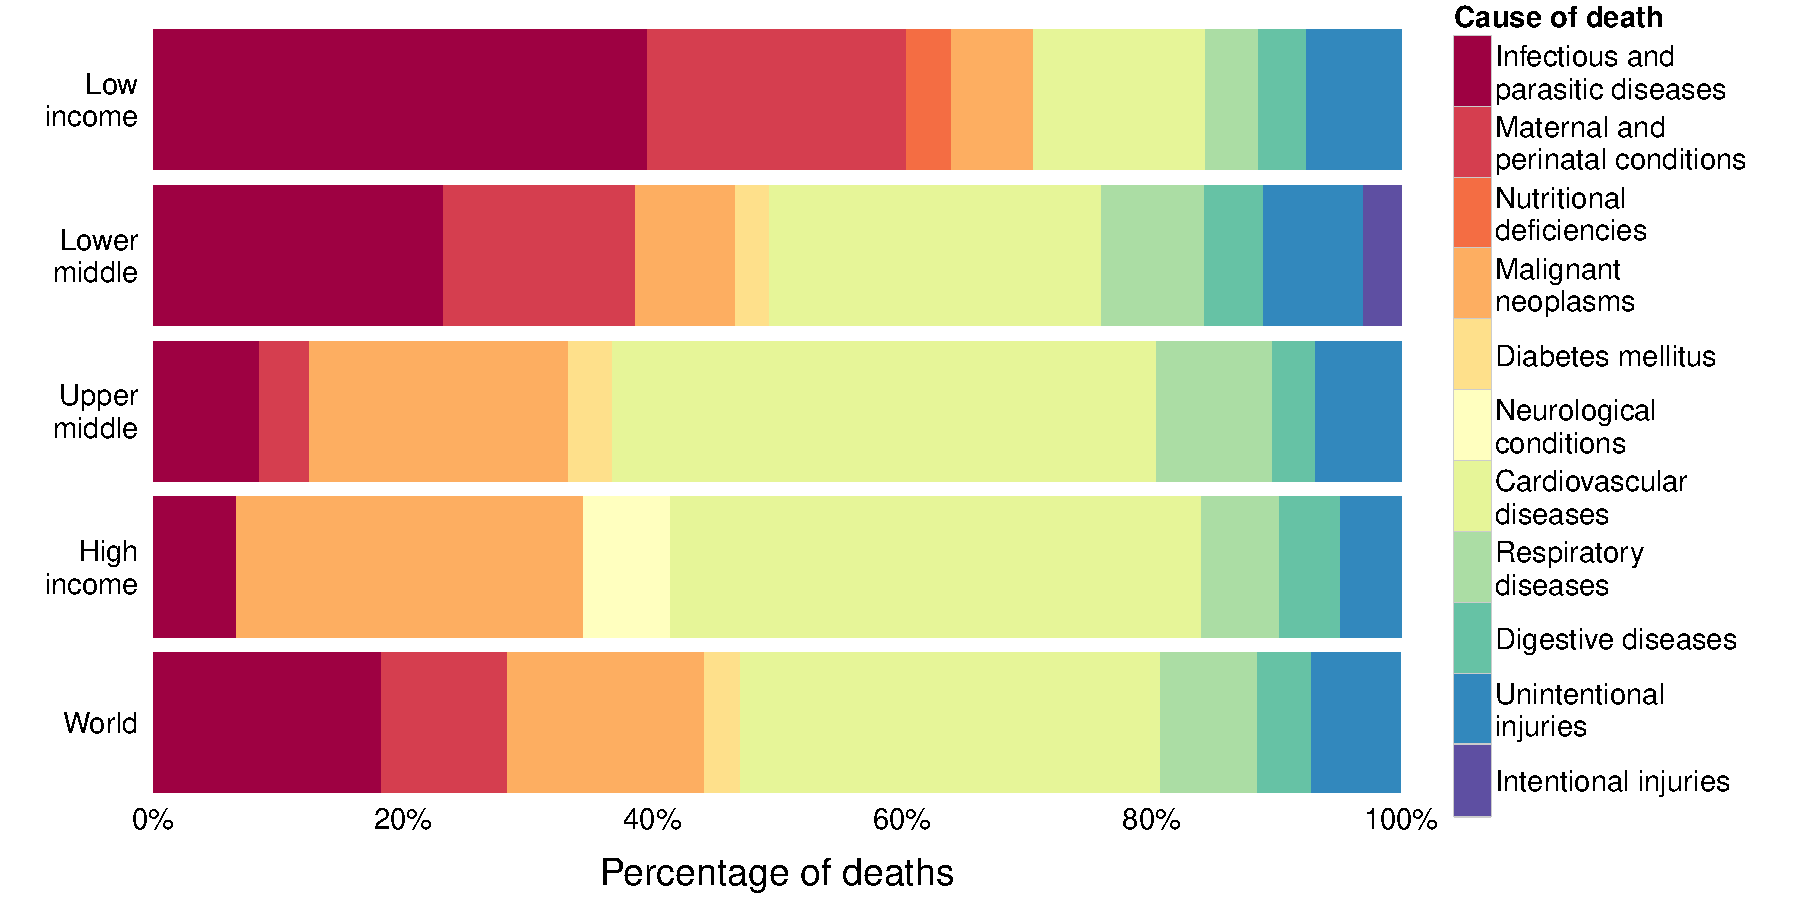
\includegraphics[width=\maxwidth]{figures/R/who-deaths/topCauses-who-deaths_top-causes-1} \caption[Relative frequencies of death causes in 2012 by World Bank income groups]{Relative frequencies of death causes in 2012 by World Bank income groups. Binning is based on Gross National Income (GNI) per capita and the thresholds are \$1'045 or less for low income, \$1046 to \$4125 for lower-middle, \$4126 to \$12745 for upper-middle and \$12746 or more for high income economies. The data was obtained from the \cite{WHO2012}.}\label{fig:who-deaths_top-causes}
\end{figure}


\end{knitrout}

\newcommand{\knitrTotalDeathsTwelve}{58.3 million}

\newcommand{\knitrPercentageDeathsTwelveHigh}{20.1\%}
\newcommand{\knitrPercentageDeathsTwelveLow}{14\%}
\newcommand{\knitrPercentageDeathsTwelveLmid}{36.5\%}
\newcommand{\knitrPercentageDeathsTwelveUmid}{29.4\%}

\newcommand{\knitrPercentDeathsTwelveLowInfect}{39.6\%}
\newcommand{\knitrPercentDeathsTwelveLowPerinat}{20.8\%}
\newcommand{\knitrPercentDeathsTwelveLmidInfect}{23.3\%}
\newcommand{\knitrPercentDeathsTwelveLmidCardio}{26.5\%}
\newcommand{\knitrPercentDeathsTwelveUmidInfect}{8.5\%}
\newcommand{\knitrPercentDeathsTwelveHighInfect}{6.7\%}
\newcommand{\knitrPercentDeathsTwelveWorldInfect}{18.3\%}
\newcommand{\knitrPercentDeathsTwelveWorldCardio}{33.7\%}


Despite development of means to treat and prevent many previously devastating diseases, infectious pathogens remain a serious threat to global health. In 2012, an estimated total of \knitrTotalDeathsTwelve{} people died (\knitrPercentageDeathsTwelveHigh{} in high, \knitrPercentageDeathsTwelveUmid{} in upper-middle, \knitrPercentageDeathsTwelveLmid{} in lower-middle and \knitrPercentageDeathsTwelveLow{} in low income countries). Figure \ref{fig:who-deaths_top-causes} partitions the total death count into World Bank income groups and causes. In low income countries, infective diseases are the most prevalent cause of death (\knitrPercentDeathsTwelveLowInfect{}), followed by maternal and perinatal complications with substantial margin (\knitrPercentDeathsTwelveLowPerinat{}). In lower middle income countries, cardiovascular conditions catch up (\knitrPercentDeathsTwelveLmidCardio{}), but are still almost matched in frequency by infectious diseases (\knitrPercentDeathsTwelveLmidInfect{}). In upper middle (\knitrPercentDeathsTwelveUmidInfect{}) and high income countries (\knitrPercentDeathsTwelveHighInfect{}), the importance of infectious disease while weakened remains accountable for a significant number of deaths. Globally, infectious diseases are the second most frequent cause of death (\knitrPercentDeathsTwelveWorldInfect{}), even more prevalent than all forms of cancer combined (\knitrPercentDeathsTwelveWorldCancer{}) and only preceded by cardiovascular diseases (\knitrPercentDeathsTwelveWorldCardio{}).

\begin{knitrout}
\definecolor{shadecolor}{rgb}{0.969, 0.969, 0.969}\color{fgcolor}\begin{figure}
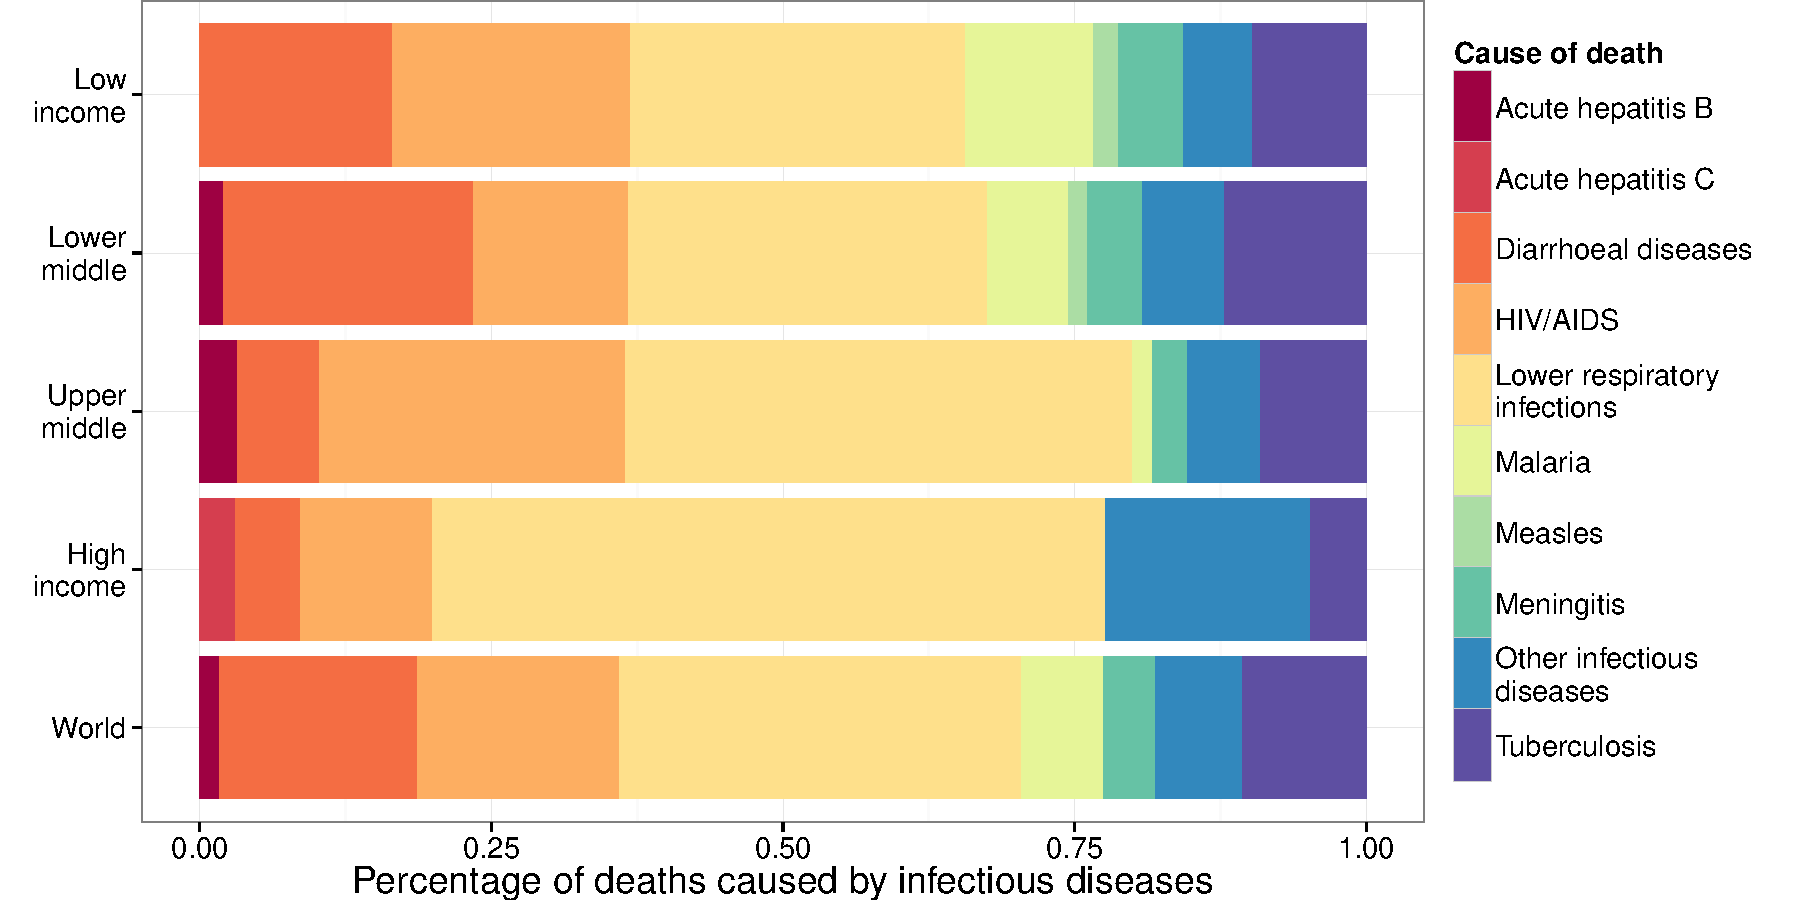
\includegraphics[width=\maxwidth]{figures/R/who-deaths/byDisease-who-deaths_by-disease-1} \caption[Relative frequencies deadly infectious diseases for 2012 by World Bank income groups]{Relative frequencies of deadly infectious diseases for 2012 by World Bank income groups. Binning is based on Gross National Income (GNI; see figure \ref{fig:who-deaths_top-causes}). The data was obtained from the \cite{WHO2012}.}\label{fig:who-deaths_by-disease}
\end{figure}


\end{knitrout}

\newcommand{\knitrPercentageInfectTwelveWorldLRI}{34.5\%}
\newcommand{\knitrPercentageInfectTwelveHighLRI}{57.7\%}
\newcommand{\knitrPercentageInfectTwelveUmidLRI}{43.5\%}
\newcommand{\knitrPercentageInfectTwelveLmidLRI}{30.8\%}
\newcommand{\knitrPercentageInfectTwelveLowLRI}{28.7\%}
\newcommand{\knitrPercentageInfectTwelveHighDiarr}{5.6\%}
\newcommand{\knitrPercentageInfectTwelveUmidDiarr}{7\%}
\newcommand{\knitrPercentageInfectTwelveLmidDiarr}{21.4\%}
\newcommand{\knitrPercentageInfectTwelveLowDiarr}{16.6\%}
\newcommand{\knitrPercentageInfectTwelveWorldAIDS}{17.3\%}
\newcommand{\knitrPercentageInfectTwelveWorldDiarr}{16.9\%}
\newcommand{\knitrPercentageInfectTwelveHighAIDS}{11.3\%}
\newcommand{\knitrPercentageInfectTwelveUmidAIDS}{26.2\%}
\newcommand{\knitrPercentageInfectTwelveLmidAIDS}{13.3\%}
\newcommand{\knitrPercentageInfectTwelveLowAIDS}{20.4\%}


Focusing only on deaths caused by infectious disease, lower respiratory infections are most frequent (for each income region individually, low to high: \knitrPercentageInfectTwelveLowLRI{}, \knitrPercentageInfectTwelveLmidLRI{}, \knitrPercentageInfectTwelveUmidLRI{} and \knitrPercentageInfectTwelveHighLRI{} as well as worldwide: \knitrPercentageInfectTwelveWorldLRI{}; cf. figure \ref{fig:who-deaths_by-disease}). Diarrhoeal diseases and \cgls{hiv}\slash \cgls{aids} are the next most common worldwide (\knitrPercentageInfectTwelveWorldDiarr{} and \knitrPercentageInfectTwelveWorldAIDS{}, respectively) where diarrhea is more prevalent in lower income regions (\knitrPercentageInfectTwelveLowDiarr{} and \knitrPercentageInfectTwelveLmidDiarr{} versus \knitrPercentageInfectTwelveUmidDiarr{} and \knitrPercentageInfectTwelveHighDiarr{}), while \cgls{hiv}\slash \cgls{aids} plays a major role irrespective of income region (low to high: \knitrPercentageInfectTwelveLowAIDS{}, \knitrPercentageInfectTwelveLmidAIDS{}, \knitrPercentageInfectTwelveUmidAIDS{} and \knitrPercentageInfectTwelveHighAIDS{}).

Dealing with highly virulent pathogens and preventing their spreading requires a multi-pronged approach. First and foremost, etiology and routes of transmission have to be understood. Knowledge of vectors and natural reservoirs is of great importance as a first line of defense. In the case of plague, for example, insecticides killing fleas were successfully used as a prophylactic measure, as was controlling rat populations \citep{Barnes1990}. Sanitary precautions including purification of drinking water, cocking foods well and the usage of disinfectants prevent initial infection, while measures such as sewage treatment, hand washing and wearing face masks help limiting spread among humans. Vaccination is the most important preventive measure. Exposing the immune system to a foreign antigen in a controlled manner artificially induces immunity. Among the great successes of widespread vaccination efforts is the global eradication of smallpox through a coordinated initiative lead by the World Health Organization in the 1970's.

Post-infection therapies include symptomatic treatments, as well as anti-in\-fec\-tive drugs. Antibiotics exploit differences in proteomes between host and pathogen to selectively disable the invader with minimal toxicity to the host. This approach has been tremendously successful throughout most of the 20th century, leading to widespread application and prompting development of resistance towards the commonly used compounds. Adding to the severity of the problem is a lack of discovery of new drugs. No new class of anti-bacterial agents has been found since 1987, causing big pharmaceutical companies to withdraw from the area. The remaining research is mainly focused on improving on existing drugs, leading to a weak product pipeline, especially for the treatment of gram-negative bacteria \citep{Silver2011}. In its first global study on anti-microbial resistance, the \citet{WHO2014} notes:

\begin{quote}
\cGls{amr} within a wide range of infectious agents is a growing public health threat of broad concern \ldots A post-antibiotic era—-in which common infections and minor injuries can kill—-far from being an apocalyptic fantasy, is instead a very real possibility for the 21st century.
\end{quote}

An alternative to pathogen directed search lies in targeting the set of host proteins necessary for infection. Many intracellular parasites subvert cellular functions to gain entry via host-mediated processes such as endocytosis. Upon entry, they move to a suitable niche and rely on host resources for proliferation. Challenges include evading host-cell defense mechanisms, generating sufficient space for replication, nutrient acquisition and keeping the host alive as long as possible, most of which require complex interactions between invader and host-based mechanisms. Finally, exiting the host cell again requires the parasite to successfully insert itself into existing signaling pathways \citep{Leiriao2004}.

\cGls{hdt} offer an escape from the conundrum of wanting to combat but not wanting to select for the surviving microbial parasites. The major challenge under this regimen is finding infectome components that are nonessential for cell survival, as orthogonality of host and infectant can no longer be exploited. Proving feasibility of the approach, \citeauthor{Czyz2014} screened a library of 640 compounds already approved by the United Stated Food and Drug Administration (USFDA or short FDA) for inducing resistance to four intracellular pathogens (\textit{Coxiella burnetii}, \textit{Legionella pneumophila}, \textit{Brucella abortus}, and \textit{Rickettsia conorii}). They found multiple drugs, not classified as antibiotics, that successfully inhibited intracellular bacterial growth while entailing only limited toxicity to THP-1 host cells. \citeauthor{Prussia2011} review the usage of genome-wide screens to study host-pathogen interactions (for \cgls{hiv} and influenza) which in turn serve as basis for rational identification of drug targets for novel host-directed antivirals. \nocite{Hawn2015}

A detailed understanding of the human infectome is of crucial importance to the development of \cgls{hdt} and may even benefit the development of new anti-microbial agents. Feasibility of systematic loss of function screens using \cgls{rna} interference methodology offers a unique opportunity to investigate complex cellular networks, making this an ideal tool for laying groundwork in combating infectious diseases. Of great importance, however, is ensuring reproducibility and comparability of such datasets, as well as ready availability to the scientific community.

Created to tackle such issues, InfectX and TargetInfectX are two successive \cgls{rtd} projects funded by SystemsX, the Swiss initiative for systems biology, contracted with identification and study of the human infectome for a set of bacterial (\textit{Bartonella henselae}, \textit{Brucella abortus}, \textit{Listeria monocytogenes}, \textit{Salmonella} typhimurium and \textit{Shigella flexneri}) and viral pathogens (adenovirus, rhinovirus and \textit{Vaccinia virus}). The central effort of generating kinome- and genome-wide \cgls{sirna} screens for each of the investigated pathogens and capturing image data followed by computational image analysis is carried out by an interdisciplinary consortium of research groups spanning the Universities of Basel and Z\"urich, the Swiss Federal institute of Technology (ETH Z\"urich), as well as the Pasteur Institute.

A wealth of data is easily generated by running computational feature recognition at single cell resolution on microscopic images which subsequently calls for sophisticated statistical analysis in order to expose biologically relevant information. This master thesis explores the single cell feature space, provides software to handle such datasets and attempts to employ \cglspl{glm} for comparing \cgls{sirna}-knockdown experiments and identifying discriminatory features. Following this introductory part, chapter 2 will provide the necessary biological background, covering microbial infection mechanisms, a description of each pathogen in terms of physical characteristics, diseases caused, pathogenesis and epidemiology, as well as giving an introduction on \cgls{rna} interference, including molecular mechanism, biological function and several applications alongside methodological caveats. Chapter 3 reviews InfectX data collection, detailing experimental setup, image acquisition, data processing and image analysis, as well as qualitatively describing the available datasets.

An R package called singleCellFeatures was developed to facilitate working with single cell feature datasets, the specifics of which are detailed in chapter 4. Beginning with a motivational example, the importance of efficient computation and data representation is highlighted and the R package is described in terms of developed S3 classes as well as data fetching, caching, manipulation and analysis routines. Finally, chapter 5 introduces \cglspl{glm}, \cglspl{pmm}, deliberates several normalization approaches and concludes with some analysis results along with a discussion of unresolved issues.


\chapter{Biological Background}

In order to better understand infectious diseases from a cell biological standpoint, this chapter reviews the current state of knowledge surrounding both bacterial and viral entry mechanisms. A sweeping overview of epidemiology and pathogenesis for several specific bacterial (\textit{Bartonella henselae}, \textit{Brucella abortus}, \textit{Listeria monocytogenes}, \textit{Salmonella enterica} and \textit{Shigella flexneri}), as well as viral parasites (adenoviruses, rhinoviruses and \textit{Vaccinia virus}) is given and the chapter concludes with a look at RNA interference as this mechanism is a cornerstone of genome-wide knockdown experiments.

\section{Microbial Host-Cell Infection}

Multi-layered keratinized skin is impenetrable for almost all microbial parasites. Instead they either require breaches such as cuts, scratches, puncture wounds and arthropod bites, or environmental interfaces which offer less impervious protection. Examples include respiratory, gastrointestinal and urogenital tracts, which all contain segments where only a single layer of epithelial cells has to be overcome. Although often protected by chemical defense mechanisms (acidity of the stomach and urogenital tract, as well as microbicidal factors in mucous secretions in the respiratory tract and small intestine), combined with frequent flushing (urination, peristalsis and the coordinated beating of cilia), some microbes have adapted to survive these hostile environments.

For extracellular pathogens to successfully colonize epithelial linings, they must avoid being removed by cleansing mechanisms of the host. Many bacteria accomplish this by expressing adhesins, protein complexes that recognize and bind to specific host-cell receptors, providing host and tissue tropism. Bacterial pili serve to extend reach and penetrate mucous secretions and therefore often carry adhesins. Enteropathogenic \textit{Escherichia coli} have extended this scheme by injecting their own receptor protein \glsrev{tir} through the \glsrev{t3ss} into the host cell to which it then attaches. This has the additional advantage that the intracellular domain of \gls{tir} can be used to modify host cell behavior \citep{Alberts2008}.

The outside of many epithelial barriers is covered in natural bacterial flora and crossing over into sterile cavities has the advantage of not having to compete with organisms well accustomed to that particular niche. Furthermore, intracellular pathogens are no longer accessible to antibodies and phagocytic cells and have a nutrient rich environment at their disposal. Mechanisms for entering host cells are described in the following sections.

\subsection{Viral Infection Mechanisms}

The first step of any viral entering sequence is binding to the target surface. This can be mediated by attachment factors which simply serve to concentrate the virions on the cell membrane or by virus receptors, which additionally act as communicators between host and pathogen. Common attachment factors include glycosaminoglycan chains and sialic acids and are comparatively unspecific. Glycoprotein spikes on enveloped and capsid proteins of non-enveloped viruses provide host specificity by binding cellular receptors. Mostly these cellular receptors serve other purposes which are exploited for infection. Binding affinity for individual interactions may be weak but aggregation of multiple interactions provide virtually irreversible avidity \citep{Smith2012}.

\paragraph{Viral import.}
For viral cell entry, different strategies exist. Enveloped viruses can either directly fuse with the plasma membrane (e.g. \gls{hiv}) or be endocytosed by the host cell (e.g. influenza), while non-enveloped viruses either create a pore and directly inject their genome into the cytosol (e.g. polio virus) or are endocytosed (e.g. adenovirus). Endocytosis has major advantages over alternative strategies. Reaching its replicatory niche within the host cell is a difficult task for a microorganism having no means of locomotion and hijacking the endocytic system solves this problem elegantly. Furthermore, maturation of endosomes provides precise environmental cues to the invader for triggering uncoating and release. Both fusion with the cell membrane and injection of viral material into the cytosol leaves back traces of infection to be detected by the immune system. Being completely engulfed by the host, however, the intruders leave back no telltale traces. Additionally, lytic membrane penetration techniques are not as problematic to the host if only applied inside an endosome as opposed to the plasma membrane.

Endocytic viruses trigger uptake either in a receptor mediated fashion (clathrin, caveolin or lipid raft dependent) or via non-specific macropinocytosis. The clathrin pathway is most widely used, for example by rhinoviruses, some adenoviruses, and coronaviruses and presents with characteristic invaginations, termed \glspl{ccp}. The inwards facing pockets are subsequently pinched off by the membrane scission proteins dynamin-1 and dynamin-2, releasing clathrin-coated vesicles into the cytosol. Caveolin-mediated endocytosis is though to be a more tightly regulated and low capacity pathway but is nevertheless exploited by several virus species, including picornaviruses and some retroviruses. Caveola formation is lipid raft dependent and recruitment of caveolin yields 50--70 nm flask-shaped pockets which are closed off by dynamin action. A lipid raft dependent, caveolin independent pathway has been described in simian virus 40 infection, but remains poorly understood. Lastly, larger virions such as poxviruses or herpesviruses initiate macropinocytosis, a mechanism typically employed by the cell for non-specific uptake of extracellular particles. An actin dependent membrane ruffling leads to formation of a lamellipodium which folds back onto the plasma membrane, enclosing an extraluminal volume and thus creating a macropinosome.

\begin{figure}
  \centering
  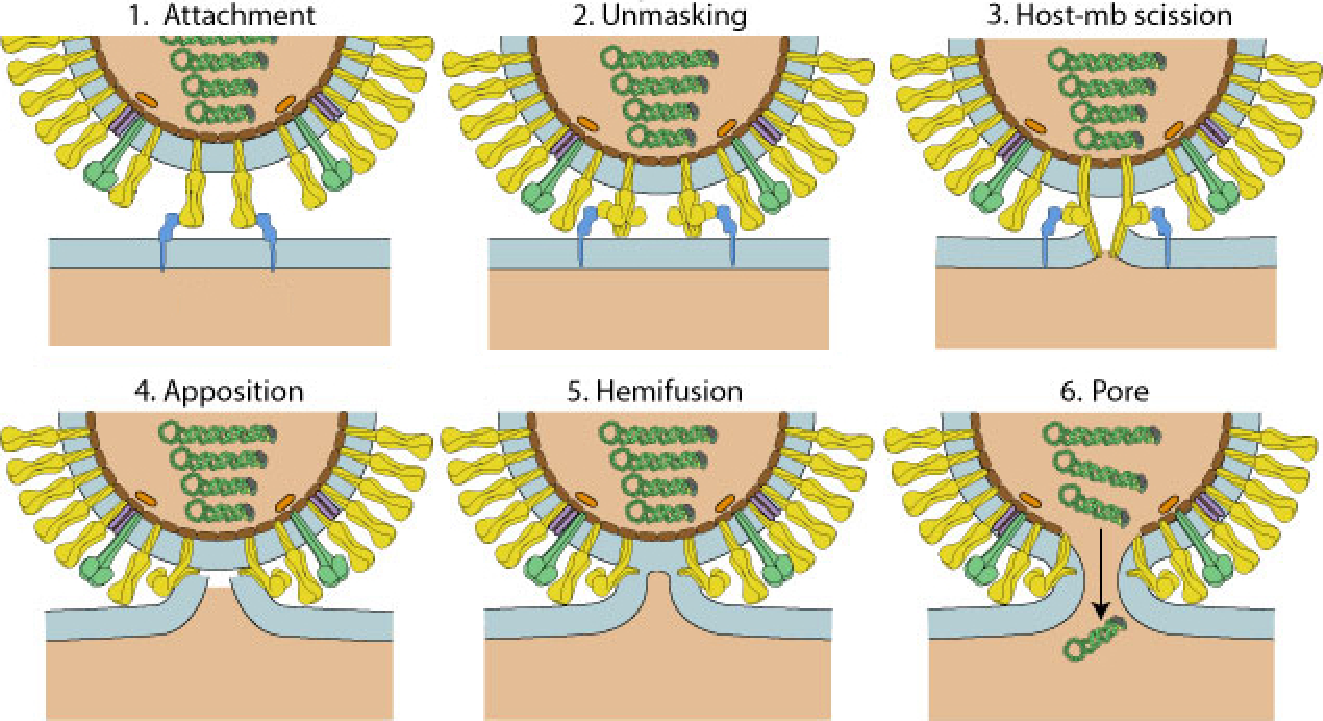
\includegraphics[width=0.95\textwidth]{virus-membrane-fusion}
  \caption[A generalized view of the steps necessary for viral--cellular membrane fusion]{A generalized view of the steps necessary for viral--cellular membrane fusion. In pre-fusion conformation, fusion proteins have their hydrophobic fusion moieties tucked away. Upon attachment (1), they are unmasked (2), interact with the target membrane and ultimately penetrate it. Conformational change in fusion proteins induces membrane scission (3) and forces the two bilayers into close proximity (4), yielding a state of hemifusion (5). Finally a fusion pore is formed (6), stabilized by the post-fusion conformation which is lower in energy than the pre-fusion state. Adapted from \cite{Hulo2011}}
  \label{fig:virus-membrane-fusion}
\end{figure}

Upon endocytic uptake, viral pathogens need to uncoat and eject their genetic material into the cytosol, as soon as their replicatory niche is reached. Escape timing is a critical issue, as late endosomes finally turn into lysosomes, capable of digesting their contents. Many enveloped viruses employ fusion mechanisms, which can be classified as type I or type II. For both types, increasing acidity associated with endosome maturation, initiates membrane fusion. Type I fusion proteins are forced into a metastable conformation prior to being added to the viral envelope and low pH triggers a conformational change to a state of lower energy. The energy released is used to force the two membranes close together resulting in their fusion (see figure \ref{fig:virus-membrane-fusion}). In type II fusion proteins, the critical transformation is not a conformational change but one in quaternary structure.

Non enveloped viruses cannot fuse with host membranes and have developed alternative approaches such as lysis (e.g. adenovirus) or ejecting their genome through pore-forming complexes (e.g. reovirus). Polyomaviruses need to pass through the \gls{er} because they rely on \gls{er} localized proteins to uncoat their capsid. For export from the \gls{er} into the cytosol, they exploit the \gls{erad} pathway, which serves as export mechanism for misfolded proteins from the endoplasmic reticulum to be degraded by proteasomes.

\renewcommand{\arraystretch}{1.5}

\begin{table}
  \centering
  \caption[The Baltimore classification scheme for viruses]{The Baltimore classification scheme is based on diversity of genetic system that have evolved in viruses. For each group, a selection of virus families capable of infecting humans, is provided, along with whether the virions are enveloped and the location of their replicatory niche. The data was obtained from \cite{Hulo2011}}
  \label{tab:baltimore-classification}
  \footnotesize
  \begin{tabular}{c|l|l|c|c}
    & Genome based class & Examples & Enveloped & Replication site \\
    \hline \multirow{4}{*}{\begin{sideways}DNA viruses\end{sideways}} &
    \multirow{2}{*}{Group I: dsDNA} &
    \textit{Adenoviridae} &
    no & nucleus \\
    \cline{3-5} &
    & \textit{Poxviridae} &
    yes & cytoplasm \\
    \cline{2-5} &
    \multirow{2}{*}{Group II: ssDNA(+)} &
    \textit{Parvovirinae} &
    no & nucleus \\
    \cline{3-5} &
    & \textit{Anelloviridae} &
    no & nucleus \\
    \hline \multirow{6}{*}{\begin{sideways}RNA viruses\end{sideways}} &   
    Group III: dsRNA &
    \textit{Reoviridae} &
    no & cytoplasm \\
    \cline{2-5} &
    \multirow{3}{*}{Group IV: ssRNA(+)} &
    \textit{Coronaviridae} &
    yes & cytoplasm \\
    \cline{3-5} &
    & \textit{Picornaviridae} &
    no & cytoplasm \\
    \cline{3-5} &
    & \textit{Hepeviridae} &
    no & cytoplasm \\
    \cline{2-5} &
    \multirow{2}{*}{Group V: ssRNA(-)} &
    \textit{Filoviridae} &
    yes & cytoplasm \\
    \cline{3-5} &
    & \textit{Paramyxoviridae} &
    yes & cytoplasm \\
    \hline \multirow{2}{*}{\begin{sideways}Retro\end{sideways}} &   
    Group VI: ssRNA(+)-RT &
    \textit{Orthoretrovirinae} &
    yes & nucleus \\
    \cline{2-5} &
    Group VII: dsDNA-RT &
    \textit{Hepadnaviridae} &
    yes & nucleus
  \end{tabular}
\end{table}

\paragraph{Replication.}
In contrast to larger intracellular parasites that carry the genetic information required for sustaining their own metabolism and replication, viral pathogens typically rely almost exclusively on host machinery. Furthermore, viruses have developed strategies for interfering with host transcription and translation in order to promote synthesis of viral proteins at the expense of host gene expression. Even modulation of the host cell cycle is not uncommon, as some DNA viruses (including adenoviruses) are able to trigger a G1 to S phase transition, yielding an increased concentration of active DNA polymerase, while other species are capable of inducing a G2/M arrest, which again provides an optimized environment for those viruses. Further virus--host interactions include regulation of apoptosis, immune response modulation and interferon signaling.

The remarkable diversity of genomic systems employed by viruses is captured by a classification system devised by \cite{Baltimore1971}. Table \ref{tab:baltimore-classification} lists the 7 types of viral genomes alongside examples of human viruses for each group, as well as whether those viruses are enveloped and where they replicate. Consequently, requirements for replication, transcription and translation vary widely among the different groups of viruses and due to the resulting mechanistic heterogeneity, viral propagation is not further explored within this general section. An excellent overview is provided by the online database of \citeauthor{Hulo2011}.

\paragraph{Viral export.}
The final stage of the viral life-cycle is concerned with virion assembly and exiting the host cell. Again, many strategies exist. Some nuclear replicating viruses (such as polyomaviruses) assemble their capsid proteins within the nucleus, requiring their structural proteins to target the nucleus via \glspl{nls} and leave the nucleus by disrupting the nuclear envelope, while others have their genome exported via nuclear pores and assemble progeny virions in the cytoplasm. Some cytoplasmic viruses (including poxviruses) replicate within special structures called viral factories or viroplasms, which increase efficiency of assembly and packaging and provides protection from host defense mechanisms. Other cytoplasmic viruses localize to organelles such as the \gls{er} (e.g. flaviviruses) where they are assembled and enter the secretory pathway via the Golgi apparatus. For intracellular motility, large virions such as poxviruses or herpesviruses have to rely on microtubule dependent transport whereas particles smaller than 20 nm can freely diffuse within the cytosol.

Once the host cell resources are depleted and replication is completed, progeny virions trigger their release. Viral shedding may occur via cell lysis, apoptosis, exocytosis or virion budding. Most non-enveloped and few enveloped viruses disrupt the plasma membrane with lytic viroproteins leading to cell death and release of cytoplasmic contents. While many viruses inhibit  apoptosis, typically employed as a host defense measure, some (including hepeviruses and lentiviruses) have been implicated in exploiting this mechanism for expulsion and possibly subsequent infection of macrophages. Exocytosis and virion budding are two release strategies that are non-lethal to the host cell. Enveloped viruses acquire host-derived membrane either within the cell, typically at \gls{er} or Golgi exit sites or directly from the plasma membrane. In the latter case, envelopment coincides with host exit, whereas in the former case, virions are expelled via fusion of exocytic vesicles with the plasma membrane.

\subsection{Bacterial Entry Mechanisms}

Due to the much larger size of bacterial pathogens, endocytosis is not a feasible mechanism for entry. Phagocytosis, however can deal with uptake of particles this large. While phagocytosis is a function usually only available to macrophages, some bacteria have evolved mechanisms of inducing phagocytosis in other cell types. Species explicitly targeting macrophages, such as \textit{Mycobacterium tuberculosis} and \textit{Legionella pneumophila}, have to be able to escape phagosomes or deal with resisting digestion.

Two recurring patterns for inducing phagocytosis in non-phagocytic cells have been described as the zipper mechanism, encountered in \textit{Yersinia pseudotuberculosis} and \textit{Listeria monocytogenes} and the trigger mechanism used by \textit{Salmonella enterica} and \textit{Shigella flexneri}. Not all entry strategies can be assigned to these two classes and several additional, unrelated pathways have been investigated.

\begin{figure}
  \centering
  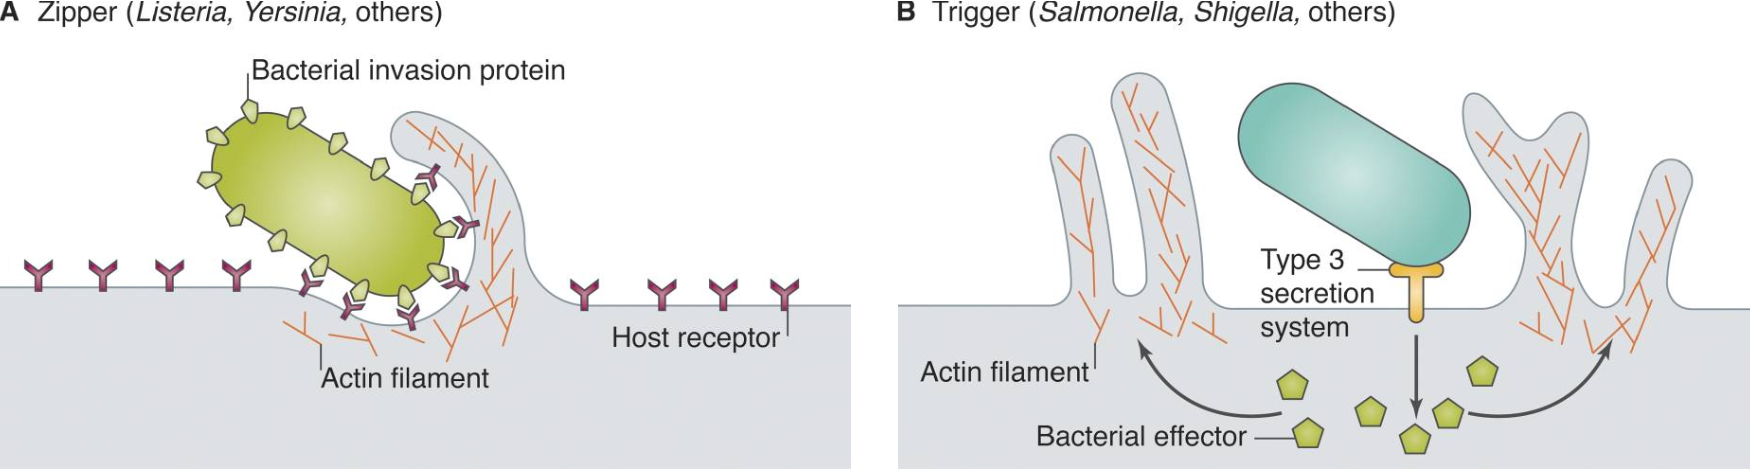
\includegraphics[width=0.6\textwidth]{zipper-trigger}
  \caption[Zipper and trigger mechanisms for bacterial host-cell entry]{Both the zipper (A) and trigger mechanisms (B) are actin dependent and lead to phagocytosis by usually non-phagocytic host cells. Zippering bacteria display an invasion protein on their surface that recruits actin filaments via a host receptor, while triggering bacteria inject an effector into the host cytosol via a type III secretion system leading to uptake. \citep{Haglund2011}}
  \label{fig:zipper-trigger}
\end{figure}

\phantomsection
\label{zipper-mechanism}

\paragraph{Zipper Mechanism.}
The first step for zippering bacteria is binding to target cell receptors by expressing adhesins. \textit{Y. pseudotuberculosis} displays invasins on its cell surface, capable of interacting with \textbeta$_1$ integrins, while \textit{L. monocytogenes} uses internalin A, a protein that binds E-cadherin. In both settings, a downstream signaling cascade leads to actin polymerization via recruitment of an \glsrev{arp-2-3} complex and \glsrev{rac-1}, yielding a phagocytic cup.

Cadherin and integrins are usually involved in anchoring cell junctions and the host cell is fooled into thinking, a neighboring cell is initiating formation of such a junction. Responding by recruiting actin at the site of bacterial attachment to cover the surface of mistaken invasion proteins leads to engulfment and phagocytosis to the bacterium. This process incurs only modest cytoskeletal rearrangements. 

\phantomsection
\label{trigger-mechanism}

\paragraph{Trigger Mechanism.}
In case of the trigger mechanism, bacterial \gls{t3ss} weakly adhere to target cell receptors (CD44 for \textit{Shigella}) and effector molecules are injected into the host cytosol through a pore formed by \glsrev{sip} or \glsrev{ipa} proteins. These induce major actin rearrangements that result in localized ruffling of the plasma membrane and subsequent swallowing of the bacterium.

Early in \textit{Shigella} entry, VirA, secreted through the \gls{t3ss} causes local destabilization of microtubules by binding to \textalpha/\textbeta-tubulin heterodimers. This in turn stimulates \glsrev{rac-1} activity, \glsrev{cdc-42} recruitment and subsequent \gls{arp-2-3} activation leading to protrusions formed by actin filaments. \Gls{ipa}C recruits the Src tyrosine kinase further enhancing actin dynamics. Upon closing of the phagocytic pocket, the \gls{t3ss}-secreted protein \gls{ipa}A binds to vinculin and induces actin depolymerization.

\textit{Salmonella} inject the proteins \glsrev{sop}E and \glsrev{spt-p}, an activator/inhibitor pair for the GTPase complex \gls{rac-1}/\gls{cdc-42}, into the host cell. First, \gls{gef} activity of \gls{sop}E induces massive actin-rearrangements leading to membrane ruffling and facilitating phagocytosis, followed by GAP activity of \gls{spt-p}, restoring the inactive \gls{gdp} state of \gls{rac-1}/\gls{cdc-42} and leading to actin depolymerization. \Gls{sop}E is degraded more rapidly than \gls{spt-p}, enabling the invading pathogen to reversibly control the pathways exploited for entering.

\paragraph{Other Entry Pathways.}
In addition to trigger and zipper type uptake, other atypical mechanisms exist. Host cell entry of \textit{Brucella abortus}, for example, has been described as invasome mediated \citep{Dehio2005}. In this actin dependent process, bacteria aggregate on the cell surface and trigger their engulfment by injecting bacterial effectors into the host via \gls{t4ss}. The internalized structure is called an invasome. Actin-independent uptake albeit rare, is possible as evidenced by \textit{Campylobacter jejuni}, which have evolved a microtubule dependent invasion strategy \citep{Kopecko2001}.

\subsection{Actin-based Intracellular Motility}
\label{subsec:actin-motility}
As for large viruses, free diffusion within the cytoplasm is not possible for bacteria.

\section{Select Bacterial Pathogens}

A total of 5 bacterial pathogens were selected for study within the InfectX RTD project by SystemsX. This section shortly describes each organism in terms of microbiological features, pathogenesis, epidemiology and diseases caused in humans. For each organism, a chapter of \cite{Rolain2006} serves as basis and is augmented by one or two review article referenced in the first paragraph of each section.

\subsection{\textit{Bartonella Henselae}}

\textit{Bartonella henselae} is a short, rod shaped, unflagellated proteobacterium, phylogenetically closely related to the genus \textit{Brucella}, presenting 94.4\% 16S rRNA gene sequence homology, compared with \textit{Brucella abortus}. The Gram-negative bacillus is a facultative anaerobic, intracellular parasite and was first described in 1992. Relatively harmless for healthy humans, infections can become life threatening in immunocompromised patients, making the species an important opportunistic pathogen \citep{Anderson1997}.

\paragraph{Diseases.}
In immunocompetent humans, infection with \textit{B. henselae} can lead to a condition known as \gls{csd}. As the name suggests, most patients report being in contact with a cat and transmission often occurs through scratches and bites. Affecting primarily children and young adults (80\% are 21 or younger), the self limiting infection typically presents itself with lymphadenopathy. Most patients remain afebrile and do not report feeling ill, with low-grade fever and malaise shown in roughly 30\% of the cases. Recovery from uncomplicated \gls{csd} usually takes 2 to 6 months and requires no specific treatment.

Possible complications include Parinaud's oculoglandular syndrome (granulomatous conjunctivitis in one eye and parotid lymphadenitis on the same side), splenomegaly and hepatic or splenic abscesses, accompanied by fever, weight loss, fatigue and malaise. In 1 to 7\% of the cases, the disease spreads to the central nervous system, leading to encephalopathy, but recovery is usually rapid (within several weeks).

Infections with \textit{B. henselae} tend to have more severe consequences for immunocompromised patients, such as bacillary angiomatosis, bacteremia and endocarditis. \Gls{aids} patients suffering from \gls{csd} usually experience severe, progressive disease with infection spreading systematically and without appropriate treatement, fatal outcome. \textit{Bartonella spp.} are the only prokaryotes known to be able to induce angiogenic tumors such as bacillary angiomas, which may involve skin, respiratory or gastrointestinal epithelia, hart, liver, spleen, bone marrow, muscles, or lymph nodes. Bacteremia may lead to inflamed heart valves, usually requiring endocarditic patients to have heart valve replacement surgery.

\begin{figure}
  \centering
  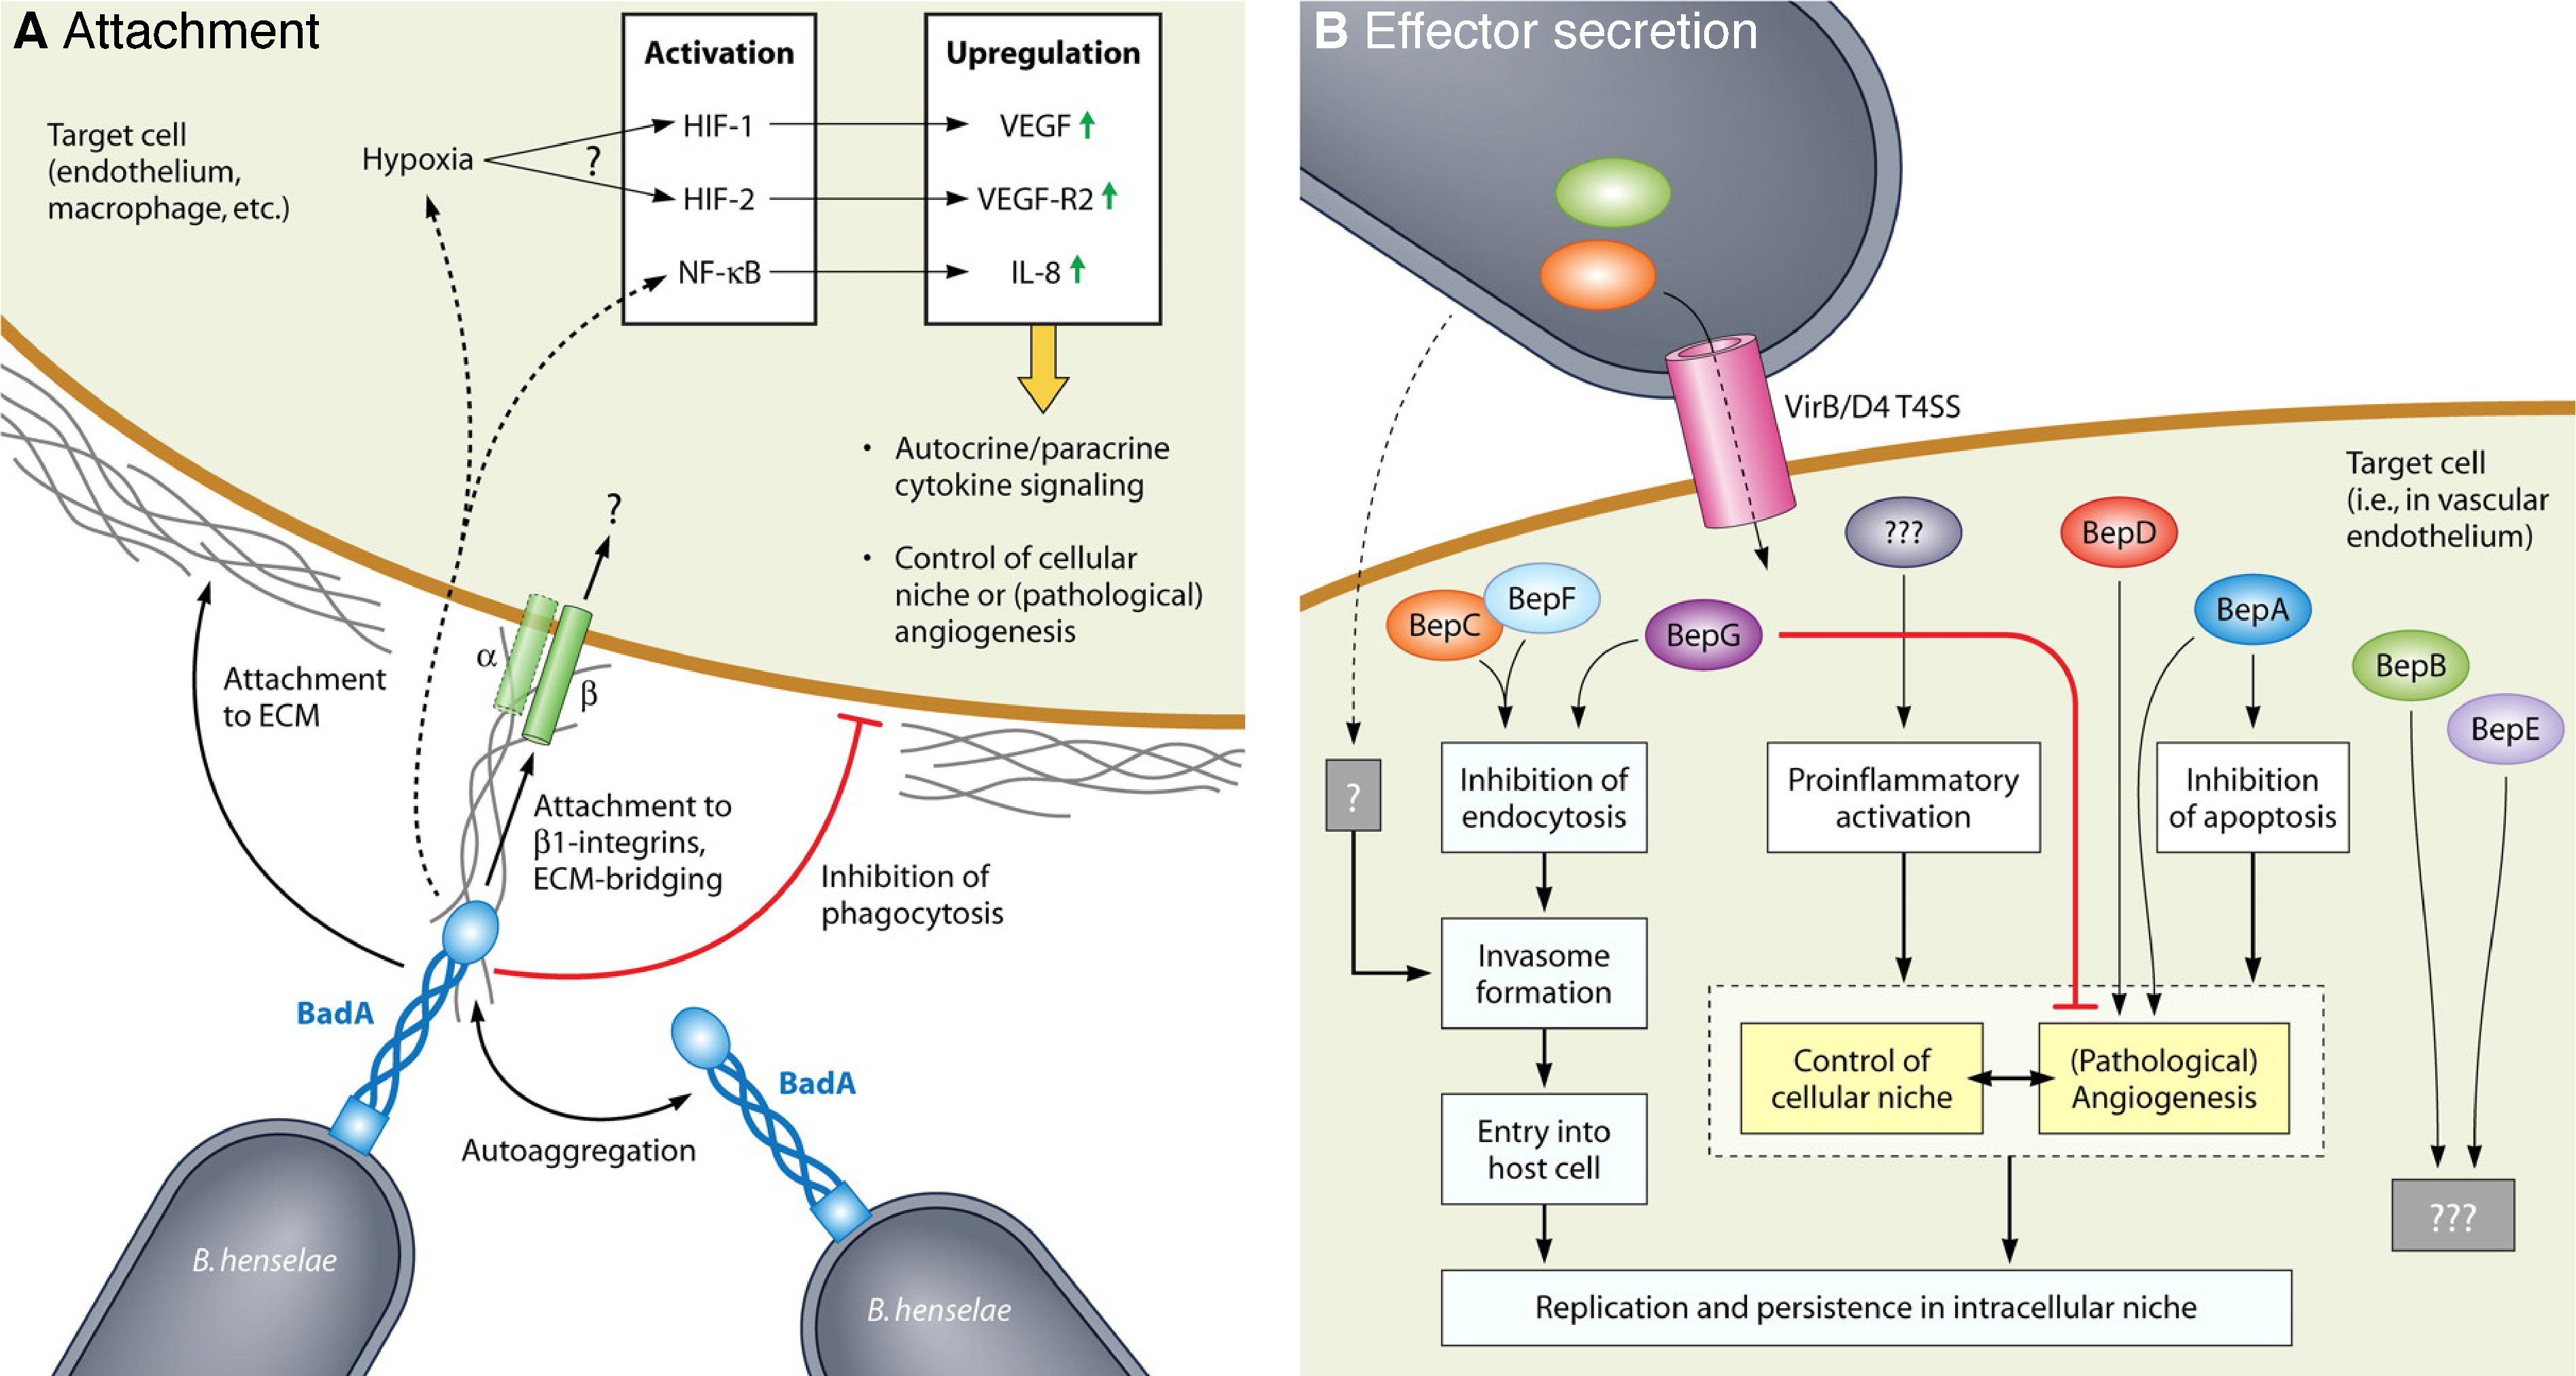
\includegraphics[width=0.75\textwidth]{bartonella}
  \caption[Replication cycle of \textit{Vaccinia viruses} for both intracellular mature and extracellular enveloped virions.]{Capsid proteins VP1 through VP4 form a pseudo $T=3$ icosahedral coat, roughly 30 nm in diameter around the RNA genome (A), which is monopartite, linear, 7.2 kp long and encodes 11 proteins \citep{Harms2012}.}
  \label{fig:bartonella}
\end{figure}

\paragraph{Pathogenesis.}
\textit{B. henselae} are capable of intracellular growth in both epithelial cells, and erythrocytes. Bundle forming type IV pili are essential for binding to target cells, making them important virulence factors. Internalization into red blood cells may be spectrin mediated and the bacterial protein deformin may also be involved. Endothelial receptors involved include \gls{icam-1} uptake is either via endocytosis or by a unique cellular structure termed an invasome.

Vasculogenesis is induced though an increased production in \gls{vegf} by infected host cells. Currently it is poorly understood how the pathogen provokes overexpression but the mechanism has been determined to be protease sensitive.

\paragraph{Epidemiology.}
The role of cats and in particular kittens, as reservoirs to \textit{B. henselae} has been firmly estabished. Infected felines are asymptomatic and show no signs of illness. Cat fleas (\textit{Ctenocephalides felis}) serve as vectors to spread the bacteria among cats and have also been suspected of infecting humans. The main path of transmission to humans however, is through scratches and bites by infected cats. \textit{B. henselae} has also been found in ticks and tick bites prior to contraction of \gls{csd} have been reported.

In the United States, 24000 cases of \gls{csd} are reported yearly, yielding 2000 hospital admissions with an estimated health care cost of \$12 million. Children are more likely to be affected (80\%) and incidence is higher in males (60\%). The seasonal pattern (occurrences higher in fall/winter) is attributed to cat mating patterns, as well as pet acquisition fluctuations.

\subsection{\textit{Brucella Abortus}}

The Danish physician David Bang first isolated \textit{Brucella abortus} in 1895 from cyetic cattle tissue, investigating a contagious disease causing abortions in cows. \textit{B. abortus} are small, unflagellated proteobacteria with a cell wall consisting of an outer layer of \gls{lps} (9 nm) and an inner layer of muramyl mucopeptide complexes (3--5 nm). The Gram-negative cocobacilli appear to have evolved from free-living, soil-dwelling species and are closely related to other human pathogens such as \textit{Bartonella} spp., based on 16S rRNA sequences. Brucella species were investigated for possible use as warfare agents in the mid 20th century by several armed forces. \citep{Atluri2011}

\paragraph{Diseases.}
Brucellosis is a human disease caused by several pathogenic \textit{Brucella} species, most importantly \textit{B. abortus}, \textit{B. melitensis}, \textit{B. canis} and \textit{B. suis}. Onset may be acute or insidious and due to protean symptoms, diagnosis based on clinical presentation alone is difficult. The febrile disease is generalized and may involve many parts of the body, including nervous, skeletal, gastrointestinal, cardiovascular, respiratory and genitourinary systems. Furthermore, as the bacteria spread to other reservoir hosts via their reproductive systems, persistence of infection is crucial to the pathogen and it comes as no surprise that brucellosis can manifest as a chronic disease in humans too.

Fever is the most consistent sign of \textit{Brucella} infection and depending on what specific organs are affected, further symptoms include asthenia, anorexia, nausea, malaise, arthritis, hepatomegaly, splenomegaly, epididymo-orchitis in males, and pulmonary manifestations such as bronchitis or pneumonia. A rare complication (less than 2\%), albeit the most lethal, is infective endocarditis. Invasion of the nervous system occurs in less than 5\% of cases and often results in meningitis or meningoencephalitis with good prognosis under antimicrobial treatment.

\begin{figure}
  \centering
  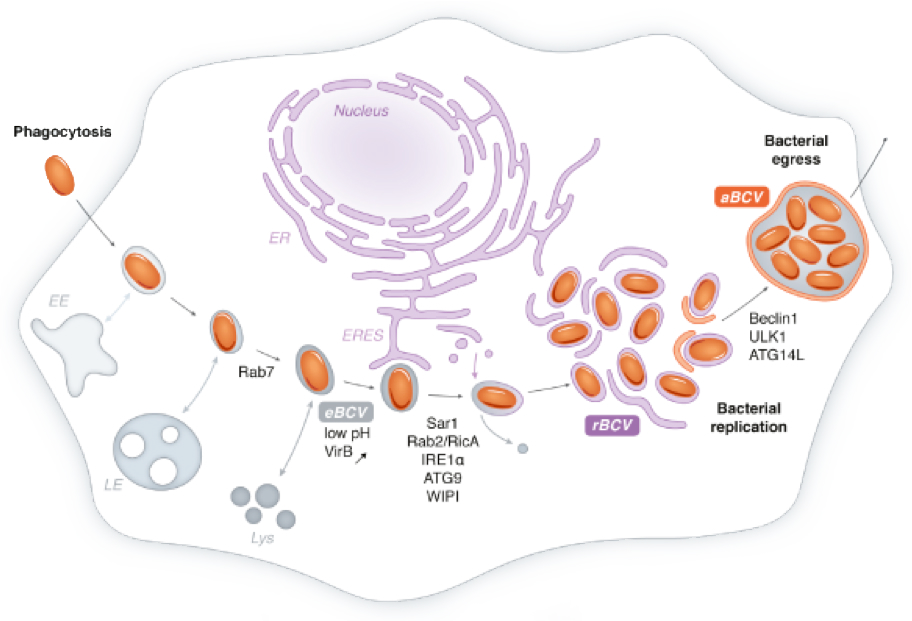
\includegraphics[width=0.95\textwidth]{brucella}
  \caption[Replication cycle of \textit{Vaccinia viruses} for both intracellular mature and extracellular enveloped virions.]{Capsid proteins VP1 through VP4 form a pseudo $T=3$ icosahedral coat, roughly 30 nm in diameter around the RNA genome (A), which is monopartite, linear, 7.2 kp long and encodes 11 proteins \citep{Celli2015}.}
  \label{fig:brucella}
\end{figure}

\paragraph{Pathogenesis.}
Host entry happens primarily via the digestive system but is also possible through the respiratory tract or skin lesions. On the gastrointestinal route, \textit{Brucella} spp. target Peyer's patches (lymphoid nodules localized towards the end of the small intestine) and must therefore pass through acidic conditions in the stomach. This is facilitated by expression of two ureases capable of hydrolyzing urea and producing a protective bicarbonate buffering system. When entering through the respiratory system, \textit{B. abortus} target alveolar macrophages which serve as access point to the lymphatic system therefore facilitating systematic spread.

In order to persist at systemic sites, both active and passive mechanisms for evading the immune system are in place. \Gls{lps} of the outer cell wall disguises the bacteria from \glspl{tlr} and expression of two proteins containing \gls{tir-1} domains actively interferes with \gls{tlr} signaling.

Uptake by macrophages happens via phagocytosis, which is either triggered by nonopsonized bacteria through a lipid raft mediated mechanism or by opsonization. Although opsonin marked bacteria are 10-fold more likely to be ingested, the number of pathogens reaching their replicatory niche within the host cell is higher for nonopsonized bacteria. Maturation of early endosomes into lysosomes is important for successful infection as preventing acidification (through addition of bafilomycin A) or fusion with lysosomes (through suppression of the late-endosomal GTPase Rab7) interferes with bacterial replication. Nonopsonized bacteria finally become associated with rough ER and begin replication in ER derived vacuoles within the \gls{ergic}. Blocking the small GTPase Sar1 inhibits intracellular replication by preventing acquisition of \gls{cop-2} by ER-exit vesicles and the small GTPase Rab2, involved in ER--cis-Golgi traffic, is required for maximal proliferation.

Despite multiplying intra-cellularly in high numbers, host cells are kept alive and are even able to replicate despite infection. Furthermore \textit{Brucella} species are able to interfere with apoptosis, maintaining their replicatory niche, protected from immune response.

\paragraph{Epidemiology.}
Preferred natural reservoir species for \textit{B. abortus} are cattle (\textit{Bos taurus} and \textit{Bos indicus}) and almost all parts of the world are affected. The disease exists in both domestic and wild animals and is most prevalent in Mediterranean countries, North Africa, throughout the Middle East, India, Central Asia, as well as South and Central America. Zoonosis most often occurs through ingestion if unpasteurized milk products but airborne transmission is also possible, putting professionals involved in animal husbandry at risk. Vertical transmission among reservoir hosts can occur through lactation and horizontal transmission is facilitated by mating and placental discharge associated with aborted gestation. Human-to-human transmission is rare (but has been suspected to be possible via sexual intercourse), making humans dead-end hosts. As opposed to \textit{Bartonella}, immunodeficient patients do not seem to be especially susceptible towards \textit{Brucella} infections.

Worldwide, an estimated 500000 new cases of brucellosis occur annually, making it one of the most prevalent zoonoses. Although usually susceptible to combined antibiotic therapies of at least two agents (usually a tetracycline antibiotic combined with an aminoglycoside or rifampin), untreated brucellosis leads to a high degree of morbidity, leading to being classified a neglected zoonosis by the \gls{who}.

\subsection{\textit{Listeria Monocytogenes}}

The short, Gram-positive bacilli are non-sporeforming facultative anaerobes, capable of growing in a wide temperature range (0--50\si{\degree}C) and in many different environments. Flagellation is temperature dependent with flagellin being expressed and assembled into peritrichous flagella around 20--25\si{\degree}C but not at 37\si{\degree}C. First described in 1924 by Murray after isolation from lymph glands of diseased laboratory animals, the pathogen was found to also infect humans four years later. For much of the time since, listeriosis was considered a rare zoonotic disease and did not receive much attention. It was not until the 1980s, when several food-borne listeria outbreaks caused a shift in interest towards the pathogen, which has since become a well studied facultatively intracellular parasite \citep{Farber1991}.

\paragraph{Diseases.}
Maternal and neonatal listeriosis accounts for almost half of all infections. Listeriosis in pregnancy typically manifests in bacteraemia and presents as a self-limiting febrile disease with flu-like symptoms. Many cases, however are asymptomatic and the first sign of infection is abortion or neonatal listeriosis. Maternal infection does not necessarily carry over to the fetus, especially if proper chemotherapy is administered. Perinatal incidences are divided into early and late onset (\textgreater 5 days after parturition), with former cases typically resulting in septicemia and latter cases in meningitis. While in early onset cases the predominant route of transmission is transplacental, the situation is less clear in late onset cases. Both the maternal genital tract during child birth and environmental sources have been implicated. Despite antibiotic treatment, overall mortality rates of 30--40\% are typical and prognosis for early onset disease is worse, as it is often associated with preterm birth and advanced stage of infection. 

Among adults, most cases of listeriosis occur in T-cell deficient individuals. HIV infection, for example, increases incidence 150--300 fold compared to general population control groups. Predisposing conditions include lymphoreticular neoplasms, deliberate immunosuppression (e.g. antirejection treatment after organ transplants), alcoholism and diabetes mellitus. Despite increased susceptibility caused by immunodeficiency, roughly 30\% of all infections affect immunocompetent individuals. In healthy adults, consumption of food contaminated with \textit{L. Monocytogenes} can either lead to self-limiting febrile gastroenteritis with short incubation time (\textless 24 h) or invasive listeriosis with much longer incubation periods (3--4 weeks). The systemic form of infection often manifests as bacteraemia or as a neurological infection, but can also involve endocarditis and spread to other parts of the body. Central nervous system involvement occurs in as much as 75\% of cases and either presents as meningitis or encephalitis. Mortality rates of 35--45\% have been reported for listeriosis in adults.

\begin{figure}
  \centering
  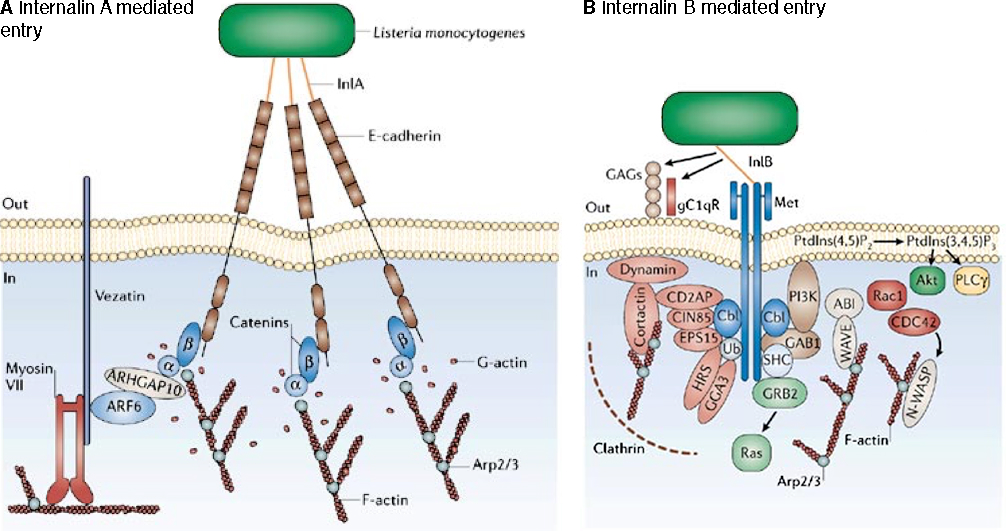
\includegraphics[width=0.8\textwidth]{listeria}
  \caption[Capsid structure and genome of rhinoviruses.]{Capsid proteins VP1 through VP4 form a pseudo $T=3$ icosahedral coat, roughly 30 nm in diameter around the RNA genome (A), which is monopartite, linear, 7.2 kp long and encodes 11 proteins (B). Figures adapted from \cite{Lebreton2015}.}
  \label{fig:listeria}
\end{figure}

\paragraph{Pathogenesis.}
The predominant entry path for \textit{L. Monocytogenes} into the human body is via the gastrointestinal tract, where Peyer's patches are targeted. The bacteria can induce cellular uptake (see section \ref{zipper-mechanism}), even by non-phagocytic host cells via expression of cell-surface associated interanlins. Upon cell entry, the phagosomal membrane is lysed, mediated by haemolysin secretion, and actin polymerization (see section \ref{subsec:actin-motility}) provides means of intracellular movement. Listerial haemolysin (listeriolysin) is acid activated with an optimum around pH 5.5, which is reached in late endosomes and membrane lysis is caused by the formation of large transmembrane pores. Growth and replication occur in the cytoplasm and adjacent cells can be entered by pushing against the plasma membrane and forming a pseudopod-like structure which in turn is taken up the neighbor. The resulting double-membrane vacuole can be escaped by cytolysis.

In an extracellular setting, haemolysins serve to rupture erythrocytes in order to generate free iron, a limiting growth factor. Furthermore the nonspecific immune system has to be evaded and haemolysins have also been shown to be cytotoxic towards leukocytes. Additionally, expression of bacterial superoxide dismutase mitigates the effect of free superoxide radicals which play an important role in killing phagocytized bacteria.

\paragraph{Epidemiology.}
Incidence of listeriosis has initially been increasing since its recognition as food-borne disease but effects of awareness and diagnostic methods are unclear. While typically long incubation periods do pose difficulties for clinical diagnosis, the number of susceptible individuals is on the rise and certain aspects modern processing and handling of foods may be beneficial for growth of \textit{L. Monocytogenes}. Disease rates of 2--15 cases per million population per year have been reported and listeriosis is among the leading case of lethal food-borne pathogen infections. Most recent data, however suggests, that incidence is decreasing again.

Due to its non-fastidious lifestyle, \textit{L. Monocytogenes} has been isolated from a wire array of ecological niches, including soil, sewage and water (both fresh water bodies and estuaries). High persistence (up to 4 years) in soil samples is problematic when contaminated manure is used as fertilizer and biofilm formation poses challenges for eradication from food processing plants. Additionally, the ability to grow in refrigerated foods and resistance towards heat treatment such as pasteurization warrant alertness and special preventive care. Many different foods have been implicated in listeriosis outbreaks, including vegetables (potatoes, radishes and celery), seafood (shrimp, crabmeat and smoked fish), diary products (soft cheese, pasteurized and unpasteurized milk) and meats (poultry, various types of sausages and pâté).

Despite high prevalence in food (studies have found 20--80\% of meat product samples and 1--10\% of diary product samples contaminated with \textit{L. Monocytogenes}), comparatively few successful infections occur. The bacteria are ingested frequently in small doses and stool sample examinations suggest that 10-70\% of investigated populations could be intestinal carriers. While the minimum infectious dose has not been settled definitively, approximations range from $10^6$ to $10^9$ bacteria.

\subsection{\textit{Salmonella} Typhimurium}
\textit{Salmonella} are non-sporulating, Gram-negative bacilli, belonging to the family Enterobacteriaceae. The motile bacteria are able to produce peritrichous flagella and diameters span 0.7 to 1.5 \textmu m while typical lengths range from 2 to 5 \textmu m. They are closely related to the genus \textit{Escherichia}, showing only 15\% chromosomal sequence disparity. Currently, two distinct species, \textit{S. bongori} and \textit{S. enterica}, within the genus \textit{Salmonella} are recognized, both of which are pathogenic towards a wide array of hosts. \textit{S. enterica} is further divided into 6 subspecies, the most relevant of which for human and domestic animal hosts being \textit{enterica}. A large number of serovars (more than 2500) for \textit{S. enterica} subsp. \textit{enterica} have been characterized and due to an originally mistaken classification as separate species, some serovars are designated with shortened names. \textit{S.} Typhimurium, therefore is shorthand for \textit{S. enterica} subsp. \textit{enterica}, serovar Typhimurium and to emphasize that Typhimurium is not a species description it is not italicized.

The first description of the genus \textit{Salmonella} dates back to an investigation into swine fever led by Salmon and Smith in 1885. The newly isolated bacterium was wrongly proposed as the etiological agent, as the disease later tuned out to be caused by a virus \citep{Fabrega2013}.

\paragraph{Diseases.}
Two distinct disease patterns are associated with \textit{Salmonella} spp. infections, typhoid fever and salmonellosis. While the former is exclusively caused by the serovars Typhi and Paratyphi, the latter is associated with several serovars, the most frequent being Enteritidis and Typhimurium, accounting for 65\% and 12\% of cases worldwide. The current and following sections will not discuss typhoid fever.

Salmonellosis is a diarrheal disease with a short incubation period of 6--24 h, followed by nausea, vomiting, loose or liquid bowel movements, abdominal cramps and fever. Clinical features are similar to those of dysentry and other gastroenteric disease and can include bloody and mucosal stool. In most cases, the infection is self-limiting and symptoms fade away within 4 to 7 days. The most common complication is bacteraemia, which presents in 5\% of cases and is more likely to develop in children, especially if malnourished, and immunocompromised individuals. Further manifestations of invasive infections include meningitis, osteomyelitis, cholangitis, pneumonia and endocarditis. While mortality in immonocompetent hosts in developed countries is as low as 0.1\%, it can increase to 77\% for \gls{hiv} positive patients in undeveloped countries.

\begin{figure}[t]
  \centering
  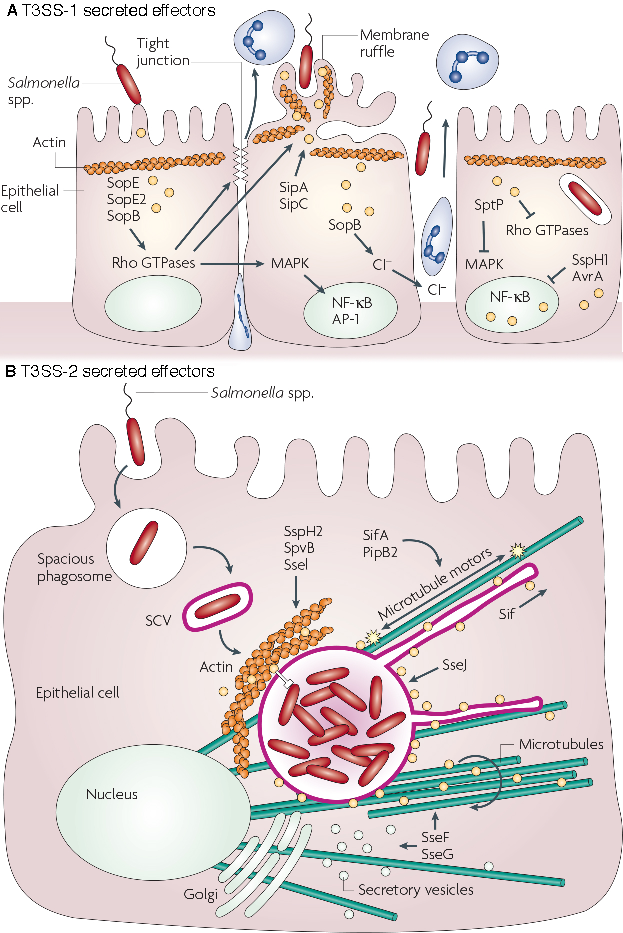
\includegraphics[width=0.7\textwidth]{salmonella}
  \caption[Capsid structure and genome of rhinoviruses.]{Capsid proteins VP1 through VP4 form a pseudo $T=3$ icosahedral coat, roughly 30 nm in diameter around the RNA genome (A), which is monopartite, linear, 7.2 kp long and encodes 11 proteins (B). Figures adapted from \cite{Haraga2008}.}
  \label{fig:salmonella}
\end{figure}

\paragraph{Pathogenesis.}
In order to reach the small intestine, ingested \textit{S.} Typhimurium first are exposed to the hostile environment of the stomach. A set of proteins, summarized as \gls{atr} helps mediate the acidic conditions and improves survival rates. The reamining bacteria subsequently reacht the small bowel and target its epithelial cells, with preference towards \gls{m-cells}. Flagellar motility enables penetration of intestinal mucus secretions and improves the chance of reaching the intestinal walls where adhesion can be established. Fimbriae are important attachment factors, capable of interaction with host-cell laminin and fibronectin and provide an initial platform for pathogen induced phagocytosis via trigger mechanism (see section \ref{trigger-mechanism}). 

\textit{S.} Typhimurium utilize two separate \gls{t3ss} systems for host-cell colonization, the first of which (\gls{t3ss}-1) mediates invasion. In addition to strengthening initial interactions attaching the pathogen to its target, the needle like structure serves as delivery mechanisms, capable of injecting effector proteins, including \gls{sop}E, \gls{sop}E2, \gls{sop}B (also known as SigD) and \gls{sip}A. \Gls{sop}E serves as \gls{gef} and activates \gls{rac-1} and \gls{cdc-42} via \acrshort{gdp}/\acrshort{gtp} exchange, which in turn initiate cytoskeletal rearrangements. \Gls{sop}E2 is a further \gls{gef}, highly homologous to \gls{sop}E and it is assumed to fill in for \gls{sop}E in \textit{Salmonella} strains missing the \gls{sop}E gene. \Gls{sop}B is a phosphatase, capable of hydrolyzing various substrates, including \gls{i13456p5}, which has been linked to intestinal fluid secretion causing diarrhea and \gls{pi45p2}, which is involved with membrane rigidity. Finally, the actin binding protein \gls{sip}A  stimulates stimulates actin polymerization and promotes membrane ruffling.

Upon engulfment, maturation of the phagosome and fusion with lysosomes have to be prevented. Unlike other pathogens that escape the digestive mechanisms of phagocytic vesicles by moving to the cytosol, \textit{Salmonella} replicate inside phagosome-derived \glspl{scv}. In this setting, the second translocation complex (\gls{t3ss}-2) is activated, and used to secrete effectors, including SsaB and SifA, capable of interacting with vesicular trafficking mechanisms and guiding the \gls{scv} away from its original degradation pathway. Furthermore \gls{t3ss}-2 translocated effectors induce actin polymerization events, which guide the \gls{scv} toward a perinuclear position. A last step in creating the intracellular niche needed for replication, is formation of \glspl{sif}, extending outwards from the \gls{scv}. \Gls{t3ss}-2 secretes effectors such as SifA, PipB2, SseF and SseG, which mediate the microtubule dependent processes by bundling and accumulating microtubules and regulating microtubule motor function.

\paragraph{Epidemiology.}
The global disease burden caused by nontyphoidal salmonellosis is estimated at 90 million cases per year and 150000 deaths. Incidence rates are highest in East and Southeast Asia (up to 4000 cases per 100000 population per year) and both developed and undeveloped countries are affected (incidence rates in Africa are estimated at 320 while estimates for Europe are around 690 cases per 100000 population per year). An estimated 80.3 million or 86\% of reported cases are food borne \citep{Majowicz2010}.

In order to control \textit{Salmonella} outbreaks, preventive measures in food production and processing is of major importance. This starts with disease containment in domestic animals, such as vaccination of chickens, enforcing  hygiene standards in manufacturing and distribution facilities and ends with proper preparation, exploiting heat sensitivity of the organisms. As the main route of transmission is fecal--oral, good sanitary infrastructure, treatment of sewage and water processing are crucial prerequisites in combating outbreaks of salmonellosis.
% minimum infectious dose + biofilm formation leading to asymptomatic presistence

\subsection{\textit{Shigella Flexneri}}
Shigellae are small, non-sporeforming, Gram-negative bacilli and belong to the family \textit{Enterobacteriaceae}, along with \textit{Escherichia}, \textit{Salmonella} and \textit{Yersinia}. While flagellar genes are present and their expression is observed under certain conditions, the bacteria are usually described as non-motile and unflagellated. The facultative intracellular parasite shows strong specificity towards human hosts where it typically infects the lower gastrointestinal tract.

\textit{Shigella dysenteriae} was identified as the etiological agent of dysentery by Shiga in 1897 during an epidemic in Japan with 91000 reported cases and a \textgreater 20\% mortality rate. \textit{S. Flexneri} was first described by Flexner in 1900, while investigating diseases endemic to the Philippines. Recent genetic studies suggest, that \textit{Shigella} spp. belong to the species \textit{Escherichia coli}, rather than forming a distinct genus, as only marginal sequence divergence (1.5\%) between \textit{E. coli} and \textit{S. Flexneri} was found \citep{Schroeder2008}.

\paragraph{Diseases.}
Bacillary dysentery is an acute infection of the intestine. Mild cases of the disease are self-limiting and afebrile with diarrhea and possibly vomiting as the only symptoms. In as little as 24 hours after onset, bowel movements usually begin to normalize and the condition is resolved within a few days. More severe cases are accompanied by strong abdominal cramps, fever and watery diarrhea containing blood and mucus, indicative of injury to the intestinal epithelium. While still usually self limiting in healthy individuals, recovery takes 10--14 days and relapses are possible. In immunocompromised patients, young children, especially if malnourished, and elderly individuals, life threatening complications including bacteraemia, renal failure, intestinal perforation and toxic megacolon are more frequent. Involvement of the central nervous system and respiratory tract is rare.

Administration of antibiotics is not recommended in mild to moderate cases as the disease can usually be overcome by the immune system and \gls{amr} in Shigellae is becoming an increasing concern. Oral rehydration therapy is the most effective treatment, helping the body replenish liquids and salts lost due to diarrhea. For severe infections, the use of antibiotics can become necessary and testing for resistance patterns, if possible, is advised.

\begin{figure}
  \centering
  \includegraphics[width=0.95\textwidth]{shigella}
  \caption[Capsid structure and genome of rhinoviruses.]{Capsid proteins VP1 through VP4 form a pseudo $T=3$ icosahedral coat, roughly 30 nm in diameter around the RNA genome (A), which is monopartite, linear, 7.2 kp long and encodes 11 proteins (B). Figures adapted from \cite{Croxen2010}.}
  \label{fig:shigella}
\end{figure}

\paragraph{Pathogenesis.}
Main targets of \textit{S. Flexneri} are mucosa of the distal ileum and colon where they enter epithelial cells from the basolateral side. For initial crossing over from the apical side, action of \gls{m-cells} at Peyer's patches is exploited. These specialized enterocytes constantly sample antigens from the gut lumen and pass them to intraepithelially located dendritic cells and lymphocytes. Upon uptake by basolaterally located macrophages, \textit{S. Flexneri} survive digestive action of the phagosomal vacuole by disrupting the surrounding membrane and initiating host-cell apoptosis, mediated by the bacterial effector protein \gls{ipa}B, capable of acting on a caspase 1 regulated apoptotic pathway. The bacteria are subsequently released into the sub-mucosa, where they induce phagocytosis by normal epithelial cells via trigger mechanism (see section \ref{trigger-mechanism}).

Initial contact between pathogen and target hos cell is mediated by cellular \textalpha\textsubscript{5}\textbeta\textsubscript{1} integrins and binding of \gls{ipa}B to CD44 receptors may initiate first actin rearrangements, preparing the cell for uptake. Subsequent injection of at least 6 effector proteins into the epithelial cytosol through the \gls{t3ss} triggers engulfment of the bacterium in an actin dependent process, involving the small GTPases \gls{rac-1} and \gls{cdc-42}, which recruit the actin nucleation complex \gls{arp-2-3}. \Gls{ipa}C, a component of the translocation complex, is involved in stimulating \gls{rac-1} and \gls{cdc-42} GTPase activity through an unknown mechanism and the secreted effector proteins IpgB1, IpgB2, IpgD and \gls{ipa}A facilitate actin polymerization. IpgD, an inositol phosphate phosphatase, catalyzes the hydrolysis of \acrshort{pi45p2} to \acrshort{pi5p} which promotes disassociation of cytoskeleton and membrane, increasing actin availability and making the plasma membrane more susceptibility to manipulation. The mechanism of action of IpgB2 remains to be resolved, while IpgB1 is assumed to mimic activated \glsrev{rho-g}, a small GTPase, located upstream in the signaling pathway of \gls{rac-1}. Finally, binding of \gls{ipa}A to vinculin induces depolymerization of actin, which is assumed to be important for closing of the phagocytic cup.

The resulting phagocytic vacuole has to be escaped before maturation progresses, which is accomplished in a non-acid dependent fashion, by the translocator proteins \gls{ipa}B, \gls{ipa}C and \gls{ipa}D via membrane lysis. With release into the epithelial cytosol, the replicatory niche of \textit{S. Flexneri} is reached. Actin mediated intracellular motility enables intercellular dissemination (see section \ref{subsec:actin-motility}) and targeting of epithelial tight junctions initiates break-down of the epithelial barrier, providing more pathogens with access to the basolateral side of the gut lining.

Host-cell actin utilization, is driven by activity of two bacterial proteins. VirA is secreted at the forward facing end of the rod shaped bacilli, which promotes degradation of tubulin structures and therefore clearing a path through the dense network of microtubules and surface bound \glsrev{ics}A facilitates actin polymerization at the opposite end. Both \gls{arp-2-3} and \gls{n-wasp} are involved in actin nucleation, the directed nature of which provides the driving force for locomotion.

\paragraph{Epidemiology.}
Estimates by the \gls{who} peg the disease burden caused by \textit{Shigella} spp. at 80 million annual cases worldwide, leading to 700000 deaths. Developing countries are disproportionately affected, representing 99\% of all cases, as are children less than 5 years old, accounting for 70\% of cases and 60\% of deaths. In developed countries, incidence rates of 1--2 per 100000 population are typical and Shigellae are common causes of Traveler's diarrhea.

The predominant route of transmission is fecal--oral, highlighting the importance of sanitary precautions for infection control. Proper treatment of fecal matter is important for preventing contamination of drinking water and inhibiting spreading by disease vectors such as house flies. During acute phases, diseased individuals excrete pathogens in large numbers and as few as 100--200 organisms are sufficient of causing a new infection.

\section{Select Viral Pathogens}

In addition to the previous 5 bacterial pathogens, 3 viruses were selected for study within the InfectX RTD project by SystemsX. This section shortly describes each pathogen in terms of physical features, pathogenesis, epidemiology and diseases caused in humans. For each section, a chapter of \cite{Craighead2000} serves as basis.

\subsection{Adenoviruses}
The family \textit{Adenoviridae} encompasses 5 genera of non-enveloped, medium sized (90 nm diameter) viruses, capable of infecting a broad range of vertebrate hosts. The capsid is of $T=25$ icosahedral symmetry, composed of 720 hexons arranged as 240 trimers which form the triangular facets and 12 penton capsomeres located at the vertices. A homotrimeric fiber glycoprotein protrudes from each vertex, attached to the penton base via interactions of its N-terminal domains and ending in a globular, C-terminal knob. The genome is present as double stranded DNA (Baltimore group I), is non-segmented, linear, 35--35 kb long and encodes 40 proteins.

Adenoviruses were first isolated from human adenoid tissue cultures by Rowe in 1953 and their study led to the discovery of alternative splicing in 1977, a commonly encountered phenomenon among eukaryotes. Currently, 57 serovars are recognized as pathogenic towards humans, all belong to the genus \textit{Mastadenovirus} and are classified into 6 species, labeled A through G. The following sections are mostly concerned with \textit{Human adenovirus C} \citep{Lenaerts2008}.

\paragraph{Diseases.}
In immunocompetent individuals, adenoviruses seldom cause more than transient disease with many infections even occurring subclinically and fatal outcome being very uncommon. Symptomatic cases usually manifest as respiratory tract infections or conjunctivitis and less frequently as hemorrhagic cystitis, nephritis or gastroenteritis. Infections of the oropharynx can spread to the lower respiratory tract, causing bronchitis, bronchiolitis or pneumonia, which can become chronic, leading to desquamated epithelial tissue and long-term damage to the respiratory mucosa. Heart failure and central nervous system involvement can occur in severe cases. Ocular infections range from mild, short-term follicular conjunctivitis to highly contagious keratoconjunctivitis with possible long-term damage to the cornea. \textit{Human adenovirus C} serotypes are mostly associated with respiratory diseases but have also been implicated in eye infections.

Invasive forms of disease are mostly limited to immunocompromised individuals, including transplant recipients, \gls{hiv} infected, hereditary immunodeficient and cancer patients subject to chemotherapy. In addition to the lungs, a wide variety of organs has been reported to be affected, such as partoid glands, liver, gall bladder, colon, brain and kidney and pathological changes range from perivascular cuffing to parenchymal necrosis.

\begin{figure}
  \centering
  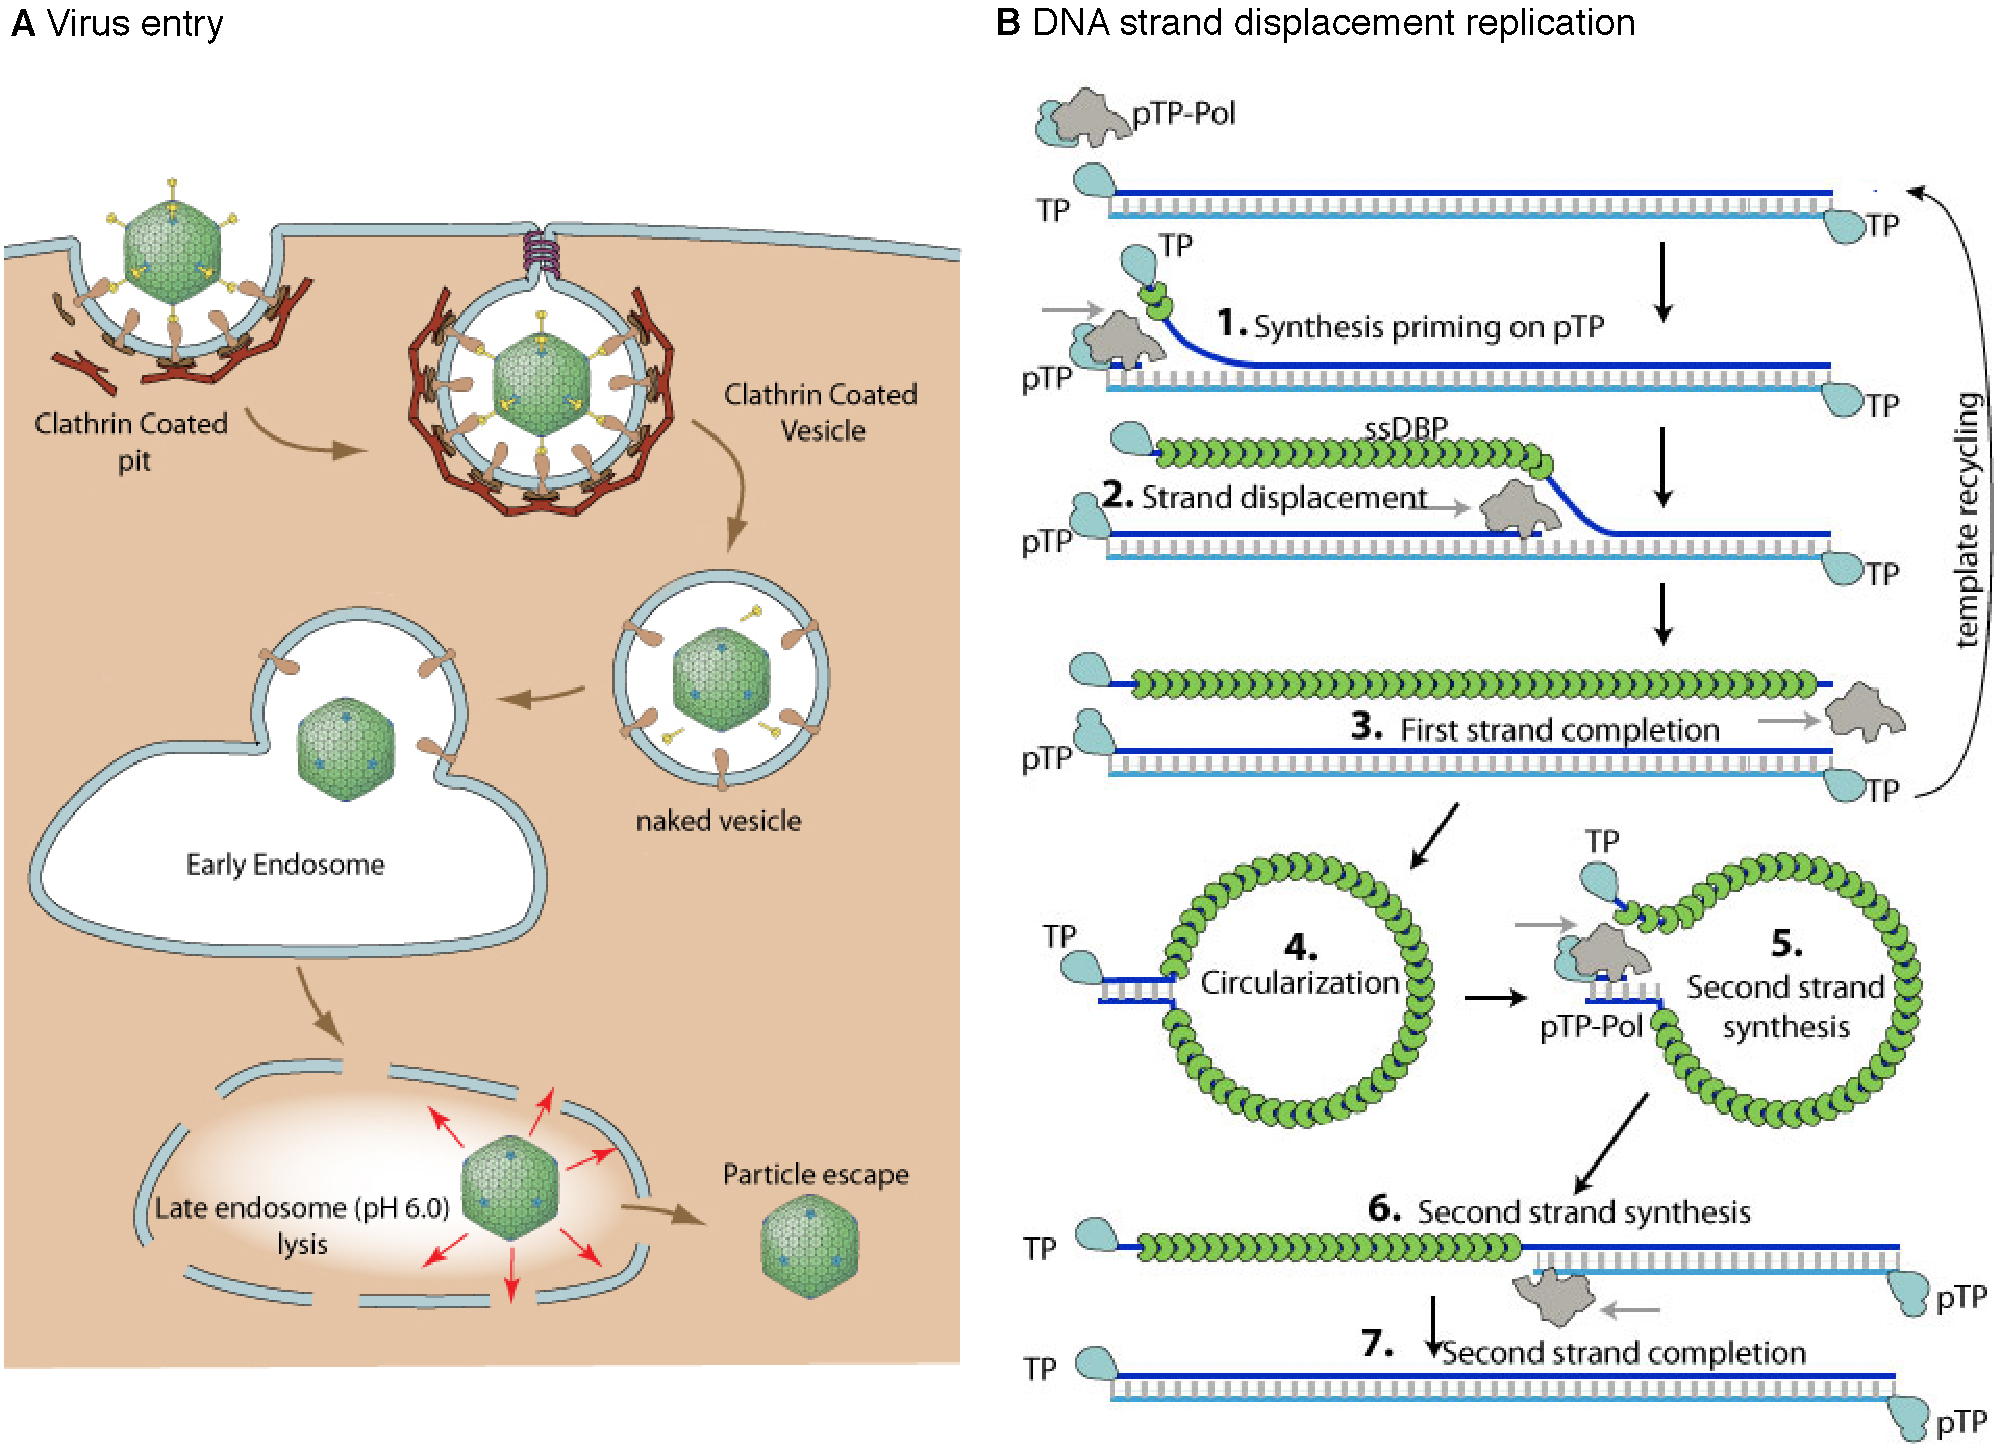
\includegraphics[width=0.95\textwidth]{adenovirus}
  \caption[Capsid structure and genome of rhinoviruses.]{Capsid proteins VP1 through VP4 form a pseudo $T=3$ icosahedral coat, roughly 30 nm in diameter around the RNA genome (A), which is monopartite, linear, 7.2 kp long and encodes 11 proteins (B). Figures adapted from \cite{Hulo2011}.}
  \label{fig:adenovirus}
\end{figure}

\paragraph{Pathogenesis.}
Initial attachment of virions is mediated by interactions between the globular knobs of viral fiber proteins and target cell \glsrevpl{car}. In \textit{Human adenovirus C} infections, cellular heparan sulfate proteoglycans serve as additional attachment factors, reinforcing adhesion. Subsequent binding of penton bases to \textalpha,\textbeta-integrin receptors induces clathrin-mediated endocytosis and leads to loss of viral fiber proteins.

The adenoviral replication cycle is divided into early, intermediate and late stages, with each seeing expression of a typical set of genes. Upon engulfment by the host cell and triggered by endosomal acidification, hexon bound protein VI disassociates from the capsid structure and induces lysis of the endosomal membrane. The remainder of the now cytosolic virion is shuttled to the nucleus by microtubular transport where viral protein IX recruits kinesin thereby procuring capsid disruption. Nuclear penetration is mediated by core protein VII and occurs at \glspl{npc}, leading to transcription of early viral genes by host RNA polymerase II. The resulting proteins manipulate various cellular processes, such as evasion of host immune response (E3), cell cycle (E1A), apoptosis (E1B and E4) and \gls{mrna} transport (E4), while also promoting viral DNA replication (E2). A virally encoded DNA polymerase replicates the genome by DNA strand displacement in a unique protein primed fashion involving \gls{ptp} acting as primer and \gls{dbp}, as well as several host proteins. With onset of replication, translation of late genes by host RNA polymerase II is initiated, leading to the production of structural proteins and proteins required for virion assembly. Encapsidation occurs in the nucleus and progeny virions are released by lysis of the host cell.

\paragraph{Epidemiology.}
Adenoviruses are endemic and ubiquitous, causing an estimated 2--5\%of all respiratory infections. Distribution is worldwide and incidence higher in the first half of the year. Children are frequently infected as serological studies show that by the age of 5 years some 50\% present antibodies towards the most common species, including \textit{Human adenovirus C}. On the order of 1 in every $10^7$ lymphoid cells in the oropharynx harbor fully assembled latent sate virions, making most humans latent carriers. Transmission can both occur via respiratory droplet or fecal-oral routes and virions are very stable towards chemical and physical agents, surviving for long periods outside their host.

Adenovirus outbreaks are a common cause of pneumonia in militaries, leading to the development of live, oral vaccines in the 1960's by the U.S. Army. The only supplier however ceased production and as of 1999, vaccinations could no longer be administered, resulting in reemerging incidence. In the first 5 years after loss of the vaccine, 110000 cases of febrile respiratory illness were reported, of which an estimated 90\% are considered preventable. By October 2011, new vaccine again was available and and has been administered to new recruits since.

\subsection{Rhinoviruses}
Investigations into the etiological agent of the common cold within the British Common Cold Research Unit led to the discovery of rhinoviruses in 1953. Initially classified as a separate genus of the family \textit{Picornaviridae}, recent genomic evidence led to a revised taxonomy, recognizing three species of rhinoviruses (A through C) as members of the genus \textit{Enterovirus}. Over 100 distinct serotypes have been isolated from humans, 74 belong to species A, 25 to B and the newly identified species C, currently under active study, may encompass an additional 55 types.

Rhinovirus virions are small (30 nm in diameter), non-enveloped, with a pseudo $T=3$ icosahedral capsid, consisting of 4 different polypeptides (VP1, VP2, VP3 and VP4) surrounding the RNA genome. There are 60 copies of each structural protein and VP1-3 face towards the outside and are responsible for antigenic diversity, while VP4 faces inwards and anchors the RNA core to the capsid. A canyon formed by VP1 and VP3 serves as receptor binding site. The viral genome consists of monopartite, linear, single stranded, positive sense RNA, roughly 7.2 kb in length and encodes a single polyprotein, which cleaved by viral proteases yields 11 proteins. Instead of a methylated 5' cap, the RNA genome is terminated by a viral protein (VPg) at its 5' end \citep{Jacobs2013}.

\paragraph{Diseases.}
Over half and up to two thirds of all cold-like illnesses are thought to be caused by rhinoviruses. In addition, asymptomatic infections, especially in children are very common with rates among children under 4 years ranging from 12 to 32\%. These surprisingly high numbers may to some extent result from virus persistence in hosts that have recovered in addition to disease that has not broken out. In adults, rates of asymptomatic carriage are significantly lower, reported at 0--2\%.

In immunocompetent individuals, symptomatic disease typically manifests as upper respiratory infection with clinical syndromes associated with common cold, including rhinorrhea, nasal congestion, sore throat, headache and possibly fever and general malaise. Disease is self-limited, incubation periods are between 12 and 72 h and within 7 to 14 days, symptoms wear off. A common complication is acute otitis media, which has been reported to happen in up to 30\% of cases in early childhood. In 41--45\% of investigated middle ear infections, rhinoviruses were detected. Further cavities that are frequently infected are the paranasal sinuses. Nose blowing has been suggested as mechanism for spreading the virus and causing rhinosinusitis.

Initially thought to primarily cause benign upper respiratory infections,  recent data clearly implicates rhinoviruses in more severe lower respiratory infections. Croup, bronchiolitis and \gls{cap} have been associated with rhinovirus infections and studies have shown that in 12, 14 and 18--26\% of respective cases, rhinoviruses were present. Furthermore, a study of children admitted to \glspl{icu} with lower respiratory tract infections detected no other pathogens in 49\% of the patients. Immunocompromised individuals are predisposed to contracting more serious forms of disease, with morbidity and mortality comparable to that of pandemic H1N1 influenza.

While not typically associated with cytopathogenic effects on epithelia of the upper respiratory tract, cell damage to lung tissue, especially among children, has been documented. Thus, rhinoviruses are linked to exacerbations of chronic pulmonary diseases such as asthma, chronic obstructive pulmonary disease and cystic fibrosis.

\begin{figure}
  \centering
  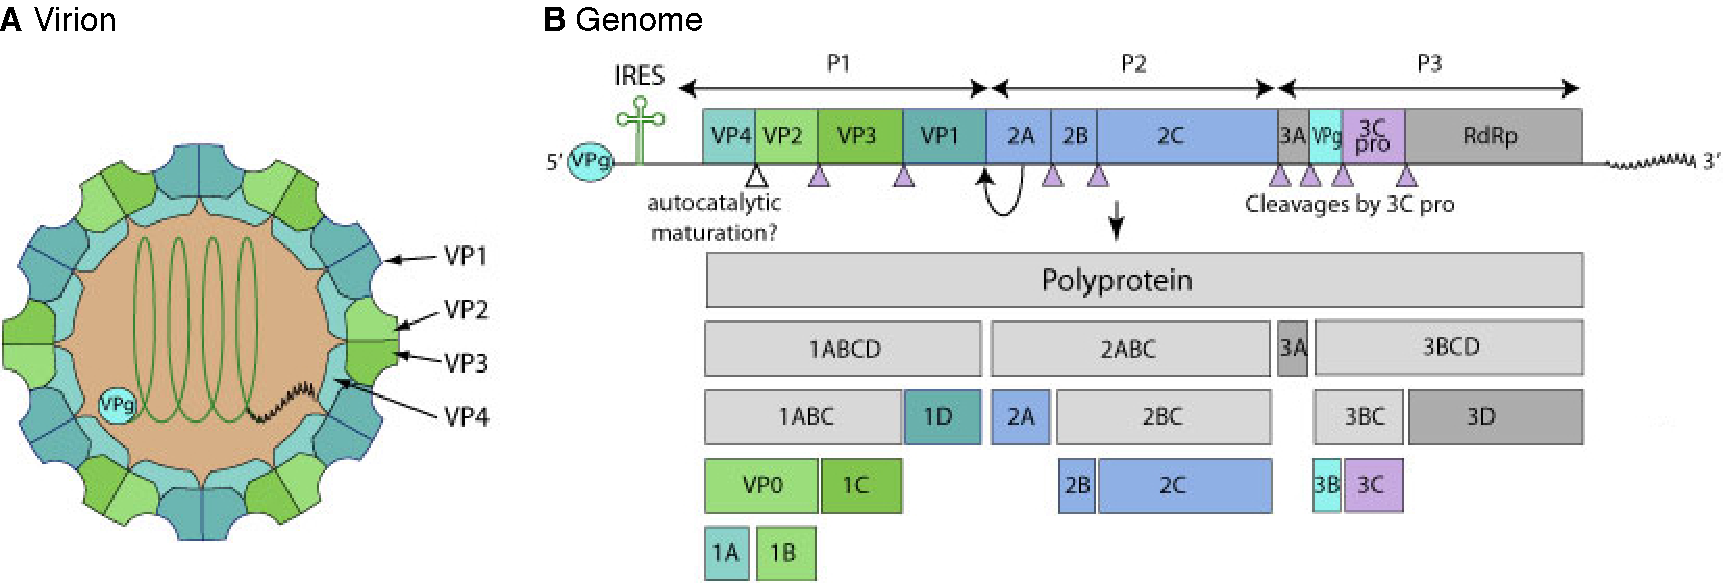
\includegraphics[width=0.95\textwidth]{rhinovirus}
  \caption[Capsid structure and genome of rhinoviruses.]{Capsid proteins VP1 through VP4 form a pseudo $T=3$ icosahedral coat, roughly 30 nm in diameter around the RNA genome (A), which is monopartite, linear, 7.2 kp long and encodes 11 proteins (B). Figures adapted from \cite{Hulo2011}.}
  \label{fig:rhinovirus}
\end{figure}

\paragraph{Pathogenesis.}
Members of rhinovirus species A and B are divided into two group according to their host cell receptors. Members of the major group form interactions with \gls{icam-1} while minor group types (including serotype 1a) associate with \glspl{vldlr}. Attachment of species C have very recently been identified as induced by \gls{cdhr3}. Upon receptor mediated endocytosis, pH dependent conformational changes in capsid structure exposes VP4 which has pore-forming properties and facilitates release of viral genomic material into the cytosol.

Host cell ribosomes readily translate the released positive-sense RNA into polyprotein, which is cleaved in \textit{cis} by 2A and 3Cpro, yielding preproteins P1, P2 and P3 (see figure \ref{fig:rhinovirus}. P1 is digested into structural capsid proteins while P2 and P3 are further processed to produce the replication machinery. Viral RNA-dependent RNA polymerase synthesizes a complementary, negative-sense RNA strand, primed by VPg, which in turn serves as template for many copies of the viral genome. These can be both translated into more protein and in a later stage of replication also be packaged into progeny virions. Final cell export is mediated by host-cell membrane lysis.

\paragraph{Epidemiology.}
Despite most infections with rhinoviruses only resulting in mild disease, economic impact both due to health care costs and loss of productivity is considerable. This is primarily owed to the overwhelming prevalence of these pathogens. Respiratory illnesses attributed to rhinoviral infections occur throughout the world and all year round with peak incidences in early fall and spring. Vaccination efforts so far have been futile, mainly because of the large number of serotypes and lack of individual epidemiological data.

Due to acid-sensitivity, fecal-oral infection is unlikely most person-to-person transmission occurs through aerosols and contact spread either direct of via fomites. Extra-host survival times of hours to days have been reported for indoor environments and up to 2 h on undisturbed skin.

\subsection{Vaccinia}
\textit{Vaccinia virus} is a species within the genus \textit{Orthopoxvirus}, alongside the exceptionally virulent \textit{Variola virus}, the etiological agent of smallpox. Immunological similarities between the two species allows for cross-protection, which coupled with the large discrepancy in pathogenicity presents a fortunate opportunity for artificially inducing acquired immunity. This was recognized by Jenner in 1798, while investigating the zoonosis of \textit{Cowpox virus} and subsequent susceptibility towards contraction of smallpox. The origins of vaccinia are unknown. It has been speculated to have derived from cowpox or smallpox, to be a hybrid of both and of being the prototype orthopoxvirus, as well as descending from an extinct ancestor.

The virions are large and brick shaped, measuring 200 by 250 by 340 nm and exist as both \gls{mv} and \gls{ev}. Structurally they are unusually complex. The linear, double-stranded DNA genome, roughly 200 kb long, is encased in an S-shaped, tube-like nucleocapsid with an outside diameter of 50 nm, a cavity of 10 nm and an overall length of 250 nm. Additionally, 47 viral proteins, of which 16 are involved in early \gls{mrna} synthesis and 28 have no known enzymatic function, are packed into a core structure. The core wall consists of two layers, the palisade (outer) layer which is 17 nm thick and an inner smooth layer, measuring 8 nm across. Centered on the top and bottom faces, two proteinaceous lateral bodies separate core from the surface membrane, forming the virion core into a biconcave disc with dumbbell shaped vertical cross sections. The lipidic surface membrane also consist of two layers, the outermost measuring 9 nm and the innermost domain is 5 nm thick. \Gls{ev} virions are additionally wrapped in a membrane derived from Golgi cisternae \citep{Marennikova2005,Condit2006}.

\paragraph{Diseases.}
While infection with variola causes severe disease manifesting in skin lesions covering the whole body, accompanied by 20--40\% mortality rates, the closely related \textit{Vaccinia virus} is far less invasive. Virulence of the latter pathogen is so low that it has been routinely used as live vaccine against the former. Owing to the massive effort put into the worldwide fight against smallpox led by the \gls{who} in the late 1960's and throughout the 1970's, the disease was found to be eliminated by 1980. At the center of the smallpox eradication program was the administration of freeze-dried, calf lymph derived vaccinia with a bifurcated needle, by multiple pricking of the skin. Towards the end of the initiative, 200 million vaccinations were performed annually.

The predominant reaction to vaccinia inoculation is localized, self-limited disease. After an incubation period of of 3--4 days, a papule with a sunken center develops at the site of infection, accompanied by erythema and swelling. Over the following days the papule increases in size and liquid begins to accumulate within. Fever may develop around days 7--10, possibly followed by malaise, headache and anorexia. Local lymphadenopathy is frequently encountered and days 8--10 typically mark the beginning of involution of the papule, which subsequently drys out and forms a scab.

Of great concern for routine vaccination procedures are complications which inevitably occur in a small numbers. Atypical side effects develop in roughly 1 per mill of cases and potentially life threatening reactions usually manifest as neurological (477.4 cases and 47.0 fatalities per 1 million) or cutaneous disease (278.4 cases and 0.2 fatalities per 1 million). Predisposing conditions for central nervous system involvement are not known and despite decades of inquiry into this pathology, it remains poorly understood. Symptoms range from febrile seizures to severe encephalitis, but so far no  neuropathological characteristics have been identified. Complications affecting the skin and mucous membranes are classified as progressive vaccinia, eczema vaccinatum and generalized vaccinia and disease severity decreases in this order. Predisposing conditions for progressive and generalized vaccinia are immunodeficiencies while a history of eczema is a risk factor for eczema vaccinatum.

\begin{figure}[t]
  \centering
  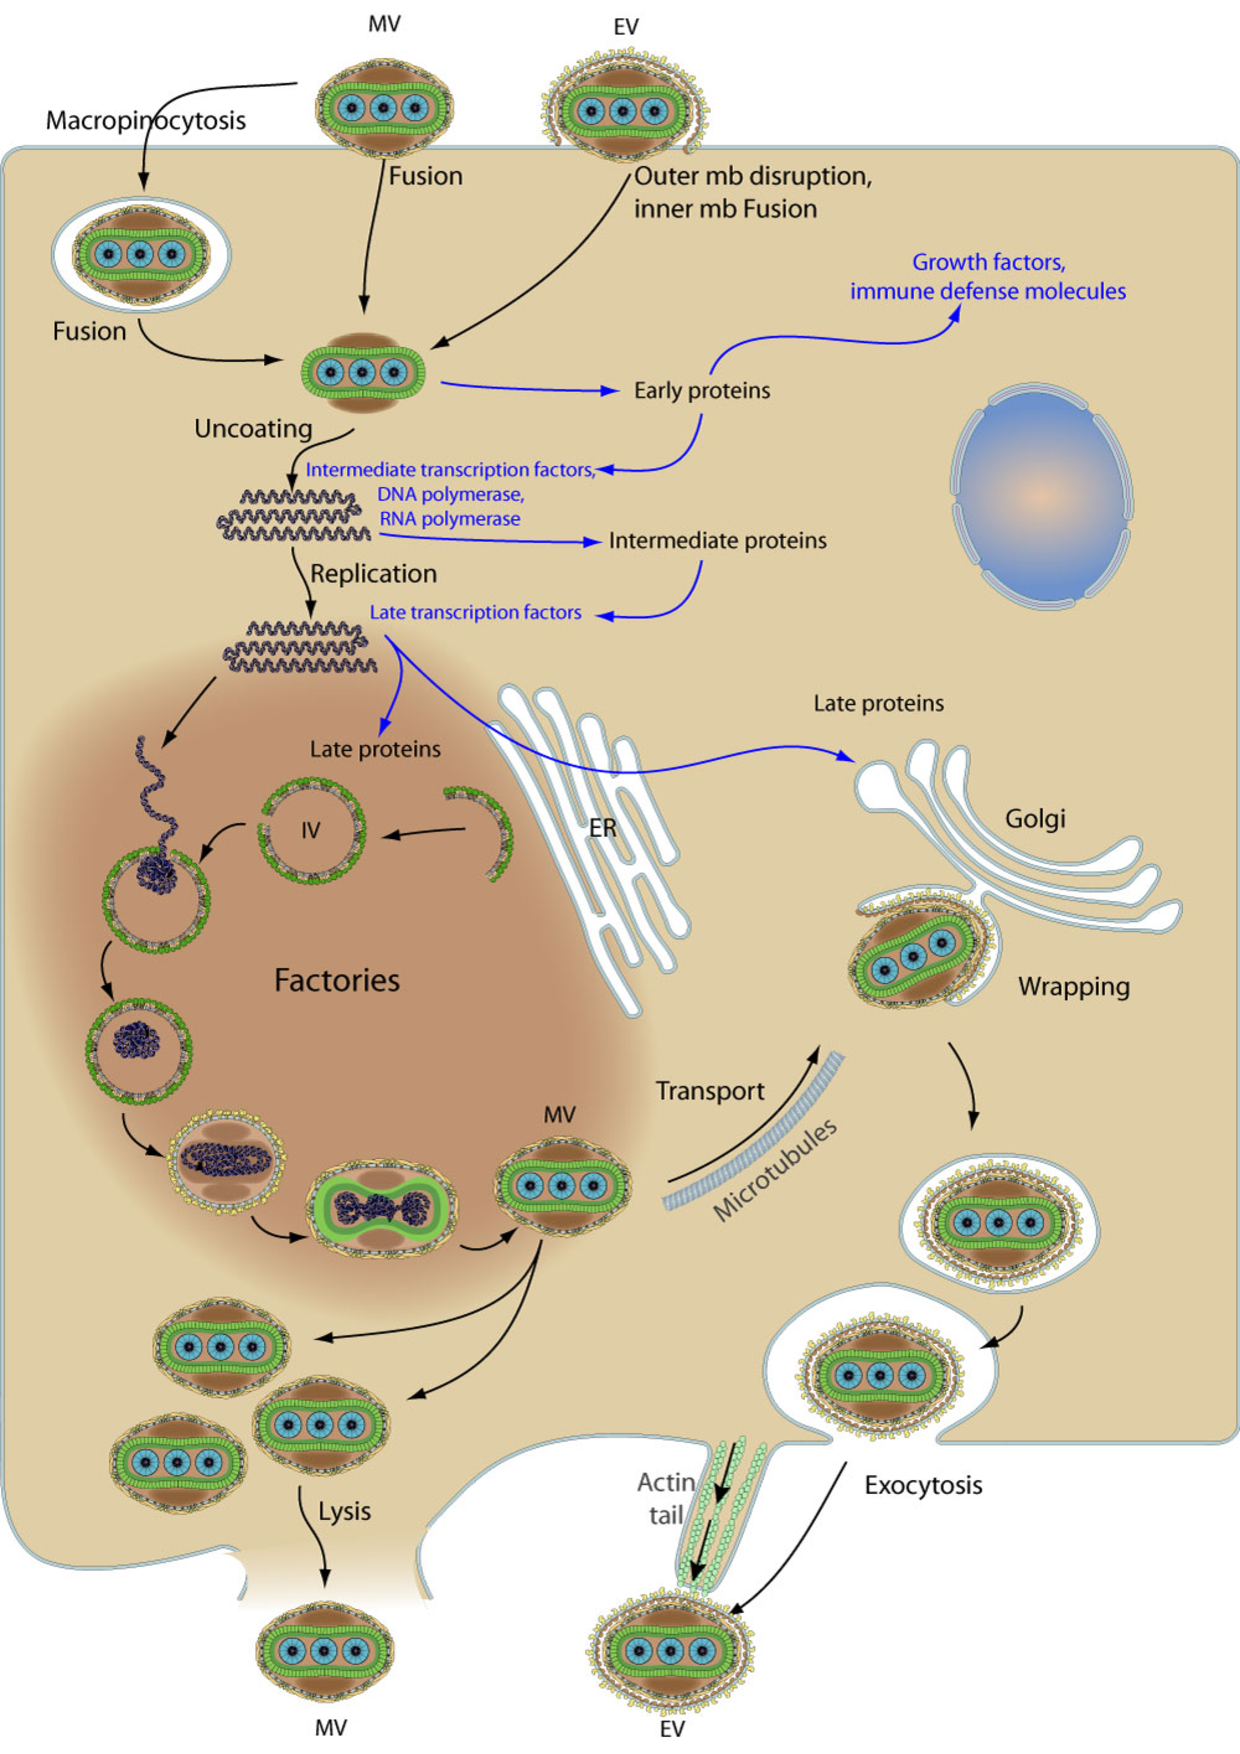
\includegraphics[width=0.75\textwidth]{vaccinia}
  \caption[Replication cycle of \textit{Vaccinia viruses} for both intracellular mature and extracellular enveloped virions.]{Capsid proteins VP1 through VP4 form a pseudo $T=3$ icosahedral coat, roughly 30 nm in diameter around the RNA genome (A), which is monopartite, linear, 7.2 kp long and encodes 11 proteins \citep{Hulo2011}.}
  \label{fig:vaccinia}
\end{figure}

\paragraph{Pathogenesis.}
Initial attachement is mediated by interaction between viral proteins and cellular heparan sulfate chains. For cell entry, various strategies have been reported, depending on the strain under investigation. WR strains induce macropinocytosis and proteins A25/A26 act as fusion suppressors that only lift their embargo under acidic conditions encountered in a maturing endosome, while other strains, such as Copenhagen, present no A25/A26 on their outer membrane and fuse directly with the target plasma membrane. Due to the additional membrane of \glspl{ev}, a differing entry mechanism needs to be emplyed. In a currently not well understood fashion, the outer membrane is lost by non-fusogenic disruption, followed by fusion of the inner virion membrane. All pathways lead to cytosolic localization of virions devoid of their envelope.

Members of the \textit{Poxviridae} family are special among Baltimore group I viruses in that their genome encodes all necessary replicatory proteins, allowing for cytosolic localization. Replication is temporally tightly regulated and consist of distinct phases of early, intermediate and late gene expression. Each class of genes encodes factors capable of initiating the succeeding stage, providing transcription level regulation. Uncoating of the core structure releases early proteins, including RNA polymerases and enzymes for \gls{mrna} processing which start transcribing early genes. At least 50 different products, such as DNA replicatory enzymes, additional RNA polymerase, \gls{mrna} processing machinery, host defense molecules and intermediate gene transcription factors, have been identified and account for 25\% of the viral coding capacity. Early gene transcripts are detectable 20 minutes after cell entry and reach their productive peak within 100 minutes of infection.

Expression of intermediate genes is initiated by accumulation of intermediate  transcription factors and the onset of DNA replication. Only 7 products of this phase are known, which functionally are mostly concerned with host defense, DNA/RNA metabolism and commencement of the final phase. Beginning 100 minutes after infection, intermediate gene transcription reaches its peak at 120 minutes and is thereafter superseded by late gene transcription, beginning 140 minutes after cell entry. Products of the final phase comprise a large number of genes (up to 75\% of the vaccinia genome) and include enzymes needed for initiating replication (RNA polymerase and modification proteins), early transcription factors and structural proteins, as well as virion assembly machinery.

DNA replication not only serves for progeny virions, but also to increase the concentration of templates used for gene expression. Both DNA synthesis and virion assembly occur within factories, readily visualized by electron microscopy as electron dense cytoplasmic inclusion bodies. Owing to the complex virion structure DNA packaging and virion assembly is an involved procedure with is incompletely understood.

\paragraph{Epidemiology.}
It is unknown if a natural reservoir of vaccinia exists It has been speculated that the virus is maintained only within research laboratories and vaccination production facilities, while others have implicated some rodent species as possible reservoir hosts. Small scale zoonotic outbreaks of vaccinia have been documented in Brazil and it was initially suspected that these were linked to vaccine that had escaped into the environment. Recent phylogenetic studies however were able to rule out this explanation but were unable to shed further light into underlying epidemiological mechanisms.

While transmission from vaccinees to unvaccinated individuals is rare, direct contact transmission is possible and such occurrences have been documented. Special care has to be taken to avoid direct contact between recently vaccinated and individuals predisposed towards developing complications.

\section{RNA Interference}
First described only two decades ago, regulation of gene expression by short strands of RNA has become an indispensable tool to both experimental biology and bioinformatics. Recognizing the importance of applications made possible by this discovery, the 2006 Nobel prize in Physiology or Medicine was awarded to Fire and Mello who studied RNA interference in the nematode worm \textit{Caenorhabditis elegans} and published their findings in 1998. Building on studies by Guo and Kemphues, who showed that sense RNA, as well as antisense RNA was capable of suppressing gene expression, Fire, Mello and coworkers found that double stranded RNA was at least ten-fold more effective as silencing agent than individual single stranded fragments. Further investigations showed that several gene regulatory processes, previously thought to be unrelated, were in fact manifestations of RNA interference and that the underlying mechanism was conserved in many if not most eukaryotic organisms \citep{Hannon2002}.

The RNAi pathway can take as input two separate types of RNA molecules, \gls{mirna} and \gls{sirna}, of differing origins. While \glspl{mirna} are endogenous and purposively employed in post-transcriptional regulation of gene expression, \glspl{sirna} are exogenous synthetic or viral inducers of gene suppression, in which case, RNA interference can be viewed as an immune response to foreign genetic material. Parsimony-based phylogenetic analysis of involved genes suggests that the key components to an RNAi system were already present in the last common ancestor of eukaryotes and were subsequently lost or extensivley simplified in some protists. The original function of RNAi is hypothesized to be that of a defense mechanism against genomic parasites as indicated by the extent of its conservation, whereas \gls{mirna}-directed silencing most probably was introduced at a later point in evolution \citep{Cerutti2006}.

\subsection{Molecular Mechanism}
RNA interference refers to three separate mechanisms for regulation of gene expression by small RNAs, as visualized by figure \ref{fig:rnai}. While \glspl{sirna} are involved both in transcriptional and post-transcriptional gene silencing, the \gls{mirna} pathway is focused on translational repression. The severity of action on the targeted genes once again highlights the differing purposes of the \gls{sirna} and \gls{mirna} pathways, one tasked with inhibitory and the other with regulatory measures \citep{Wilson2013,Kim2007,Carthew2009}.

\begin{figure}[t]
  \centering
  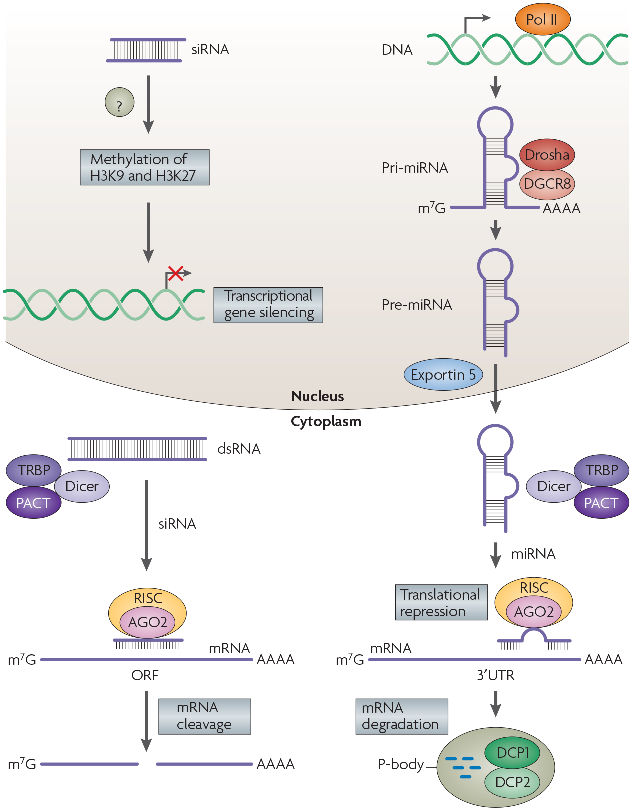
\includegraphics[width=0.7\textwidth]{rnai}
  \caption[The three major pathways of RNA interference.]{RNA interference comprises of three distinct mechanisms that yield control over gene expression. Exogenous double-stranded RNA are processed into \gls{sirna} fragments that both act inside the nucleus as transcriptional silencing agents and in the cytoplasm, post-transcriptionally cleaving \gls{mrna} strands. Endogenous \gls{mirna} is synthesized by RNA polymerase, originates from the nucleus in processed form and mediates milder translational repression \citep{Kim2007}.}
  \label{fig:rnai}
\end{figure}

\paragraph{Translational repression by \gls{mirna}.}
The biogenesis of \gls{mirna} occurs in the nucleus and is initiated by RNA polymerase II transcription of long (\textgreater 1000 nt) \gls{pri-mirna} segments, characterized by double-stranded hairpin loops with single-stranded 5'- and 3'-terminal overhangs which are polyadenylated and capped. Subsequent processing by the microprocessor complex consisting of the RNase III family enzyme Drosha and \glsrev{dgcr8} yields \tilde 60--70 nt stem-loop structured \gls{pre-mirna} fragments. \gls{dgcr8} recognizes \glspl{pri-mirna} by the junction of stem and single-stranded overhang and helps positioning the substrate for endonucleolytic cleavage by Drosha at a site \tilde 11 nt from the junction. Nuclear export is mediated by the transport facilitator exportin-5 and is Ran-GTP dependent.

In the cytoplasm, \glspl{pri-mirna} are targeted by Dicer and the associated dsRNA binding proteins \glsrev{trbp} and \glsrev{pact} for further processing into 21--25 nt dsRNA strands with 2 nt overhangs at the 3' termini and phosphate groups at each of the recessed 5' ends. The mature \glspl{mirna} are loaded onto \gls{ago} by Dicer, which leads to the formation of \gls{risc}. Concomitantly with \gls{risc}-loading, one of the two RNA stands is selected as guide strand whereas its complement (the passenger strand) is ejected and degraded. Thermodynamic asymmetry between the two strands is exploited in this step and the strand with the less stable 5' end is preferred. As opposed to strand separation in \glspl{sirna}, the passenger strand is not cleaved but rather unwound by helicase activity, facilitated by imperfect sequence alignment.

Finally, active \gls{risc}, exposing the \glsdesc{ago}-bound guide strand, interacts with the 3' untranslated region of \gls{mrna} targets and directs translational repression and \gls{mrna} degradation. Sequence homology between \gls{mrna} and the \gls{mirna} seed sequence (the first 2--6 or 2--8 nt from the 5' end) is critical while mismatched nucleotides towards the 3' end of the \gls{mirna} are readily tolerated. The extent of base-pairing influences the subsequent mechanism of silencing, ranging from direct target cleavage (perfect match) over deadenylation (followed by degradation), to nonendonucleolytic translational repression (imperfect match).

\paragraph{Post-transcriptional gene silencing by \gls{sirna}.}
Precursors to \gls{sirna} are long, linear, perfectly base-paired double stranded sequences of RNA, typically of exogenous origin either introduced directly into the cytoplasm, or taken up from the environment. A complex consisting of Dicer and several RNA-binding proteins are responsible for trimming down dsRNA fragments to the appropriate size for loading onto \gls{ago}2. Of the four \glsdesc{ago} family members in humans, capable of associating with \gls{mirna}, only \gls{ago}2 seems to be involved with \gls{sirna}. Furthermore, \gls{ago}2 is the only mammalian \glsdesc{ago} bearing endonucleolytic functionality and therefore capable of directly cleaving targeted \gls{mrna}.

Strand selection is again based on differences in stability of base-pairing at the 5' termini with the weaker interacting end being favored as guide strand. Accuracy of discrimination can be low, leading to incorporation of both strands with equal frequency. In contrast to \gls{mirna} loading, the passenger strand is not merely separated but directly cleaved by \gls{ago}2 and the differing treatment seems to only depend on perfect strand complementarity given in \gls{sirna} and absent in \gls{mirna}. Upon RNA incorporation, \gls{risc} is formed and activated by cleavage of the passenger strand. The 3' guide strand end is bound by the \glsdesc{ago}'s \gls{paz}, while the 5' end interacts with \gls{mid}, closely located to the catalytic RNase H-like \gls{piwi}.

Post-transcriptional gene silencing is accomplished by endonucleolysis of perfectly matching \gls{mrna} precisely at the phosphodiester linkage between bases 10 and 11 relative to the 5' terminus of the \gls{sirna} guide strand. Following cleavage, the target disociates, freeing \gls{risc} for further catalysis, and the \gls{mrna} fragments are degraded by cellular exonucleases. Imperfectly matched \gls{mrna} may be targeted, much like it is the case with \gls{mirna}, leading to \gls{sirna} off-target effects which are of great practical importance.

\paragraph{Transcriptional gene silencing by \gls{sirna}.}
In addition to post transcriptional action of \gls{sirna}, nuclear inhibition of gene transcription has been described in many eukaryotes. Diced \gls{sirna} fragments are transported into the nucleus where they are assembled with a group of proteins, including \gls{ago}1, to form \gls{rits}. Currently only incompletely understood, the \gls{sirna} guide strand is thought to recognize RNA transcripts as the emerge from RNA polymerase II, followed by recruitment of factors that enable covalent modifications of nearby histones. Methylation of lysines 9 and 27 in H3 by histone methyltransferases leads to chromatin compaction and heterochromatin formation. \Gls{rits} has also been shown to induce direct methylation of DNA, repressing gene expression even further.

Contributing to the potency of RNA interference, engagement of \gls{rits} with nascent transcripts activates the \gls{rdrc}, capable of generating secondary \gls{sirna} fragments and therefore amplifying silencing capabilities. The role of this reinforcement mechanism has been firmly established in many eukaryotic RNAi systems with the notable exceptions of vertebrates and insects. Whether a similar system exists in these organisms remains an open question.

\subsection{Biological Function}
The mechanisms of RNA interference have most probably evolved in order to protect against foreign genetic material such as parasitic DNA sequences or viral RNA. Transposable elements (transposons) are DNA sequences that are mobile within the genome, can make up a significant fraction of eukaryotic genomes and are typically considered non-coding. Transposition is mediated by transposases, enzymes often encoded within the transposons themselves, that act on specific sequences at the transposon ends and cause unspecific insertion into new target sites. Retrotransposons move via an RNA intermediate which is reverse transcribed to DNA and inserted, while DNA transposons employ a cut and paste mechanism. Retroviruses therefore can be viewed as transposons and in general, transposable elements are a form of selfish DNA that often incur deleterious effects.

RNAi is an important regulatory force to transposon activity, both by processing transcripts of retrotransposons, thereby reducing their concentration and eliciting epigenetic modifications, as well as transcriptional inhibition via heterochromatin formation. The importance of keeping transposable elements in check is highlighted by their prevalence, with roughly half of the human genome being thought to derive thereof.

Antiviral mechanisms are particularly important in organisms lacking an adaptive immune system as found in vertebrates and exploiting the orthogonality of most genomic systems to double-stranded RNA puts RNA interference in a powerful position. Corroborating this notion is the observation that, in \textit{Drosophila melanogaster}, three key proteins of the RNAi pathway (Dicer-2, \gls{ago}2 and R2D2, a protein involved in \gls{risc} loading) are among the top 3\% in terms of genetic instability. Furthermore, \gls{mirna} pathway paralogs to these three genes (Dicer-1, \gls{ago}1 and R3D1), not being involved in immune response, evolve at a much slower rate \citep{Obbard2009}.

Although small RNA-guided, \gls{ago}-dependent up-regulation of gene expression (termed RNA activation or RNAa) has been described, most regulation of gene expression by \gls{mirna} is of inhibitory nature. This widespread mechanism, consisting of \textgreater 1000 \gls{mirna} sequences (as much as 5\% of the human genome) controls at least 30\% of human genes and is responsible for vital processes including cell growth, tissue differentiation and cell proliferation.

\subsection{Applications}
In \textit{C. elegans}, RNA interference is especially powerful, making it a popular model organism for RNAi. Not only is delivery efficiently possible simply by feeding the nematodes with bacteria such as \textit{E. coli} that carry the desired dsRNA, but the resulting gene silencing effects are hereditary. Moreover, RNAi response is not stoichiometric but catalytic, is amplified in a feedback loop and in many organisms, systemic spread has been documented.

The initial burst of excitement surrounding possible applications was somewhat moderated by difficulties in applying RNAi to mammalian systems. At first it seemed impossible to use this technology in somatic cells as the introduction of dsRNA is typically met with overwhelming non-specific responses, including  \gls{pkr}, which leads to arrest of translation and apoptosis. This issue was shown to be overcome by exclusively using \glspl{sirna} duplexes of 21--23 nt with 2-nt 3' overhangs that mimic Dicer products and are too short for inducing \gls{pkr}. Mammalian RNAi response, however is transient, lacking amplification and spreading mechanisms documented in other organisms (mainly plants and worms) and delivery, especially in vivo remains problematic. A further issue that continues to be an actively researched area of interest is that of \gls{ote}, which considerably complicate the interpretation of phenotypic data.

\paragraph{Gene knockdown studies.}
Large-scale \gls{lof} and modifier or synthetic lethality screens are readily possible by means of RNAi based \gls{hts}. Such experiments usually proceed by arraying libraries of gene specific \glspl{sirna} onto microtiter plates (96 and 384 well formats are common), followed by the addition of liquid cell cultures. After an appropriate transfection time, the cells may be subjected to an additional treatment, such as exposure to drugs or pathogens (modifier screen) or \gls{lof} phenotypes can be investigated directly. Assay readout is performed via optical measurements such as detection of fluorescence or luminescence signals or by microscopic imaging (confocal or wide-field).

Transcriptional reporters, fluorescent dyes that detect enzymatic activity and protein-modification specific antibodies have been employed in plate reader-based investigations which yield a single numerical readout per well. This quantitative approach is contrasted with microscopy based assay read-outs that are able to capture spatial information on antibody stained proteins, fluorescently labeled cellular structures and \gls{gfp} expression, yielding much more data per well. Significant challenges incurred by automated high-content imaging have successfully been addressed by computational image analysis software.

A multitude of sources of technical and biological noise contribute to serious problems in interpretability and comparability of observed data. Common to all high throughput approaches, errors arise from difficulties guaranteeing equal conditions in a large number of parallel experiments. Liquid dispensing errors, temporal disparities caused by bottleneck resources such as imaging equipment and spatial discrepancies, for example inhomogeneous temperature distribution over the plate, are only a few issues that come to mind. Biological sources of error include \glspl{ote}, varying potency of reagents (both the knockdown strength and time required to achieve optimal knockdown may be affected) and obscuration of assay phenotype by the knockdown phenotype (e.g. cell death). Furthermore, incorrect gene models lead to errors in library design and detection may be hampered by weak phenotypes. Replicates, although expensive in large-scale experiments and control wells embedded in every assay plate are indispensable measures in order to assess reproducibility of the data \citep{Echeverri2006,Perrimon2007}.

Despite being a young technology, RNA interference has already proven itself as an invaluable tool and has yielded many insights with significant impact on various fields. A review by \cite{Mohr2010} lists some of these findings which lead to refined understanding of cell proliferations, cancer biology, cell cycle regulation, mitochondrial diseases, signal transduction, RNA biology and pathogen response. 

\paragraph{Biotechnological applications.}
Intercellular, systemic spread of RNAi response in plants and even its heredity over several generations have been documented and it comes as no surprise that the technology is investigated for possible utilization in crop improvement. Removal of plant endotoxins by targeting genes of toxin biosynthesis has been accomplished, leading to the production of decaffeinated coffee plants (knockdown of theobromine synthase), tobacco with reduced concentration of carcinogenic compounds (inhibition of nicotine demethylase activity) and edible cotton seeds (reduction of delta-cadinene synthase leads to low levels of gossypol, a toxic terpenoid), which are naturally rich in dietary protein.

In addition to investigations with consumer health in mind, improvements in environmental resistance have been studied in many organisms. Susceptibility to bacterial and viral pathogen infection has been reduced in rice, bean, barley and lemon, while fungal resistance has been increased in potato, tobacco and wheat. Successful RNAi application as insecticide has been shown in cotton and maize and even improved resistance to parasitic weeds could be demonstrated in transgenic tomato plants. Despite these achievements, concerns over environmental issues and adverse health effects have so far prevented RNAi based genetic modifications from exiting experimental stages \citep{Saurabh2014}.

\paragraph{Therapeutic potential.}
Great promise lies in therapeutic application of RNAi as theoretically, any gene can be targeted, yielding unparalleled flexibility not encountered with typical small molecule drugs. An initial obstacle to harnessing this power in humans is the issue of delivery. Systemic spread of naked \glspl{sirna} is hampered by kidney filtration, phagocytic uptake and degradation by serum RNases. Movement across capillary walls is not readily possible for molecules larger than 5 nm and phagocytes patrol the extracellular matrix, ingesting foreign genetic material. Furthermore, polyanionic macromolecules do not easily penetrate hydrophobic cellular membranes.

Topical or local administration offers advantages, including increased bioavailability and reduced side effects and is therefore preferred for treatment of eye, skin and mucosal diseases, as well as localized tumors. If targets are not localized or difficult to reach, injection into the bloodstream may provide a mode of systemic application. Chemical modification of the RNA backbone (2'-O-methylation or 2'-fluorination of ribose) has been shown to provide resistance to RNase and covalent attachment to cholesterol promotes cellular uptake. Encapsulation of \gls{sirna} in liposomes and cationic polymers are further proven techniques for improving extracellular stability, stimulate endocytosis and facilitate endosomal escape.

Some sort of target selectivity is desirable on order to avoid high dosages, associated concerns of toxicity and potential \glspl{ote} in non-target tissue. Coupling of \gls{sirna} reagents to antibodies specific for \gls{hiv} envelope glycoproteins has been successfully employed for selectively entering infected cells, while aptamers (oligonucleotides specifically engineered for binding a given target), carrying \glspl{sirna} have also been shown to be capable homing mechanisms.

Viral delivery of of RNAi inducing agents presents an alternative technique to the above and in case of retroviral transport vessels, \glspl{shrna} that are reverse transcribed and integrated into the host genome, provide stable expression and prolonged RNAi activity. Adenoviral and \gls{aav} vectors have also been employed, resulting in a more transient response. While health concerns associated with perpetuity of gene therapy no longer apply, repeated administrations may prove problematic, triggering strong immune response and thereby limiting therapeutic potential.

\begin{table}
  \centering
  \caption[A selection of RNAi based drugs in clinical trials.]{A non exhaustive list of RNAi based drugs that currently are in clinical trials. The data was obtained from \cite{McCray2000}}
  \label{tab:rnai-clinical}
  \footnotesize
  \begin{tabular}{L{1.5cm}L{3cm}L{2.5cm}L{2cm}}
    Company &
      Disease &
      Delivery system &
      Status \\
    \hline 
    Alnylam &
      (TTR)-Mediated Amyloidosis &
      siRNA–GalNAc conjugate &
      Phase III recruiting \\
    Alnylam &
      Antitrypsin Deficiency Liver Disease &
      Liposome &
      Phase II recruiting \\
    Alnylam &
      Acute Intermittent Porphyria &
      siRNA–GalNAc conjugate &
      Phase I recruiting \\
    Silenseed &
      Advanced pancreatic cancer &
      Polymer (LODER) &
      Phase III planned \\
    Sylentis &
      Ocular pain &
      Naked \gls{sirna} &
      Phase II completed \\
    Sylentis &
      Open angle glaucoma &
      Naked \gls{sirna} &
      Phase II recruiting \\
    Tacere &
      Chronic hepatitis C &
      \gls{aav} vector &
      Phase II recruiting \\
    Tekmira  &
      Cancers &
      liposome &
      Phase I active
  \end{tabular}
\end{table}

Currently, multiple \gls{sirna} based therapeutics are in clinical trials, including stage III studies (see table \ref{tab:rnai-clinical}). Due to the unprecedented pace at which RNAi technology went from discovery to development of applications, much uncertainty remains surrounding long term effects of exposure to such drugs. Chronic diseases including hepatitis C or \gls{hiv} infections require life-long treatments and consequences of repetitively triggering RNAi response has not been thoroughly studied (unwanted changes to chromatin structure for example, are one area of concern). Apart from safety issues, several implementation aspects require further study. While neurodegenerative diseases have successfully been treated in mouse models via direct injection into the brain, this is not easily feasible in human patients and currently no delivery vehicle capable of crossing the blood-brain barrier. \citep{Kim2007,Whitehead2009},

\chapter{Mathematical Background}

Modeling the relationship among variables is one of the most important applications of statistical theory. The study of regression analysis (and the closely related notion of correlation) started to form towards the end of the 19th century with Sir Francis Galton's study of height heredity in humans and his observation of regression towards the mean. Over the next few years, Udny Yule and Karl Pearson cast the developed concepts into precise mathematical formulation, in turn building on work performed by Adrien-Marie Legendre and Carl Friedrich Gauss who developed the method of least squares almost a century earlier \citep{Allen1997}.

A multiple linear regression model can be written in matrix-vector form as
\begin{equation}
  y = X \beta + \epsilon
\end{equation}
where $y \in \R^n$ is the vector of observations on the dependent variable, the design matrix $X \in \R^{n \times p}$ contains data on the independent variables, $\beta \in \R^p$ is the $p$-dimensional parameter vector and the error term $\epsilon \in \R^n$ captures effects not modeled by the regressors. Without loss of generality, all variables are assumed to be expressed as deviations from their means and measured on the same scale.

In order to find unknown coefficients $\beta_i$, the ordinary least squares estimator minimizes the residual sum of squares, the squared differences between observed responses and their predictions according to the linear model.
\begin{subequations}
\begin{align}
  \Hbeta &= \argmin_{\beta} \norm{y - X \beta}^2 \\
         &= (X^T X)^{-1} X^T y \label{eq:olsEstimate}
\end{align}
\end{subequations}
Some assumptions are typically associated with linear regression models that yield desirable attributes for the estimates. None of these restrictions are imposed on the explanatory variables; they can be continuous or discrete and combined as well as transformed arbitrarily. Furthermore, in practice, it is irrelevant whether the covariates are treated as random variables or as deterministic constants. With exception of the field of econometrics it appears that the majority of literature adheres to the latter interpretation and therefore, statements will not explicitly be conditional on covariate values.
\begin{description}
  \item[Linearity.] The relationship between dependent and independent variables should be linear (after suitable transformations) and individual effects additive. If this cannot be satisfied, a linear model is not suitable.
  \item[Full rank.] For the matrix $X^T X$ to be invertible, it has to have full rank $p$. Therefore $n \leq p$ and all covariates must be linearly independent.
  \item[Exogeneity.] All independent variables should be known exactly i.e. contain no measurement or observation errors as only the mean squared error of the dependent variable is minimized. Additionally, all important causal factors have to be included in the model. Exogeneity implies $\Erw[\epsilon_i] = 0 \forall i$, as well no correlation between regressors and error terms \citep{Hayashi2000}.
  \item[Spherical errors.] This includes both homoscedasticity or constant error variance: $\Erw[\epsilon_i^2] = \sigma^2 \forall i$ and uncorrelated errors $\Erw[\epsilon_i \epsilon_j] = 0 \forall i \neq j$. These two conditions can be written more compactly as $\Var[\epsilon] = \sigma^2I_{n \times n}$.
  \item[Normality.] To have some additional desirable characteristics of the estimated coefficients, it can be required that the errors $\epsilon_i$ be jointly normally distributed. With the above restrictions on expectation and variance, this yields $\epsilon \sim \N_n(0, \sigma^2 I_{n \times n})$.
\end{description}
Violations of these assumptions have varying consequences. In case of perfect multicollinearity, the ordinary least squares estimator $\Hbeta$ as defined in \eqref{eq:olsEstimate} does not exist. Recovering such a situation is possible by using a generalized matrix inverse (for example the Moore--Penrose pseudoinverse) or employing a regularization scheme such as ridge regression.

Omitting a variable that is both correlated with dependent variables and has an effect on the response (a nonzero true coefficient) will introduce bias in the parameters. The method of instrumental variables can help to produce an unbiased estimator.

The assumption of spherical errors ensures that the least squares estimator is the best linear unbiased estimator in the sense that it has minimal variance among all linear unbiased estimators. Heteroscedasticity and autocorrelation do not cause coefficient estimates to be biased but can introduce bias in OLS estimates of variance, causing inaccurate standard errors. A generalized least squares estimator (for example weighted least squares) 


%%%%%%%%%%%%%%%%%%%%%%%%%%%%%%%%%%%%%%%%%%%%%%%%%%%%%%%%%%%%%%%%%%%%%%%%%%%%%%%
%%%  Appendices (if needed)                                                 %%%
%%%%%%%%%%%%%%%%%%%%%%%%%%%%%%%%%%%%%%%%%%%%%%%%%%%%%%%%%%%%%%%%%%%%%%%%%%%%%%%

\addtocontents{toc}{\vspace{.5\baselineskip}}
\appendix
\chapter{R Package singleCellFeatures}
\label{app:singleCellFeatures}

Additional material. For example long mathematical derivations could be
given in the appendix. Or you could include part of your code that is
needed in printed form. You can add several Appendices to your thesis (as
you can include several chapters in the main part of your work).





\begin{rcode}
facetBorder <- function(x, y, img, facet) {
  facet.size <- img / facet
  # calculate facets (2d binning)
  x.bin <- ceiling(x / facet.size[1])
  y.bin <- ceiling(y / facet.size[2])
  # initialize empty grid/border matrices
  grid <- matrix(0, facet[2], facet[1])
  # calculate col-major grid index for each object
  index <- y.bin + (x.bin - 1) * facet[2]
  # summarize as counts
  counts <- table(index)
  # fill grid with counts
  grid[as.numeric(names(counts))] <- counts
  grid.res <- grid
  grid <- grid > 0
  # extend grid with a frame of ones
  grid.ext <- rbind(rep(1, (facet[1] + 2)),
                    cbind(rep(1, facet[2]), grid, rep(1, facet[2])),
                    rep(1, (facet[1] + 2)))
  # set up stencil
  row <- rep(rep(1:facet[2], facet[1]))
  col <- rep(1:facet[1], each=facet[2])
  colP1 <- col + 1
  colM1 <- col - 1
  rowP1 <- row + 1
  rowP2 <- row + 2
  nrowP <- facet[2] + 2
  stencil <- cbind(row   + colM1 * nrowP, # northwest neighbor
                   row   + col   * nrowP, # north neighbor
                   row   + colP1 * nrowP, # northeast neighbor
                   rowP1 + colP1 * nrowP, # west neighbor
                   rowP2 + colP1 * nrowP, # east neighbor
                   rowP2 + col   * nrowP, # southwest neighbor
                   rowP2 + colM1 * nrowP, # south neighbor
                   rowP1 + colM1 * nrowP) # southeast neighbor
  # apply stencil row-wise to grid
  border <- apply(stencil, 1, function(ind, mat) {
    return(sum(mat[ind]))
  }, as.numeric(grid.ext))
  # map col-major object index to border array
  return(border[index])
}
\end{rcode}


\begin{knitrout}\footnotesize
\definecolor{shadecolor}{rgb}{0.969, 0.969, 0.969}\color{fgcolor}\begin{kframe}
\begin{alltt}
\hlstd{edgepos} \hlkwb{<-} \hlkwa{function}\hlstd{(}\hlkwc{x}\hlstd{,} \hlkwc{y}\hlstd{,} \hlkwc{img}\hlstd{,} \hlkwc{n}\hlstd{) \{}
  \hlstd{empty} \hlkwb{<-} \hlkwd{logical}\hlstd{()}
  \hlstd{xst} \hlkwb{<-} \hlstd{img[}\hlnum{1}\hlstd{]} \hlopt{/} \hlstd{n}
  \hlstd{yst} \hlkwb{<-} \hlstd{img[}\hlnum{2}\hlstd{]} \hlopt{/} \hlstd{n}
  \hlstd{sgrid} \hlkwb{<-} \hlkwd{matrix}\hlstd{(}\hlnum{0}\hlstd{,} \hlkwc{nrow}\hlstd{=n,} \hlkwc{ncol}\hlstd{=n)}
  \hlkwa{for} \hlstd{(i} \hlkwa{in} \hlnum{1}\hlopt{:}\hlstd{n) \{}
    \hlkwa{for} \hlstd{(j} \hlkwa{in} \hlnum{1}\hlopt{:}\hlstd{n) \{}
      \hlstd{ispos} \hlkwb{<-} \hlstd{(x} \hlopt{>} \hlstd{(i} \hlopt{-} \hlnum{1}\hlstd{)} \hlopt{*} \hlstd{xst)} \hlopt{&} \hlstd{(x} \hlopt{<=} \hlstd{(i} \hlopt{*} \hlstd{xst))} \hlopt{&}
               \hlstd{(y} \hlopt{>} \hlstd{(j} \hlopt{-} \hlnum{1}\hlstd{)} \hlopt{*} \hlstd{yst)} \hlopt{&} \hlstd{(y} \hlopt{<=} \hlstd{(j} \hlopt{*} \hlstd{yst))}
      \hlstd{sgrid[i, j]} \hlkwb{<-} \hlkwd{sum}\hlstd{(ispos)}
    \hlstd{\}}
  \hlstd{\}}

  \hlkwa{for} \hlstd{(i} \hlkwa{in} \hlnum{1}\hlopt{:}\hlstd{n) \{}
    \hlkwa{for} \hlstd{(j} \hlkwa{in} \hlnum{1}\hlopt{:}\hlstd{n) \{}
      \hlstd{ispos} \hlkwb{<-} \hlstd{(x} \hlopt{>} \hlstd{(i} \hlopt{-} \hlnum{1}\hlstd{)} \hlopt{*} \hlstd{xst)} \hlopt{&} \hlstd{(x} \hlopt{<=} \hlstd{(i} \hlopt{*} \hlstd{xst))} \hlopt{&}
               \hlstd{(y} \hlopt{>} \hlstd{(j} \hlopt{-} \hlnum{1}\hlstd{)} \hlopt{*} \hlstd{yst)} \hlopt{&} \hlstd{(y} \hlopt{<=} \hlstd{(j} \hlopt{*} \hlstd{yst))}
      \hlstd{isempty} \hlkwb{<-} \hlstd{F}
      \hlkwa{if} \hlstd{((i} \hlopt{>} \hlnum{1}\hlstd{)} \hlopt{&&} \hlstd{(j} \hlopt{>} \hlnum{1}\hlstd{)} \hlopt{&&} \hlstd{(sgrid[i} \hlopt{-} \hlnum{1}\hlstd{, j} \hlopt{-} \hlnum{1}\hlstd{]} \hlopt{==} \hlnum{0}\hlstd{))}
        \hlstd{isempty} \hlkwb{<-} \hlstd{T}
      \hlkwa{else if} \hlstd{((i} \hlopt{>} \hlnum{1}\hlstd{)} \hlopt{&&} \hlstd{(sgrid[i} \hlopt{-} \hlnum{1}\hlstd{, j]} \hlopt{==} \hlnum{0}\hlstd{))}
        \hlstd{isempty} \hlkwb{<-} \hlstd{T}
      \hlkwa{else if} \hlstd{((i} \hlopt{>} \hlnum{1}\hlstd{)} \hlopt{&&} \hlstd{(j} \hlopt{<} \hlstd{n)} \hlopt{&&} \hlstd{(sgrid[i} \hlopt{-} \hlnum{1}\hlstd{, j} \hlopt{+} \hlnum{1}\hlstd{]} \hlopt{==} \hlnum{0}\hlstd{))}
        \hlstd{isempty} \hlkwb{<-} \hlstd{T}
      \hlkwa{else if} \hlstd{((j} \hlopt{>} \hlnum{1}\hlstd{)} \hlopt{&&} \hlstd{(sgrid[i, j} \hlopt{-} \hlnum{1}\hlstd{]} \hlopt{==} \hlnum{0}\hlstd{))}
        \hlstd{isempty} \hlkwb{<-} \hlstd{T}
      \hlkwa{else if} \hlstd{((j} \hlopt{<} \hlstd{n)} \hlopt{&&} \hlstd{(sgrid[i, j} \hlopt{+} \hlnum{1}\hlstd{]} \hlopt{==} \hlnum{0}\hlstd{))}
        \hlstd{isempty} \hlkwb{<-} \hlstd{T}
      \hlkwa{else if} \hlstd{((i} \hlopt{<} \hlstd{n)} \hlopt{&&} \hlstd{(j} \hlopt{>} \hlnum{1}\hlstd{)} \hlopt{&&} \hlstd{(sgrid[i} \hlopt{+} \hlnum{1}\hlstd{, j} \hlopt{-} \hlnum{1}\hlstd{]} \hlopt{==} \hlnum{0}\hlstd{))}
        \hlstd{isempty} \hlkwb{<-} \hlstd{T}
      \hlkwa{else if} \hlstd{((i} \hlopt{<} \hlstd{n)} \hlopt{&&} \hlstd{(sgrid[i} \hlopt{+} \hlnum{1}\hlstd{, j]} \hlopt{==} \hlnum{0}\hlstd{))}
        \hlstd{isempty} \hlkwb{<-} \hlstd{T}
      \hlkwa{else if} \hlstd{((i} \hlopt{<} \hlstd{n)} \hlopt{&&} \hlstd{(j} \hlopt{<} \hlstd{n)} \hlopt{&&} \hlstd{(sgrid[i} \hlopt{+} \hlnum{1}\hlstd{, j} \hlopt{+} \hlnum{1}\hlstd{]} \hlopt{==} \hlnum{0}\hlstd{))}
        \hlstd{isempty} \hlkwb{<-} \hlstd{T}
      \hlstd{empty[ispos]} \hlkwb{<-} \hlstd{isempty}
    \hlstd{\}}
  \hlstd{\}}
  \hlkwd{return}\hlstd{(empty)}
\hlstd{\}}
\end{alltt}
\end{kframe}
\end{knitrout}

\begin{knitrout}
\definecolor{shadecolor}{rgb}{0.969, 0.969, 0.969}\color{fgcolor}\begin{figure}
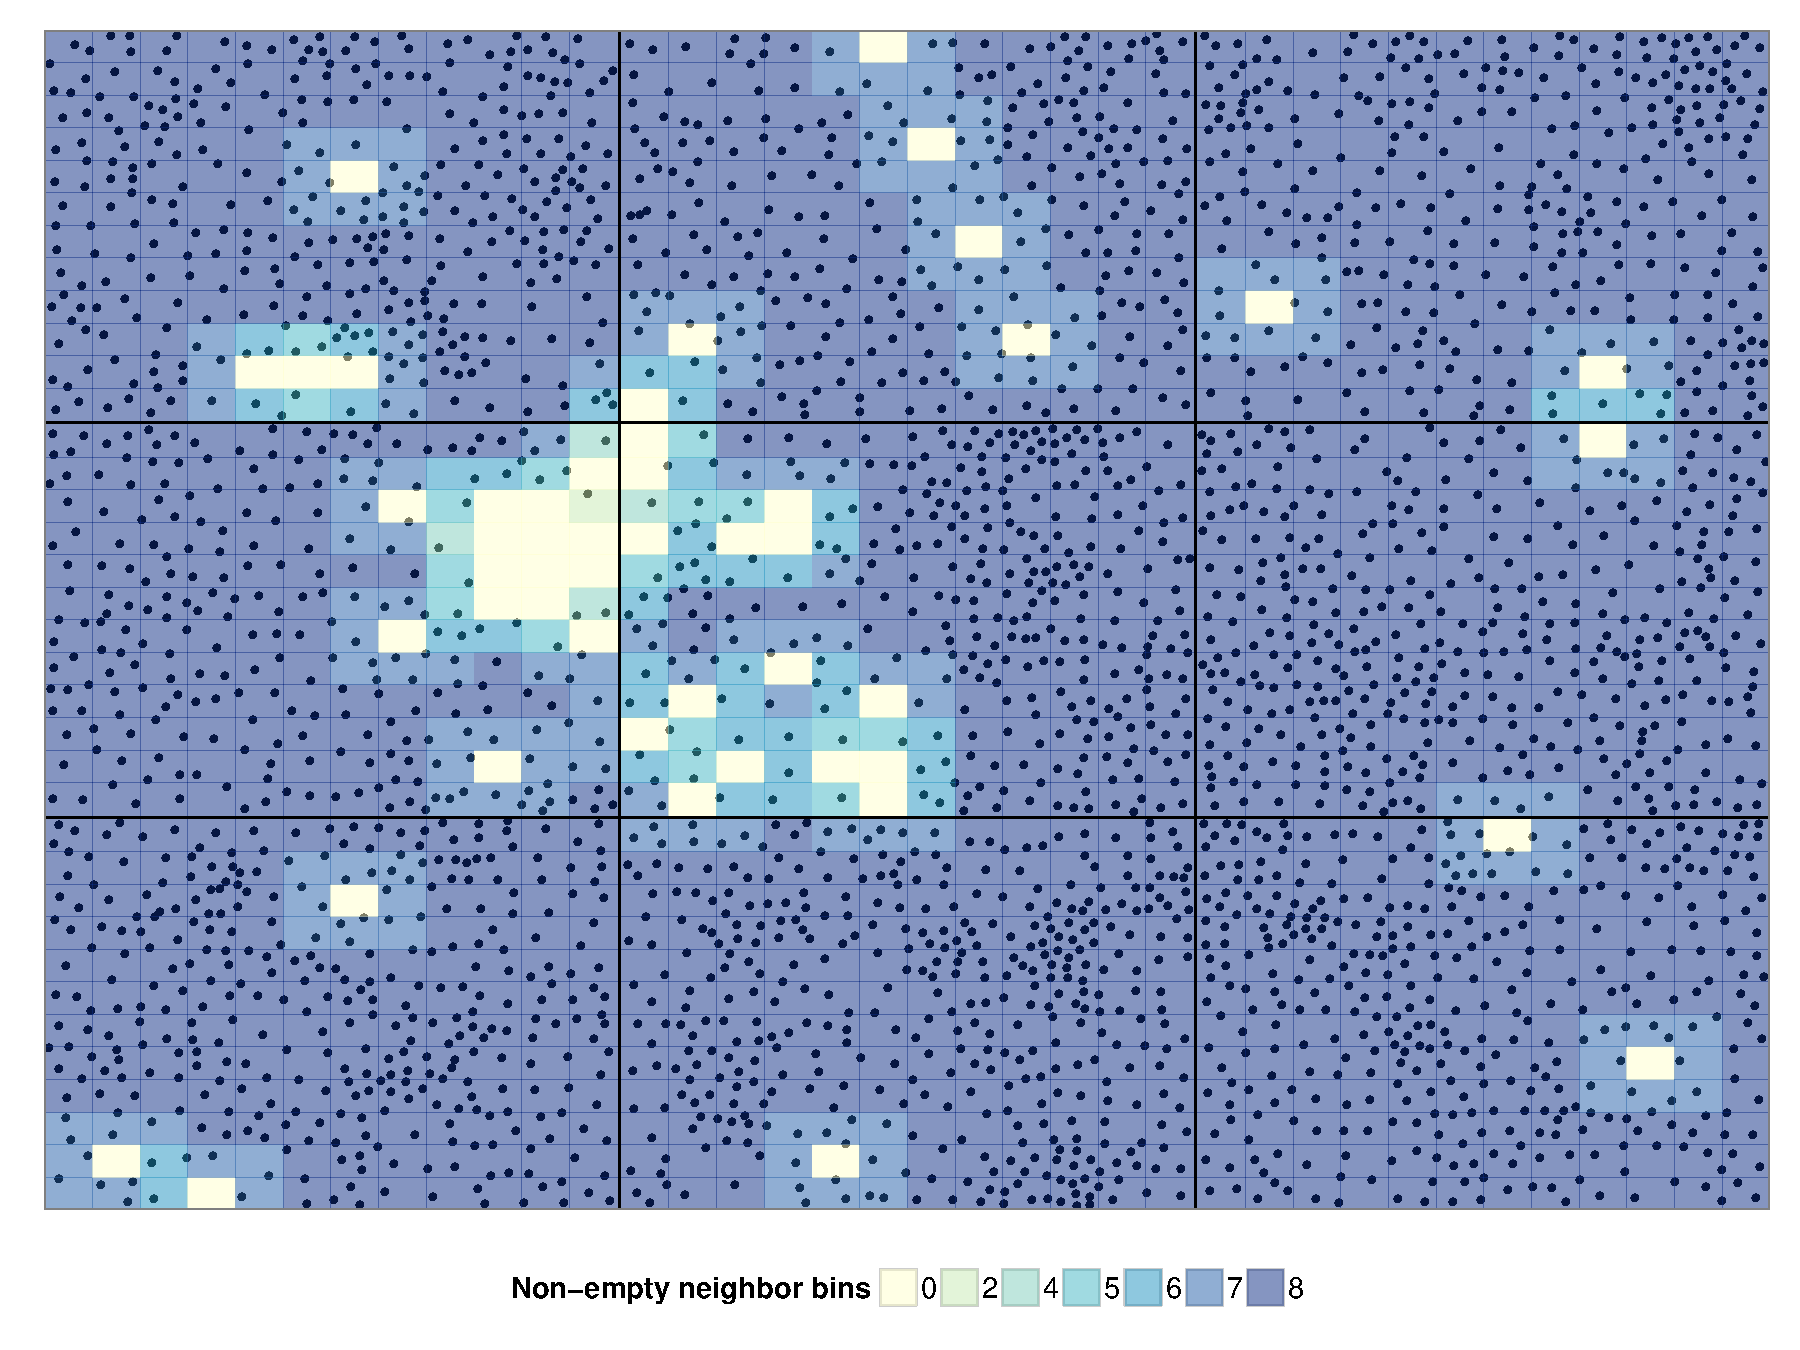
\includegraphics[width=\maxwidth]{figures/R/scf-intro/plot-scf-intro_plot-1} \caption[Visualization of cell colony edge detection by 2D binning.]{Cell colony edges are detected by 2D binning of cell center locations. Dots represent cell centers within the well H6 of plate J107-2C. Each of the nine images is segmented into 12 horizontal and 12 vertical sections yielding 144 tiles (1296 bins for the entire well). The tiles are colored according to the number of non-empty neighboring bins.}\label{fig:scf-intro_plot}
\end{figure}


\end{knitrout}



\newcommand{\knitrScfBenchmarkFacetMean}{\SI{7.77}{\milli\second}}
\newcommand{\knitrScfBenchmarkFacetSd}{\SI{2.69}{\milli\second}}
\newcommand{\knitrScfBenchmarkFacetTotal}{\SI{2.98} s}
\newcommand{\knitrScfBenchmarkEdgeMean}{\SI{515.85}{\milli\second}}
\newcommand{\knitrScfBenchmarkEdgeSd}{\SI{14.66}{\milli\second}}
\newcommand{\knitrScfBenchmarkEdgeTotal}{\SI{198.08}{\second}}
\newcommand{\knitrScfBenchmarkSpeedup}{66}


Times for my version are mean \knitrScfBenchmarkFacetMean\ (with sd \knitrScfBenchmarkFacetSd) and total runtime for a plate is \knitrScfBenchmarkFacetTotal, while theirs runs with mean \knitrScfBenchmarkEdgeMean\ (sd \knitrScfBenchmarkEdgeSd) and for a plate \knitrScfBenchmarkEdgeTotal.
\chapter{InfectX Protocols}

\section{Materials and Methods for Wet-Lab Procedures}
\label{sec:pathogen-protocols}
The following sections describe materials and methods employed in pathogen specific protocols. This information has been published in \cite{Ramo2014} and is only reproduced for the reader's convenience.

\paragraph{\textit{B. henselae}-specific protocol.}
\textit{Bartonella henselae} ATCC49882\textsuperscript{T} \textDelta\textit{bep}G containing plasmid pCD353 \citep{Dehio1998} for IPTG-inducible expression of GFP were grown on Columbia base agar (CBA) plates supplemented with 5\% defibrinated sheep blood (Oxoid) and \SI{50}{\micro\gram\per\milli\litre} kanamycin. Bacteria were incubated at \SI{35}{\celsius} in 5\% \ce{CO2} for \SI{72}{\hour} before re-streaking them on fresh CBA and further growth for \SI{48}{\hour}. Cells were washed once after siRNA-transfection with M199 (Invitrogen)\slash 10\% \gls{fbs} using a plate washer (ELx50-16, BioTek). Cells were infected with \textit{B. henselae} at an \gls{moi} of 400 in \SI{50}{\micro\litre} of M199\slash 10\% \gls{fbs} and \SI{0.5}{\milli\Molar} IPTG (Applichem) and were incubated at \SI{35}{\celsius} in 5\% \ce{CO2} for \SI{30}{\hour}. Fixation at RT was performed using a Multidrop 384 (Thermo Scientific) to wash cells with \SI{50}{\micro\litre} of PBS, fixed in \SI{20}{\micro\litre} of 3.7\% PFA for \SI{10}{\minute}, and washed once more with \SI{50}{\micro\litre} of PBS. Staining was performed on a Biomek liquid handling platform. Fixed cells were washed twice with \SI{25}{\micro\litre} of PBS and blocked in PBS\slash 0.2\% BSA for \SI{10}{\minute}. Extracellular bacteria were labeled with a rabbit serum 2037 against B. henselae \citep{Dehio1997} and a secondary antibody goat anti rabbit A647 (Jackson Immuno) in PBS\slash 0.2\% BSA. Antibodies were incubated for \SI{30}{\minute} each and both incubations were followed by two washings with \SI{25}{\micro\litre} of PBS. Cells were then permeabilized with \SI{20}{\micro\litre} of 0.1\% Triton X-100 (Sigma) for \SI{10}{\minute} and afterwards washed twice with \SI{25}{\micro\litre} of PBS, followed by the addition of \SI{20}{\micro\litre} of staining solution (PBS containing \SI{1.5}{\micro\gram\per\milli\litre} DY-547-Phalloidin, Dyomics and \SI{1}{\micro\gram\per\milli\litre} DAPI, Roche). After \SI{30}{\minute} of incubation in the staining solution, cells were washed twice with \SI{25}{\micro\litre} PBS, followed by a final addition of \SI{50}{\micro\litre} of PBS.

\paragraph{\textit{B. abortus}-specific protocol.}
\textit{Brucella abortus} 2308 pJC43 (\textit{aphT::GFP}) \citep{Celli2005} were grown in tryptic soy broth (TSB) medium containing \SI{50}{\micro\gram\per\milli\litre} kanamycin for \SI{20}{\hour} at \SI{37}{\celsius} and shaking (\SI{100}{\rpm}) to an OD of 0.8--1.1. \SI{50}{\micro\litre} of DMEM\slash 10\% containing bacteria was added per well to obtain a final \gls{moi} of 10000 using a cell plate washer (ELx50-16, BioTek). Plates were then centrifuged at \SI{400}{\gravity} for \SI{20}{\minute} at \SI{4}{\celsius} to synchronize bacterial entry. After \SI{4}{\hour} incubation at \SI{37}{\celsius} and 5\% \ce{CO2}, extracellular bacteria were killed by exchanging the infection medium by \SI{50}{\micro\litre} medium supplemented with 10\% \gls{fbs} and \SI{100}{\micro\gram\per\milli\litre} gentamicin (Sigma). After a total infection time of \SI{44}{\hour} cells were fixed with 3.7\% PFA for \SI{20}{\minute} at RT with the cell plate washer. Staining was performed using a Biomek liquid handling platform. Cells were washed twice with PBS and permeabilized with 0.1\% Triton X (Sigma) for \SI{10}{minute}. Then, cells were washed twice with PBS, followed by addition of \SI{20}{\micro\litre} of staining solution which includes DAPI (\SI{1}{\micro\gram\per\milli\litre}, Roche) and DY-547-phalloidin (\SI{1.5}{\micro\gram\per\milli\litre}, Dyomics) in 0.5\% BSA in PBS. Cells were incubated with staining solution for \SI{30}{\minute} at RT, washed twice with PBS, followed by final addition of \SI{50}{\micro\litre} PBS.

\paragraph{\textit{L. monocytogenes}-specific protocol.}
After washing an overnight culture of \textit{L. monocytogenes} EGDe.PrfA*GFP three times with PBS, bacteria were diluted in DMEM supplemented with 1\% \gls{fbs}. Cells were infected at a \gls{moi} of 25 in \SI{30}{\micro\litre} infection medium per well. After centrifugation at \SI{1000}{\rpm} for \SI{5}{\minute} and incubation for \SI{1}{\hour} at \SI{37}{\celsius} in 5\% \ce{CO2} to allow the bacteria to enter, extracellular bacteria were killed by exchanging the infection medium by \SI{30}{\micro\litre} DMEM supplemented with 10\% \gls{fbs} and \SI{40}{\micro\gram\per\milli\litre} gentamicin (Gibco). Both medium exchange steps were carried out with a plate washer (ELx50-16, BioTek). After additional \SI{4}{\hour} at \SI{37}{\celsius} in a 5\% \ce{CO2} atmosphere, cells were fixed for \SI{15}{\minute} at RT by adding \SI{30}{\micro\litre} of 8\% PFA in PBS to each well using a multidrop 384 device (Thermo Electron Corporation). PFA was removed by four washes with \SI{500}{\micro\litre} PBS per well using the Power Washer 384 (Tecan). Fixed cells were stained for nuclei, actin and bacterially secreted InlC. First, cells were incubated for \SI{30}{\minute} with \SI{10}{\micro\litre} per well of primary staining solution (0.2\% saponin, PBS) containing rabbit derived anti-InlC serum (1:250). After four washes with \SI{40}{\micro\litre} PBS per well cells were stained with \SI{10}{\micro\litre} per well of the secondary staining solution (0.2\% saponin, PBS) containing Alexa Fluor-546 coupled anti-rabbit antibody (1:250, Invitrogen), DAPI (\SI{0.7}{\micro\gram\per\milli\litre}, Roche), and DY-647-Phalloidin (\SI{2}{\micro\gram\per\milli\litre}, Dyomics). After four washes with \SI{40}{\micro\litre} PBS per well, the cells were kept in \SI{40}{\micro\litre} PBS per well. The staining procedure was carried out with a Tecan freedom evo robot.

\paragraph{\textit{S.} typhimurium-specific protocol.}
All liquid handing stages of infection, fixation, and immunofluorescence staining were performed on a liquid handling robot (BioTek; EL406). For infection the \textit{S.} typhimurium strain S.Tm\textsuperscript{SopE\_pM975} was used. This strain is a single effector strain, only expressing SopE out of the main four SPI-1 encoded effectors (SipA, SopB, SopE2 and SopE). Additionally this strain harbors a plasmid (pM975) that expresses GFP under the control of a SPI2 (ssaG)-dependent promotor. The bacterial solution was prepared by cultivating a \SI{12}{\hour} culture in \SI{0.3}{\Molar} LB medium containing \SI{50}{\micro\gram\per\milli\litre} streptomycin and \SI{50}{\micro\gram\per\milli\litre} ampicillin. Afterwards a \SI{4}{\hour} subculture (1:20 diluted from the \SI{12}{\hour} culture) was cultivated in \SI{0.3}{\Molar} LB medium containing \SI{50}{\micro\gram\per\milli\litre} streptomycin, which reached an OD\textunderscript{600nm}$\approx1.0$ after the respective \SI{4}{\hour} of incubation time. To perform the infection, \SI{16}{\micro\litre} of diluted \textit{S.} typhimurium (\gls{moi} of 80) were added to the HeLa cells. After \SI{20}{\minute} of incubation at \SI{37}{\celsius} and 5\% \ce{CO2}, the \textit{S.} typhimurium-containing media was replaced by \SI{60}{\micro\litre} DMEM\slash 10\% \gls{fbs} containing \SI{50}{\micro\gram\per\micro\litre} streptomycin and \SI{400}{\micro\gram\per\micro\litre} gentamicin to kill all remaining extracellular bacteria. After additional \SI{3}{\hour} \SI{40}{\minute} incubation at \SI{37}{\celsius} and 5\% \ce{CO2}, cells were fixed by adding \SI{35}{\micro\litre} 4\% PFA, 4\% sucrose in PBS for \SI{20}{\minute} at RT. The fixation solution was removed by adding \SI{60}{\micro\litre} PBS containing \SI{400}{\micro\gram\per\milli\litre} gentamicin. Cells were permeabilized for \SI{5}{\minute} with \SI{40}{\micro\litre} 0.1\% Triton X-100 (Sigma-Aldrich). Afterwards \SI{24}{\micro\litre} of staining solution containing DAPI (1:1000, Sigma-Aldrich) and DY-547-phalloidin (\SI{1.2}{\micro\gram\per\milli\litre}, Dyomics) was added (prepared in blocking buffer consisting of 4\% BSA and 4\% Sucrose in PBS). After \SI{1}{\hour} of incubation at RT, cells were washed three times with PBS followed by the addition of \SI{60}{\micro\litre} PBS containing \SI{400}{\micro\gram\per\milli\litre} gentamicin.

\paragraph{\textit{S. flexneri}-specific protocol.}
\textit{S. flexneri} M90T \textDelta\textit{vir}G pCK100 (PuhpT::dsRed) were harvested in exponential growth phase and coated with 0.005\% poly-L-lysine (Sigma-Aldrich). Afterwards, bacteria were washed with PBS and resuspended in assay medium (DMEM, \SI{2}{\milli\Molar} L-Glutamine, \SI{10}{\milli\Molar} HEPES). \SI{20}{\micro\litre} of bacterial suspension was added to each well with a final \gls{moi} of 15. Plates were then centrifuged for \SI{1}{\minute} at \SI{37}{\celsius} and incubated at \SI{37}{\celsius} and 5\% \ce{CO2}. After \SI{30}{\minute} of infection, \SI{75}{\micro\litre} were aspirated from each well and monensin (Sigma) and gentamicin (Gibco) were added to a final concentration of \SI{66.7}{\micro\Molar} and \SI{66.7}{\micro\gram\per\milli\litre}, respectively. After a total infection time of \SI{3.5}{\hour}, cells were fixed in 4\% PFA for \SI{10}{\minute}. Liquid handling was performed using the Multidrop 384 (Thermo Scientific) for dispension steps and a plate washer (ELx50-16, BioTek) for aspiration steps. For immunofluorescent staining, cells were washed with PBS using the Power Washer 384 (Tecan). Subsequently, cells were incubated with a mouse anti-human \gls{il-8} antibody (1:300, BD Biosciences) in staining solution (0.2\% saponin in PBS) for \SI{2}{\hour} at RT. After washing the cells with PBS, Hoechst (\SI{5}{\micro\gram\per\milli\litre}, Invitrogen), DY-495-phalloidin (\SI{1.2}{\micro\gram\per\milli\litre}, Dyomics) and Alexa Fluor 647-coupled goat anti-mouse IgG (1:400, Invitrogen) were added and incubated for \SI{1}{\hour} at RT. The staining procedure was performed using the Biomek NXP Laboratory Automation Workstation (Beckman Coulter).

\paragraph{Adenovirus-specific protocol.}
All liquid handling stages of infection, fixation, and immunofluorescence staining were performed on the automated pipetting system Well Mate (Thermo Scientific Matrix) and washer Hydrospeed (Tecan). For infection screens recombinant Ad2\_\textDelta E3B-eGFP (short Adenovirus) was utilized as described before \citep{Suomalainen2013,Yakimovich2012}. Adenovirus was added to cells at an \gls{moi} of 0.1 in \SI{10}{\micro\litre} of an infection media\slash FBS (DMEM supplemented with L-glutamine, 10\% FBS, 1\% Pen\slash Strep, Invitrogen). Screening plates were incubated at \SI{37}{\celsius} for \SI{16}{\hour}, and cells were fixed by adding \SI{21}{\micro\litre} of 16\% PFA directly to the cells in culture media for \SI{45}{\minute} at RT or long-term storage at \SI{4}{\celsius}. Cells were washed 2 times with PBS\slash \SI{25}{\milli\Molar} \ce{NH4Cl}, permeabilized with \SI{25}{\micro\litre} 0.1\% Triton X-100 (Pharmaciebiothek). After 2 washes with PBS the samples were incubated at RT for \SI{1}{\hour} with \SI{25}{\micro\litre} staining solution (PBS) containing DAPI (\SI{1}{\micro\gram\per\milli\litre}, Sigma-Aldrich) and DY-647-phalloidin (\SI{1}{\micro\gram\per\milli\litre}, Dyomics), washed 2 times with PBS and stored until imaging in \SI{50}{\micro\litre} PBS\slash \ce{NaN3}.

\paragraph{Rhinovirus-specific protocol.}
All liquid handling stages of infection, fixation, and immunofluorescence staining were performed on the automated pipetting system Well Mate (Thermo Scientific Matrix) and washer Hydrospeed (Tecan). For infection assays with human Rhinovirus serotype 1a (HRV1a) were carried out as described, except that the anti-VP2 antibody Mab 16\slash 7 was used for staining of the infected cells as described earlier \citep{Jurgeit2012,Jurgeit2010,Mosser2002}. Rhinovirus at an \gls{moi} of 8 was added to cells in \SI{20}{\micro\litre} of an infection media\slash BSA (DMEM supplemented with GlutaMAX, \SI{30}{\milli\Molar} \ce{MgCl2} and 0.2\% BSA, Invitrogen). Screening plates were incubated for \SI{7}{\hour} at \SI{37}{\celsius}, and cells were fixed by adding \SI{33}{\micro\litre} of 16\% PFA directly to the culture medium. Fixation was either for \SI{30}{\minute} at RT or long term storage at \SI{4}{\celsius}. Cells were washed twice with PBS\slash \SI{25}{\milli\Molar} \ce{H2O}, permeabilized with \SI{50}{\micro\litre} 0.2\% Triton X-100 (Sigma- Aldrich) followed by 3 PBS washes and blocking with PBS containing 1\% BSA (Fraction V, Sigma-Aldrich). Fixed and permeabilized cells were incubated at RT for \SI{1}{\hour} with diluted mabR16-7 antibody (\SI{0.45}{\micro\gram\per\milli\litre}) in PBS\slash 1\% BSA. Cells were washed 3 times with PBS and incubated with \SI{25}{\micro\litre} secondary staining solution (PBS\slash 1\% BSA) containing Alexa Fluor 488 secondary antibody (\SI{1}{\micro\gram\per\milli\litre}, Invitrogen), DAPI (\SI{1}{\micro\gram\per\milli\litre}, Sigma-Aldrich), and DY-647-phalloidin (\SI{0.2}{\micro\gram\per\milli\litre}, Dyomics). Cells were washed twice with PBS after \SI{2}{\hour} of incubation in secondary staining solution and stored in \SI{50}{\micro\litre} PBS\slash \ce{NaN3}.

\paragraph{Vacciniavirus-specific protocol.}
All liquid handing stages of infection, fixation, and immunofluorescence staining were performed on a liquid handling robot (BioTek, EL406). For infection assays a recombinant WR VACV, WR E EGFP\slash L mCherry, was utilized. For infection, media was aspirated from the RNAi-transfected cell plates and replaced with \SI{40}{\micro\litre} of virus solution per well (\gls{moi} of 0.125). Screening plates were incubated for \SI{1}{\hour} at \SI{37}{\celsius} to allow for infection, after which virus-containing media was removed and replaced with \SI{40}{\micro\litre} DMEM\slash 10\% \gls{fbs}. \SI{8}{\hour} after infection \SI{40}{\micro\litre} of DMEM\slash 10\% \gls{fbs} containing \SI{20}{\micro\Molar} cytosine arabinoside (AraC) was added to all wells to prevent virus DNA replication in secondary infected cells. \SI{24}{\hour} after infection cells were fixed by the addition of \SI{20}{\micro\litre} 18\% PFA for \SI{30}{\minute} followed by two PBS washes of \SI{80}{\micro\litre}. For immunofluorescence staining of EGFP, cells were incubated for \SI{2}{\hour} in \SI{30}{\micro\litre} primary staining solution (0.5\% Triton X-100, 0.5\% BSA, PBS) per well, containing anti-GFP antibody (1:1000). Cells were washed twice in \SI{80}{\micro\litre} PBS, followed by the addition of \SI{30}{\micro\litre} secondary staining solution (0.5\% BSA, PBS) containing Alexa Fluor 488 secondary antibody (1:1000), Hoechst (1:10000), and DY-647-phalloidin (1:1200, Dyomics). Cells were washed twice with \SI{80}{\micro\litre} PBS after \SI{1}{\hour} incubation in secondary staining solution followed by the addition of \SI{80}{\micro\litre} \ce{H2O}.

\section{Decision Trees for Infection Scoring}
The decision trees for adenovirus and \textit{Bartonella} are shown in section~\ref{sec:infection-scoring} while the ones corresponding to the remaining pathogens (\textit{Brucella}, \textit{Listeria}, rhinovirus, \textit{Salmonella} and vaccinia virus) follow. Please refer to section~\ref{sec:infection-scoring} for more information of infection scoring.

\begin{figure}[b]
\centering
\begin{tikzpicture}

\node [decision={$> 0.050$}{$\le 0.050$}] { 
  \texttt{Nuclei.Intensity\_MeanIntensity\_\\CorrPathogen}
}
[decision tree]
child { node [outcome] { infected } }
child { node [decision={$> 0.055$}{$\le 0.055$}] { 
\texttt{PeriNuclei.Intensity\_MeanIntensity\_\\CorrPathogen} } 
  child { node [outcome] { infected } }
  child { node [decision={$> 0.075$}{$\le 0.075$}] { 
  \texttt{Cells.Intensity\_MeanIntensity\_\\CorrPathogen} }
    child { node [outcome] { infected } }
    child { node [outcome] { not infected } }
  }
};

\end{tikzpicture}
\caption[Decision tree for \textit{Brucella} infection scoring.]{Decision tree for \textit{Brucella} infection scoring. While the first two decisions are modeled to capture what is considered a normal infection pattern, the last split imposes a high threshold for cells that have failed the first two steps to still be considered infected.}
\end{figure}

\begin{figure}
\centering
\begin{tikzpicture}

\node [decision={$> 0.11$}{$\le 0.11$}] { 
  \texttt{Nuclei.Intensity\_MeanIntensity\_\\CorrInlC}
}
[decision tree]
child { node [outcome] { infected } }
child { node [decision={$> 0.15$}{$\le 0.15$}] { 
\texttt{PeriNuclei.Intensity\_MeanIntensity\_\\CorrInlC} } 
  child { node [outcome] { infected } }
  child { node [decision={$> 0.12$}{$\le 0.12$}] { 
  \texttt{Nuclei.Intensity\_UpperQuartileIntensity\_\\CorrInlC} }
    child { node [outcome] { infected } }
    child { node [outcome] { not infected } }
  }
};

\end{tikzpicture}
\caption[Decision tree for \textit{Listeria} infection scoring.]{The decision tree for \textit{Listeria} infection scoring is based on a channel recording InlC localization and intensity instead of targeting the bacteria themselves.}
\end{figure}

\begin{figure}
\centering
\begin{tikzpicture}

\node [decision={$> 0.085$}{$\le 0.085$}] { 
  \texttt{Nuclei.Intensity\_MeanUpperTenPercent-\\Intensity\_CorrPathogen}
}
[decision tree]
child { node [outcome] { infected } }
child { node [decision={$> 0.090$}{$\le 0.090$}] { 
\texttt{PeriNuclei.Intensity\_MeanUpperTen-\\PercentIntensity\_CorrPathogen} } 
  child { node [outcome] { infected } }
  child { node [decision={$> 0.125$}{$\le 0.125$}] { 
  \texttt{VoronoiCells.Intensity\_MeanUpperTen-\\PercentIntensity\_CorrPathogen} }
    child { node [outcome] { infected } }
    child { node [outcome] { not infected } }
  }
};

\end{tikzpicture}
\caption[Decision tree for rhinovirus infection scoring.]{Decision tree for rhinovirus infection scoring. Using the mean of the uppermost decile of pathogen channel intensity data yields the most table results.}
\end{figure}

\begin{figure}
\centering
\begin{tikzpicture}

\node [decision={$> 0.085$}{$\le 0.085$}] { 
  \texttt{Cells.Intensity\_SubCell-\\BacteriaMeanIntensity\_CorrPathogen}
}
[decision tree]
child { node [decision={$< 2$}{$\ge 2$}] { 
  \texttt{Cells.AreaShape\_SubCellBacteria-\\Area\_CorrPathogen} }
  child { node [outcome] { infected } }
  child { node [outcome] { not infected } }
}
child { node [outcome] { not infected } };

\end{tikzpicture}
\caption[Decision tree for \textit{Salmonella} infection scoring.]{Decision tree for \textit{Salmonella} infection scoring. For a cell being considered infected, not only does the threshold for pathogen intensity throughout the cell need be exceeded but the bacteria also have to be sufficiently aggregated.}
\end{figure}

\begin{figure}
\centering
\begin{tikzpicture}

\node [decision={$> 0.045$}{$\le 0.045$}] { 
  \texttt{Nuclei.Intensity\_MeanIntensity\_\\Corr1Pathogen}
}
[decision tree]
child { node [outcome] { infected } }
child { node [decision={$> 0.050$}{$\le 0.050$}] { 
\texttt{PeriNuclei.Intensity\_MeanIntensity\_\\Corr1Pathogen} } 
  child { node [outcome] { infected } }
  child { node [outcome] { not infected } }
};

\end{tikzpicture}
\caption[Decision tree for vaccinia virus infection scoring.]{Decision tree for vaccinia virus infection scoring. A separate decision tree for distinguishing primary from secondary infections has been developed but is not shown.}
\end{figure}


\backmatter

%%%%%%%%%%%%%%%%%%%%%%%%%%%%%%%%%%%%%%%%%%%%%%%%%%%%%%%%%%%%%%%%%%%%%%%%%%%%%%%
%%%  Bibliography                                                           %%%
%%%%%%%%%%%%%%%%%%%%%%%%%%%%%%%%%%%%%%%%%%%%%%%%%%%%%%%%%%%%%%%%%%%%%%%%%%%%%%%

\bibliographystyle{chicago}
\bibliography{mendeley}

\addcontentsline{toc}{chapter}{Epilogue}
\chapter*{Epilogue}
\label{s:Epilogue}

A few final words. Test 2

\begin{knitrout}
\definecolor{shadecolor}{rgb}{0.969, 0.969, 0.969}\color{fgcolor}\begin{figure}

{\centering 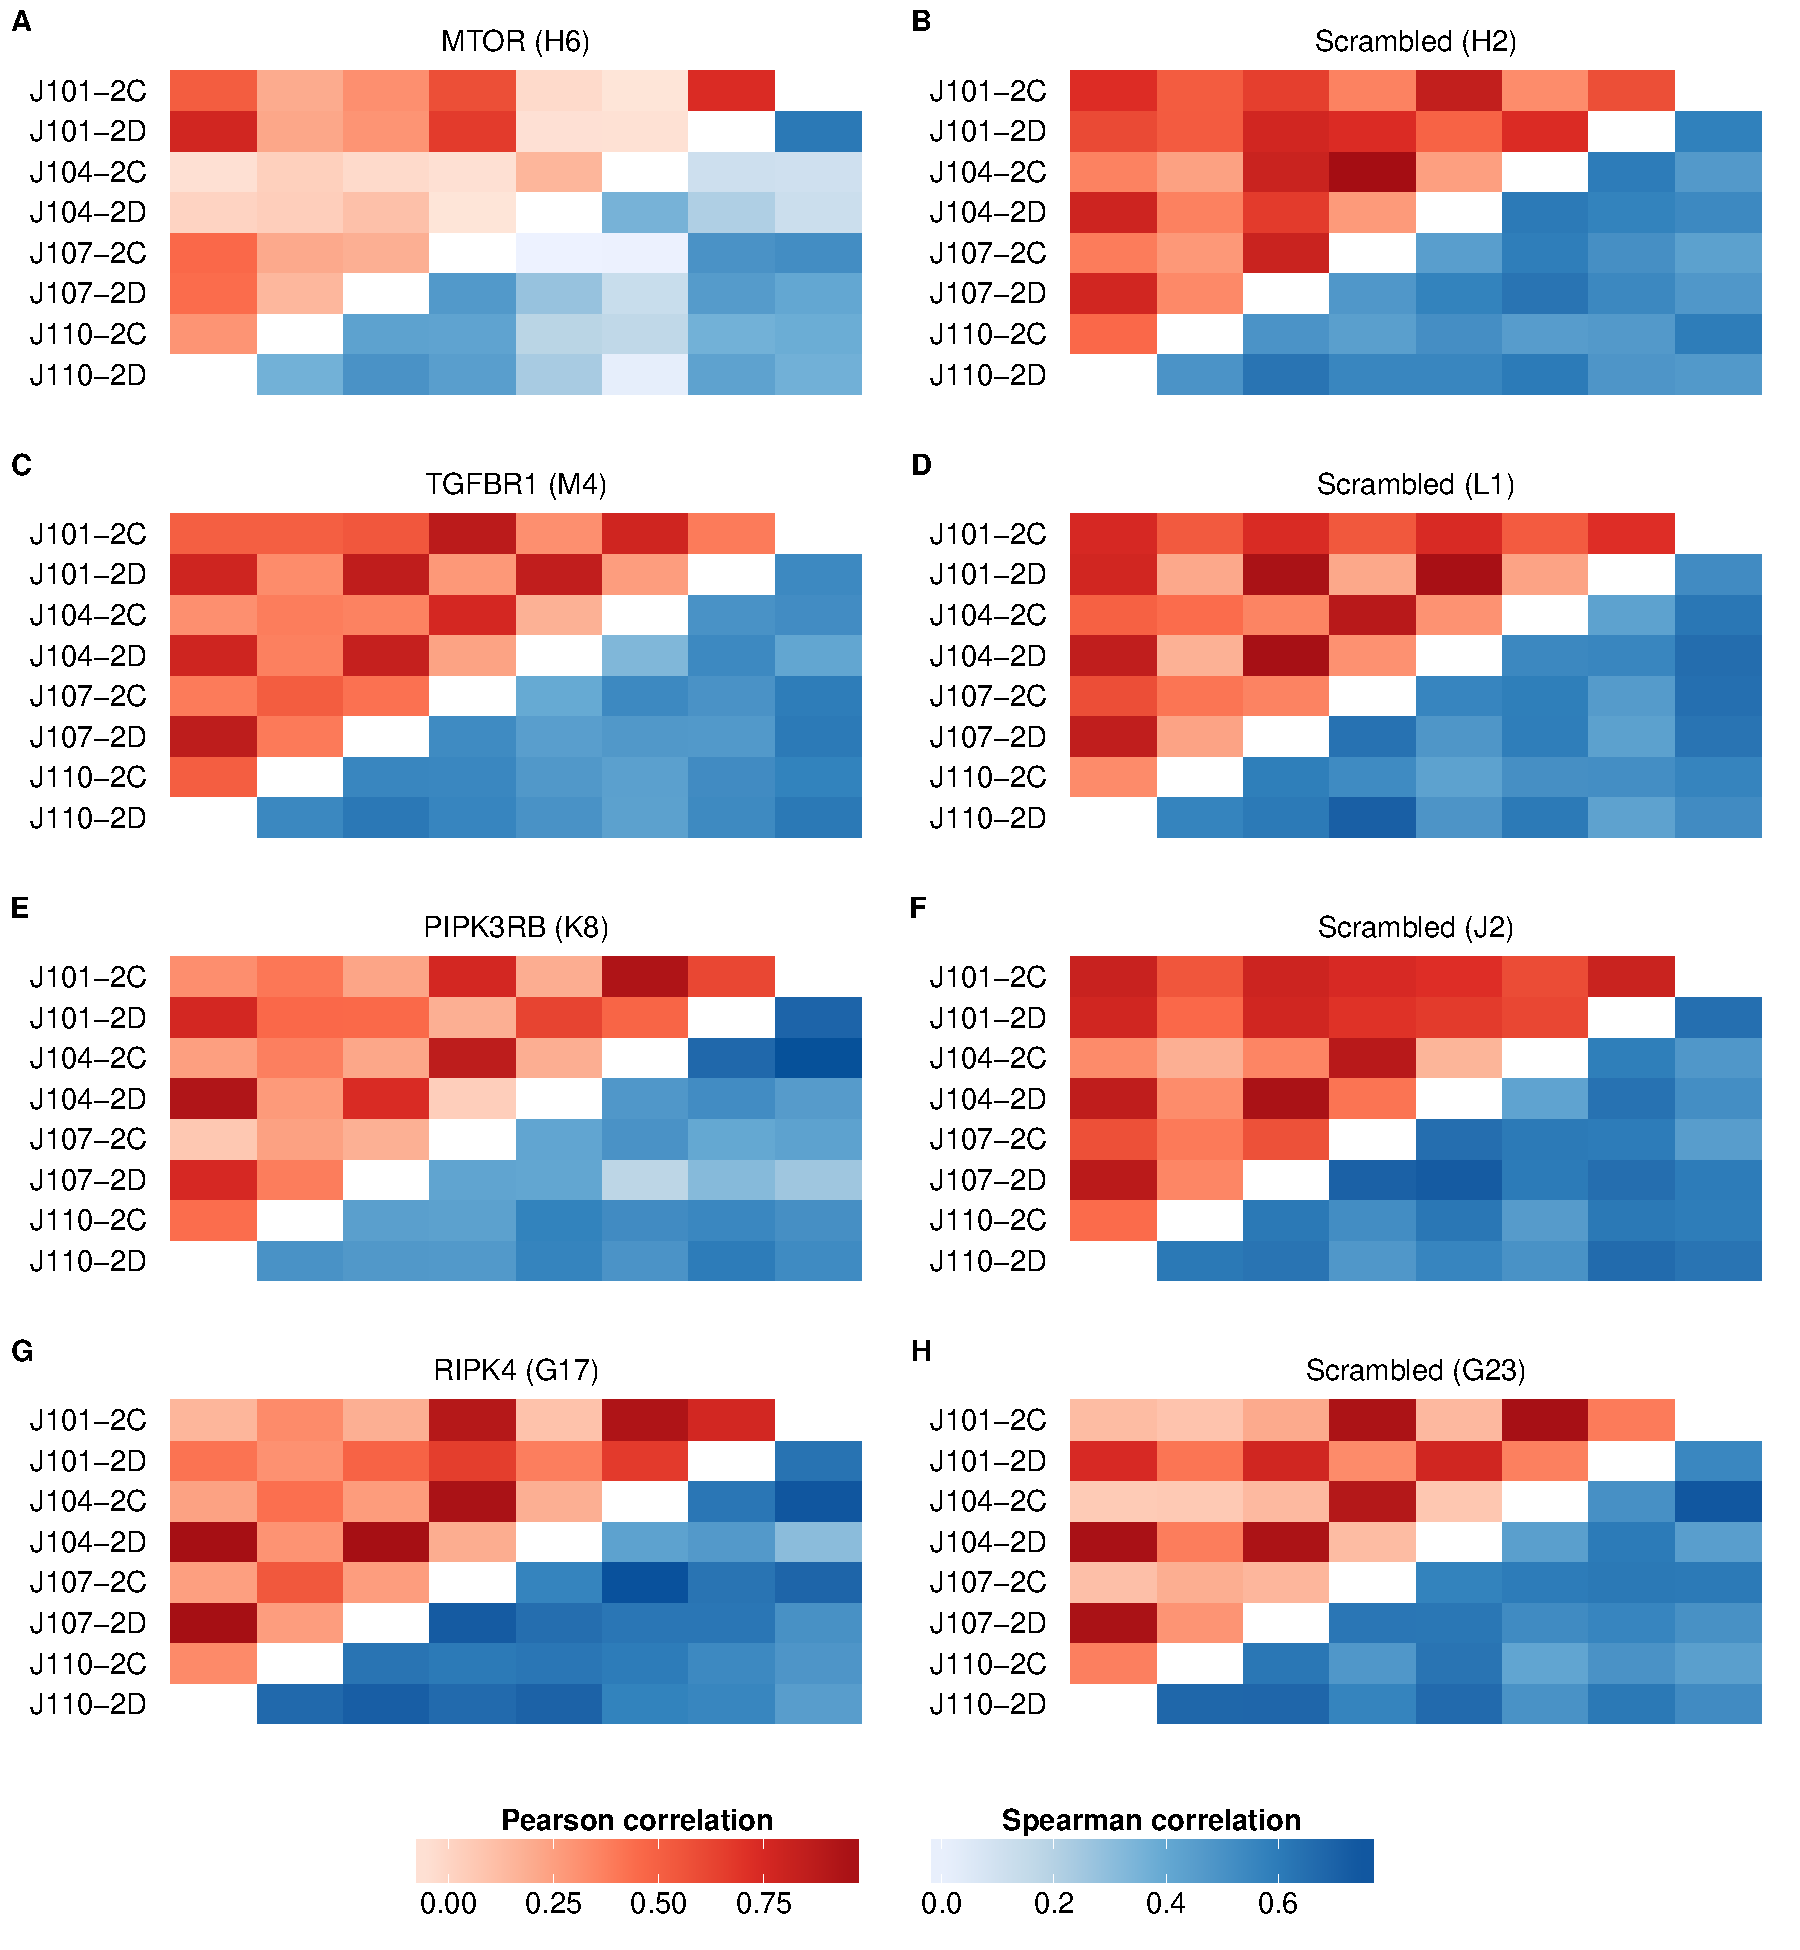
\includegraphics[width=\maxwidth]{figures/R/forest-corr-forest-corr-1} 

}

\caption[Heatmap representations of Pearson and Spearman correlation among feature importance scores obtained by random forest analysis.]{Heatmap representations of correlation matrices obtained by comparing importance scores of features as determined by random forest analysis. Red shades indicate Pearson correlation while blue shades visualize Spearman's rank correlation coefficients. For each gene and scrambled well, all available 8 replicates of the \textit{Brucella} Dharmacon unpooled dataset were considered.}\label{fig:forest-corr}
\end{figure}


\end{knitrout}



%%% Local Variables: 
%%% mode: latex
%%% TeX-master: "00_Master"
%%% End: 


%%%%%%%%%%%%%%%%%%%%%%%%%%%%%%%%%%%%%%%%%%%%%%%%%%%%%%%%%%%%%%%%%%%%%%%%%%%%%%%
%%%  Declaration of originality                                             %%%
%%%%%%%%%%%%%%%%%%%%%%%%%%%%%%%%%%%%%%%%%%%%%%%%%%%%%%%%%%%%%%%%%%%%%%%%%%%%%%%

\cleartorecto
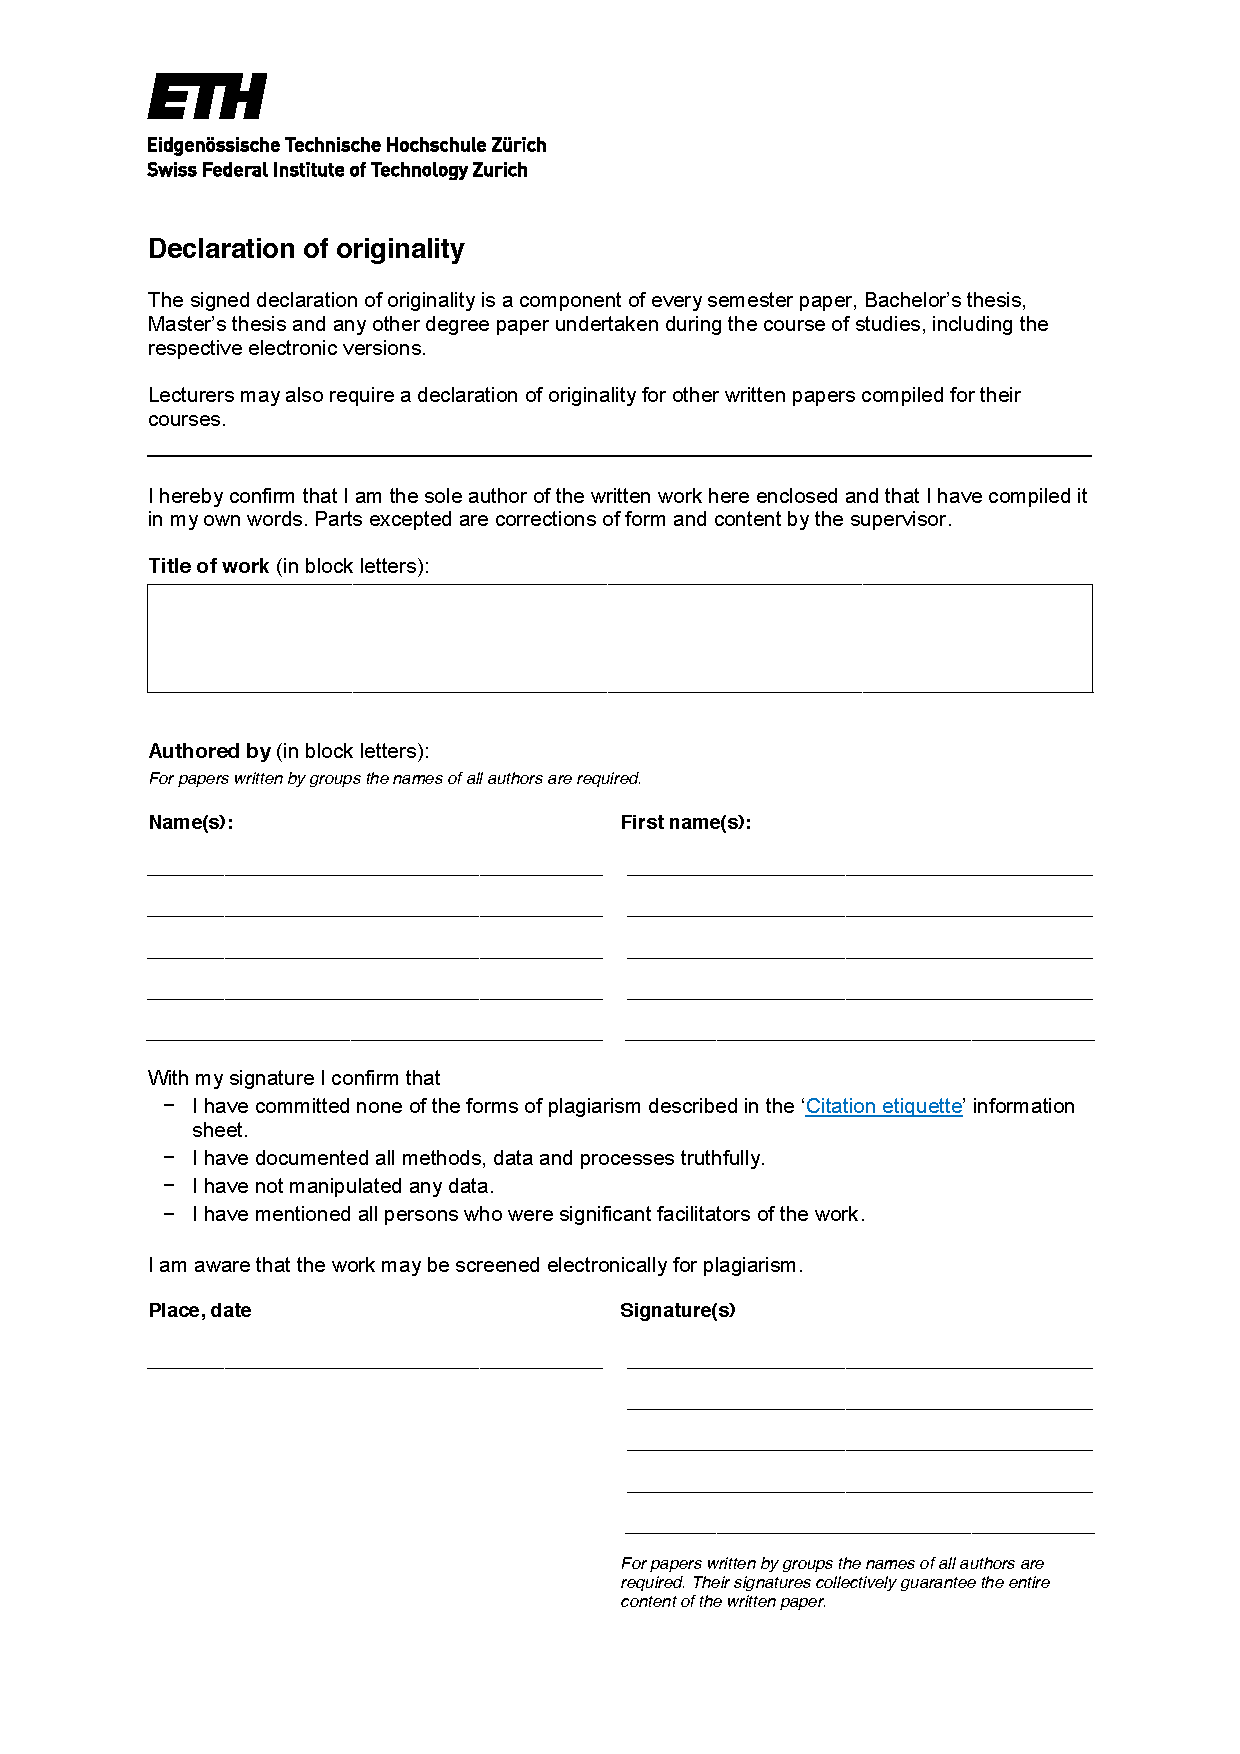
\includepdf[pages={-}]{declaration-originality.pdf}

\end{document}
